\documentclass[]{book}
\usepackage{lmodern}
\usepackage{amssymb,amsmath}
\usepackage{ifxetex,ifluatex}
\usepackage{fixltx2e} % provides \textsubscript
\ifnum 0\ifxetex 1\fi\ifluatex 1\fi=0 % if pdftex
  \usepackage[T1]{fontenc}
  \usepackage[utf8]{inputenc}
\else % if luatex or xelatex
  \ifxetex
    \usepackage{mathspec}
  \else
    \usepackage{fontspec}
  \fi
  \defaultfontfeatures{Ligatures=TeX,Scale=MatchLowercase}
\fi
% use upquote if available, for straight quotes in verbatim environments
\IfFileExists{upquote.sty}{\usepackage{upquote}}{}
% use microtype if available
\IfFileExists{microtype.sty}{%
\usepackage{microtype}
\UseMicrotypeSet[protrusion]{basicmath} % disable protrusion for tt fonts
}{}
\usepackage[margin=1in]{geometry}
\usepackage{hyperref}
\hypersetup{unicode=true,
            pdftitle={Linear Regression 101},
            pdfauthor={Alfonso R. Reyes},
            pdfborder={0 0 0},
            breaklinks=true}
\urlstyle{same}  % don't use monospace font for urls
\usepackage{natbib}
\bibliographystyle{apalike}
\usepackage{color}
\usepackage{fancyvrb}
\newcommand{\VerbBar}{|}
\newcommand{\VERB}{\Verb[commandchars=\\\{\}]}
\DefineVerbatimEnvironment{Highlighting}{Verbatim}{commandchars=\\\{\}}
% Add ',fontsize=\small' for more characters per line
\usepackage{framed}
\definecolor{shadecolor}{RGB}{248,248,248}
\newenvironment{Shaded}{\begin{snugshade}}{\end{snugshade}}
\newcommand{\AlertTok}[1]{\textcolor[rgb]{0.94,0.16,0.16}{#1}}
\newcommand{\AnnotationTok}[1]{\textcolor[rgb]{0.56,0.35,0.01}{\textbf{\textit{#1}}}}
\newcommand{\AttributeTok}[1]{\textcolor[rgb]{0.77,0.63,0.00}{#1}}
\newcommand{\BaseNTok}[1]{\textcolor[rgb]{0.00,0.00,0.81}{#1}}
\newcommand{\BuiltInTok}[1]{#1}
\newcommand{\CharTok}[1]{\textcolor[rgb]{0.31,0.60,0.02}{#1}}
\newcommand{\CommentTok}[1]{\textcolor[rgb]{0.56,0.35,0.01}{\textit{#1}}}
\newcommand{\CommentVarTok}[1]{\textcolor[rgb]{0.56,0.35,0.01}{\textbf{\textit{#1}}}}
\newcommand{\ConstantTok}[1]{\textcolor[rgb]{0.00,0.00,0.00}{#1}}
\newcommand{\ControlFlowTok}[1]{\textcolor[rgb]{0.13,0.29,0.53}{\textbf{#1}}}
\newcommand{\DataTypeTok}[1]{\textcolor[rgb]{0.13,0.29,0.53}{#1}}
\newcommand{\DecValTok}[1]{\textcolor[rgb]{0.00,0.00,0.81}{#1}}
\newcommand{\DocumentationTok}[1]{\textcolor[rgb]{0.56,0.35,0.01}{\textbf{\textit{#1}}}}
\newcommand{\ErrorTok}[1]{\textcolor[rgb]{0.64,0.00,0.00}{\textbf{#1}}}
\newcommand{\ExtensionTok}[1]{#1}
\newcommand{\FloatTok}[1]{\textcolor[rgb]{0.00,0.00,0.81}{#1}}
\newcommand{\FunctionTok}[1]{\textcolor[rgb]{0.00,0.00,0.00}{#1}}
\newcommand{\ImportTok}[1]{#1}
\newcommand{\InformationTok}[1]{\textcolor[rgb]{0.56,0.35,0.01}{\textbf{\textit{#1}}}}
\newcommand{\KeywordTok}[1]{\textcolor[rgb]{0.13,0.29,0.53}{\textbf{#1}}}
\newcommand{\NormalTok}[1]{#1}
\newcommand{\OperatorTok}[1]{\textcolor[rgb]{0.81,0.36,0.00}{\textbf{#1}}}
\newcommand{\OtherTok}[1]{\textcolor[rgb]{0.56,0.35,0.01}{#1}}
\newcommand{\PreprocessorTok}[1]{\textcolor[rgb]{0.56,0.35,0.01}{\textit{#1}}}
\newcommand{\RegionMarkerTok}[1]{#1}
\newcommand{\SpecialCharTok}[1]{\textcolor[rgb]{0.00,0.00,0.00}{#1}}
\newcommand{\SpecialStringTok}[1]{\textcolor[rgb]{0.31,0.60,0.02}{#1}}
\newcommand{\StringTok}[1]{\textcolor[rgb]{0.31,0.60,0.02}{#1}}
\newcommand{\VariableTok}[1]{\textcolor[rgb]{0.00,0.00,0.00}{#1}}
\newcommand{\VerbatimStringTok}[1]{\textcolor[rgb]{0.31,0.60,0.02}{#1}}
\newcommand{\WarningTok}[1]{\textcolor[rgb]{0.56,0.35,0.01}{\textbf{\textit{#1}}}}
\usepackage{longtable,booktabs}
\usepackage{graphicx,grffile}
\makeatletter
\def\maxwidth{\ifdim\Gin@nat@width>\linewidth\linewidth\else\Gin@nat@width\fi}
\def\maxheight{\ifdim\Gin@nat@height>\textheight\textheight\else\Gin@nat@height\fi}
\makeatother
% Scale images if necessary, so that they will not overflow the page
% margins by default, and it is still possible to overwrite the defaults
% using explicit options in \includegraphics[width, height, ...]{}
\setkeys{Gin}{width=\maxwidth,height=\maxheight,keepaspectratio}
\IfFileExists{parskip.sty}{%
\usepackage{parskip}
}{% else
\setlength{\parindent}{0pt}
\setlength{\parskip}{6pt plus 2pt minus 1pt}
}
\setlength{\emergencystretch}{3em}  % prevent overfull lines
\providecommand{\tightlist}{%
  \setlength{\itemsep}{0pt}\setlength{\parskip}{0pt}}
\setcounter{secnumdepth}{5}
% Redefines (sub)paragraphs to behave more like sections
\ifx\paragraph\undefined\else
\let\oldparagraph\paragraph
\renewcommand{\paragraph}[1]{\oldparagraph{#1}\mbox{}}
\fi
\ifx\subparagraph\undefined\else
\let\oldsubparagraph\subparagraph
\renewcommand{\subparagraph}[1]{\oldsubparagraph{#1}\mbox{}}
\fi

%%% Use protect on footnotes to avoid problems with footnotes in titles
\let\rmarkdownfootnote\footnote%
\def\footnote{\protect\rmarkdownfootnote}

%%% Change title format to be more compact
\usepackage{titling}

% Create subtitle command for use in maketitle
\providecommand{\subtitle}[1]{
  \posttitle{
    \begin{center}\large#1\end{center}
    }
}

\setlength{\droptitle}{-2em}

  \title{Linear Regression 101}
    \pretitle{\vspace{\droptitle}\centering\huge}
  \posttitle{\par}
    \author{Alfonso R. Reyes}
    \preauthor{\centering\large\emph}
  \postauthor{\par}
      \predate{\centering\large\emph}
  \postdate{\par}
    \date{2019-09-16}

\usepackage{booktabs}

\begin{document}
\maketitle

{
\setcounter{tocdepth}{1}
\tableofcontents
}
\hypertarget{prerequisites}{%
\chapter*{Prerequisites}\label{prerequisites}}
\addcontentsline{toc}{chapter}{Prerequisites}

This is a \emph{sample} book written in \textbf{Markdown}. You can use anything that Pandoc's Markdown supports, e.g., a math equation \(a^2 + b^2 = c^2\).

The \textbf{bookdown} package can be installed from CRAN or Github:

\begin{Shaded}
\begin{Highlighting}[]
\KeywordTok{install.packages}\NormalTok{(}\StringTok{"bookdown"}\NormalTok{)}
\CommentTok{# or the development version}
\CommentTok{# devtools::install_github("rstudio/bookdown")}
\end{Highlighting}
\end{Shaded}

Remember each Rmd file contains one and only one chapter, and a chapter is defined by the first-level heading \texttt{\#}.

To compile this example to PDF, you need XeLaTeX. You are recommended to install TinyTeX (which includes XeLaTeX): \url{https://yihui.name/tinytex/}.

\hypertarget{temperature-modeling-using-nested-dataframes}{%
\chapter{Temperature modeling using nested dataframes}\label{temperature-modeling-using-nested-dataframes}}

\hypertarget{prepare-the-data}{%
\section{Prepare the data}\label{prepare-the-data}}

\url{http://ijlyttle.github.io/isugg_purrr/presentation.html\#(1)}

\hypertarget{packages-to-run-this-presentation}{%
\subsection{Packages to run this presentation}\label{packages-to-run-this-presentation}}

\begin{Shaded}
\begin{Highlighting}[]
\KeywordTok{library}\NormalTok{(}\StringTok{"readr"}\NormalTok{)}
\KeywordTok{library}\NormalTok{(}\StringTok{"tibble"}\NormalTok{)}
\KeywordTok{library}\NormalTok{(}\StringTok{"dplyr"}\NormalTok{)}
\KeywordTok{library}\NormalTok{(}\StringTok{"tidyr"}\NormalTok{)}
\KeywordTok{library}\NormalTok{(}\StringTok{"stringr"}\NormalTok{)}
\KeywordTok{library}\NormalTok{(}\StringTok{"ggplot2"}\NormalTok{)}
\KeywordTok{library}\NormalTok{(}\StringTok{"purrr"}\NormalTok{)}
\KeywordTok{library}\NormalTok{(}\StringTok{"broom"}\NormalTok{)}
\end{Highlighting}
\end{Shaded}

\hypertarget{motivation}{%
\subsection{Motivation}\label{motivation}}

As you know, purrr is a recent package from Hadley Wickham, focused on lists and functional programming, like dplyr is focused on data-frames.

I figure a good way to learn a new package is to try to solve a problem, so we have a dataset:

\begin{itemize}
\item
  you can \href{https://github.com/ijlyttle/isugg_purrr/blob/gh-pages/temperature.csv}{view} or \href{http://ijlyttle.github.io/isugg_purrr/temperature.csv}{download}
\item
  you can download the \href{http://ijlyttle.github.io/isugg_purrr/presentation.Rmd}{source} of this presentation
\item
  these are three temperatures recorded simultaneously in a piece of electronics
\item
  it will be very valuable to be able to characterize the transient temperature for each sensor
\item
  we want to apply the same set of models across all three sensors
\item
  it will be easier to show using pictures
\end{itemize}

\hypertarget{lets-get-the-data-into-shape}{%
\subsection{Let's get the data into shape}\label{lets-get-the-data-into-shape}}

Using the readr package

\begin{Shaded}
\begin{Highlighting}[]
\NormalTok{temperature_wide <-}\StringTok{ }
\StringTok{  }\KeywordTok{read_csv}\NormalTok{(}\KeywordTok{file.path}\NormalTok{(data_raw_dir, }\StringTok{"temperature.csv"}\NormalTok{)) }\OperatorTok
\StringTok{  }\KeywordTok{print}\NormalTok{()}
\CommentTok{#> Parsed with column specification:}
\CommentTok{#> cols(}
\CommentTok{#>   instant = col_datetime(format = ""),}
\CommentTok{#>   temperature_a = col_double(),}
\CommentTok{#>   temperature_b = col_double(),}
\CommentTok{#>   temperature_c = col_double()}
\CommentTok{#> )}
\CommentTok{#> # A tibble: 327 x 4}
\CommentTok{#>   instant             temperature_a temperature_b temperature_c}
\CommentTok{#>   <dttm>                      <dbl>         <dbl>         <dbl>}
\CommentTok{#> 1 2015-11-13 06:10:19          116.          91.7          84.2}
\CommentTok{#> 2 2015-11-13 06:10:23          116.          91.7          84.2}
\CommentTok{#> 3 2015-11-13 06:10:27          116.          91.6          84.2}
\CommentTok{#> 4 2015-11-13 06:10:31          116.          91.7          84.2}
\CommentTok{#> 5 2015-11-13 06:10:36          116.          91.7          84.2}
\CommentTok{#> 6 2015-11-13 06:10:41          116.          91.6          84.2}
\CommentTok{#> # ... with 321 more rows}
\end{Highlighting}
\end{Shaded}

\hypertarget{is-temperature_wide-tidy}{%
\subsection{\texorpdfstring{Is \texttt{temperature\_wide} ``tidy''?}{Is temperature\_wide ``tidy''?}}\label{is-temperature_wide-tidy}}

\begin{verbatim}
#> # A tibble: 327 x 4
#>   instant             temperature_a temperature_b temperature_c
#>   <dttm>                      <dbl>         <dbl>         <dbl>
#> 1 2015-11-13 06:10:19          116.          91.7          84.2
#> 2 2015-11-13 06:10:23          116.          91.7          84.2
#> 3 2015-11-13 06:10:27          116.          91.6          84.2
#> 4 2015-11-13 06:10:31          116.          91.7          84.2
#> 5 2015-11-13 06:10:36          116.          91.7          84.2
#> 6 2015-11-13 06:10:41          116.          91.6          84.2
#> # ... with 321 more rows
\end{verbatim}

Why or why not?

\hypertarget{tidy-data}{%
\subsection{Tidy data}\label{tidy-data}}

\begin{enumerate}
\def\labelenumi{\arabic{enumi}.}
\tightlist
\item
  Each column is a variable
\item
  Each row is an observation
\item
  Each cell is a value
\end{enumerate}

(\url{http://www.jstatsoft.org/v59/i10/paper})

My personal observation is that ``tidy'' can depend on the context, on what you want to do with the data.

\hypertarget{lets-get-this-into-a-tidy-form}{%
\subsection{Let's get this into a tidy form}\label{lets-get-this-into-a-tidy-form}}

\begin{Shaded}
\begin{Highlighting}[]
\NormalTok{temperature_tall <-}
\StringTok{  }\NormalTok{temperature_wide }\OperatorTok
\StringTok{  }\KeywordTok{gather}\NormalTok{(}\DataTypeTok{key =} \StringTok{"id_sensor"}\NormalTok{, }\DataTypeTok{value =} \StringTok{"temperature"}\NormalTok{, }\KeywordTok{starts_with}\NormalTok{(}\StringTok{"temp"}\NormalTok{)) }\OperatorTok
\StringTok{  }\KeywordTok{mutate}\NormalTok{(}\DataTypeTok{id_sensor =} \KeywordTok{str_replace}\NormalTok{(id_sensor, }\StringTok{"temperature_"}\NormalTok{, }\StringTok{""}\NormalTok{)) }\OperatorTok
\StringTok{  }\KeywordTok{print}\NormalTok{()}
\CommentTok{#> # A tibble: 981 x 3}
\CommentTok{#>   instant             id_sensor temperature}
\CommentTok{#>   <dttm>              <chr>           <dbl>}
\CommentTok{#> 1 2015-11-13 06:10:19 a                116.}
\CommentTok{#> 2 2015-11-13 06:10:23 a                116.}
\CommentTok{#> 3 2015-11-13 06:10:27 a                116.}
\CommentTok{#> 4 2015-11-13 06:10:31 a                116.}
\CommentTok{#> 5 2015-11-13 06:10:36 a                116.}
\CommentTok{#> 6 2015-11-13 06:10:41 a                116.}
\CommentTok{#> # ... with 975 more rows}
\end{Highlighting}
\end{Shaded}

\hypertarget{now-its-easier-to-visualize}{%
\subsection{Now, it's easier to visualize}\label{now-its-easier-to-visualize}}

\begin{Shaded}
\begin{Highlighting}[]
\NormalTok{temperature_tall }\OperatorTok
\StringTok{  }\KeywordTok{ggplot}\NormalTok{(}\KeywordTok{aes}\NormalTok{(}\DataTypeTok{x =}\NormalTok{ instant, }\DataTypeTok{y =}\NormalTok{ temperature, }\DataTypeTok{color =}\NormalTok{ id_sensor)) }\OperatorTok{+}
\StringTok{  }\KeywordTok{geom_line}\NormalTok{()}
\end{Highlighting}
\end{Shaded}

\begin{center}\includegraphics[width=0.7\linewidth]{regression_114-nested_temperature_files/figure-latex/unnamed-chunk-3-1} \end{center}

\hypertarget{calculate-delta-time-delta-t-and-delta-temperature-delta-t}{%
\subsection{\texorpdfstring{Calculate delta time (\(\Delta t\)) and delta temperature (\(\Delta T\))}{Calculate delta time (\textbackslash{}Delta t) and delta temperature (\textbackslash{}Delta T)}}\label{calculate-delta-time-delta-t-and-delta-temperature-delta-t}}

\textbf{\texttt{delta\_time}} \(\Delta t\)

change in time since event started, s

\textbf{\texttt{delta\_temperature}}: \(\Delta T\)

change in temperature since event started, °C

\begin{Shaded}
\begin{Highlighting}[]
\NormalTok{delta <-}\StringTok{ }
\StringTok{  }\NormalTok{temperature_tall }\OperatorTok
\StringTok{  }\KeywordTok{arrange}\NormalTok{(id_sensor, instant) }\OperatorTok
\StringTok{  }\KeywordTok{group_by}\NormalTok{(id_sensor) }\OperatorTok
\StringTok{  }\KeywordTok{mutate}\NormalTok{(}
    \DataTypeTok{delta_time =} \KeywordTok{as.numeric}\NormalTok{(instant) }\OperatorTok{-}\StringTok{ }\KeywordTok{as.numeric}\NormalTok{(instant[[}\DecValTok{1}\NormalTok{]]),}
    \DataTypeTok{delta_temperature =}\NormalTok{ temperature }\OperatorTok{-}\StringTok{ }\NormalTok{temperature[[}\DecValTok{1}\NormalTok{]]}
\NormalTok{  ) }\OperatorTok
\StringTok{  }\KeywordTok{select}\NormalTok{(id_sensor, delta_time, delta_temperature)}
\end{Highlighting}
\end{Shaded}

\hypertarget{lets-have-a-look}{%
\subsection{Let's have a look}\label{lets-have-a-look}}

\begin{Shaded}
\begin{Highlighting}[]
\CommentTok{# plot delta time vs delta temperature, by sensor}
\NormalTok{delta }\OperatorTok
\StringTok{  }\KeywordTok{ggplot}\NormalTok{(}\KeywordTok{aes}\NormalTok{(}\DataTypeTok{x =}\NormalTok{ delta_time, }\DataTypeTok{y =}\NormalTok{ delta_temperature, }\DataTypeTok{color =}\NormalTok{ id_sensor)) }\OperatorTok{+}
\StringTok{  }\KeywordTok{geom_line}\NormalTok{()  }
\end{Highlighting}
\end{Shaded}

\begin{center}\includegraphics[width=0.7\linewidth]{regression_114-nested_temperature_files/figure-latex/unnamed-chunk-5-1} \end{center}

\hypertarget{define-the-models}{%
\section{Define the models}\label{define-the-models}}

We want to see how three different curve-fits might perform on these three data-sets:

\hypertarget{newtonian-cooling}{%
\subsubsection{Newtonian cooling}\label{newtonian-cooling}}

\[\Delta T = \Delta {T_0} * (1 - e^{-\frac{\delta t}{\tau_0}})\]

\hypertarget{semi-infinite-solid}{%
\subsection{Semi-infinite solid}\label{semi-infinite-solid}}

\[\Delta T = \Delta T_0 * erfc(\sqrt{\frac{\tau_0}{\delta t}}))\]

\hypertarget{semi-infinite-solid-with-convection}{%
\subsection{Semi-infinite solid with convection}\label{semi-infinite-solid-with-convection}}

\[\Delta T = \Delta T_0 * \big [ \operatorname erfc(\sqrt{\frac{\tau_0}{\delta t}}) - e^ {Bi_0 + (\frac {Bi_0}{2})^2 \frac {\delta t}{\tau_0}} * \operatorname erfc (\sqrt \frac{\tau_0}{\delta t} + \frac {Bi_0}{2} * \sqrt \frac{\delta t }{\tau_0} \big]\]

\hypertarget{erf-and-erfc-functions}{%
\subsection{\texorpdfstring{\texttt{erf} and \texttt{erfc} functions}{erf and erfc functions}}\label{erf-and-erfc-functions}}

\begin{Shaded}
\begin{Highlighting}[]
\CommentTok{# reference: http://stackoverflow.com/questions/29067916/r-error-function-erfz}
\CommentTok{# (see Abramowitz and Stegun 29.2.29)}
\NormalTok{erf <-}\StringTok{ }\ControlFlowTok{function}\NormalTok{(x) }\DecValTok{2} \OperatorTok{*}\StringTok{ }\KeywordTok{pnorm}\NormalTok{(x }\OperatorTok{*}\StringTok{ }\KeywordTok{sqrt}\NormalTok{(}\DecValTok{2}\NormalTok{)) }\OperatorTok{-}\StringTok{ }\DecValTok{1}
\NormalTok{erfc <-}\StringTok{ }\ControlFlowTok{function}\NormalTok{(x) }\DecValTok{2} \OperatorTok{*}\StringTok{ }\KeywordTok{pnorm}\NormalTok{(x }\OperatorTok{*}\StringTok{ }\KeywordTok{sqrt}\NormalTok{(}\DecValTok{2}\NormalTok{), }\DataTypeTok{lower =} \OtherTok{FALSE}\NormalTok{)}
\end{Highlighting}
\end{Shaded}

\hypertarget{newton-cooling-equation}{%
\subsection{Newton cooling equation}\label{newton-cooling-equation}}

\begin{Shaded}
\begin{Highlighting}[]
\NormalTok{newton_cooling <-}\StringTok{ }\ControlFlowTok{function}\NormalTok{(x) \{}
  \KeywordTok{nls}\NormalTok{(}
\NormalTok{    delta_temperature }\OperatorTok{~}\StringTok{ }\NormalTok{delta_temperature_}\DecValTok{0} \OperatorTok{*}\StringTok{ }\NormalTok{(}\DecValTok{1} \OperatorTok{-}\StringTok{ }\KeywordTok{exp}\NormalTok{(}\OperatorTok{-}\NormalTok{delta_time}\OperatorTok{/}\NormalTok{tau_}\DecValTok{0}\NormalTok{)),}
    \DataTypeTok{start =} \KeywordTok{list}\NormalTok{(}\DataTypeTok{delta_temperature_0 =} \DecValTok{-10}\NormalTok{, }\DataTypeTok{tau_0 =} \DecValTok{50}\NormalTok{),}
    \DataTypeTok{data =}\NormalTok{ x}
\NormalTok{  )}
\NormalTok{\}}
\end{Highlighting}
\end{Shaded}

\hypertarget{temperature-models-simple-and-convection}{%
\subsection{Temperature models: simple and convection}\label{temperature-models-simple-and-convection}}

\begin{Shaded}
\begin{Highlighting}[]
\NormalTok{semi_infinite_simple <-}\StringTok{ }\ControlFlowTok{function}\NormalTok{(x) \{}
  \KeywordTok{nls}\NormalTok{(}
\NormalTok{    delta_temperature }\OperatorTok{~}\StringTok{ }\NormalTok{delta_temperature_}\DecValTok{0} \OperatorTok{*}\StringTok{ }\KeywordTok{erfc}\NormalTok{(}\KeywordTok{sqrt}\NormalTok{(tau_}\DecValTok{0} \OperatorTok{/}\StringTok{ }\NormalTok{delta_time)),}
    \DataTypeTok{start =} \KeywordTok{list}\NormalTok{(}\DataTypeTok{delta_temperature_0 =} \DecValTok{-10}\NormalTok{, }\DataTypeTok{tau_0 =} \DecValTok{50}\NormalTok{),}
    \DataTypeTok{data =}\NormalTok{ x}
\NormalTok{  )    }
\NormalTok{\}}

\NormalTok{semi_infinite_convection <-}\StringTok{ }\ControlFlowTok{function}\NormalTok{(x)\{}
  \KeywordTok{nls}\NormalTok{(}
\NormalTok{    delta_temperature }\OperatorTok{~}
\StringTok{      }\NormalTok{delta_temperature_}\DecValTok{0} \OperatorTok{*}\StringTok{ }\NormalTok{(}
        \KeywordTok{erfc}\NormalTok{(}\KeywordTok{sqrt}\NormalTok{(tau_}\DecValTok{0} \OperatorTok{/}\StringTok{ }\NormalTok{delta_time)) }\OperatorTok{-}
\StringTok{        }\KeywordTok{exp}\NormalTok{(Bi_}\DecValTok{0} \OperatorTok{+}\StringTok{ }\NormalTok{(Bi_}\DecValTok{0}\OperatorTok{/}\DecValTok{2}\NormalTok{)}\OperatorTok{^}\DecValTok{2} \OperatorTok{*}\StringTok{ }\NormalTok{delta_time }\OperatorTok{/}\StringTok{ }\NormalTok{tau_}\DecValTok{0}\NormalTok{) }\OperatorTok{*}
\StringTok{          }\KeywordTok{erfc}\NormalTok{(}\KeywordTok{sqrt}\NormalTok{(tau_}\DecValTok{0} \OperatorTok{/}\StringTok{ }\NormalTok{delta_time) }\OperatorTok{+}\StringTok{ }
\StringTok{        }\NormalTok{(Bi_}\DecValTok{0}\OperatorTok{/}\DecValTok{2}\NormalTok{) }\OperatorTok{*}\StringTok{ }\KeywordTok{sqrt}\NormalTok{(delta_time }\OperatorTok{/}\StringTok{ }\NormalTok{tau_}\DecValTok{0}\NormalTok{))}
\NormalTok{      ),}
    \DataTypeTok{start =} \KeywordTok{list}\NormalTok{(}\DataTypeTok{delta_temperature_0 =} \DecValTok{-5}\NormalTok{, }\DataTypeTok{tau_0 =} \DecValTok{50}\NormalTok{, }\DataTypeTok{Bi_0 =} \DecValTok{1}\NormalTok{.e6),}
    \DataTypeTok{data =}\NormalTok{ x}
\NormalTok{  )}
\NormalTok{\}}
\end{Highlighting}
\end{Shaded}

\hypertarget{test-modeling-on-one-dataset}{%
\section{Test modeling on one dataset}\label{test-modeling-on-one-dataset}}

\hypertarget{before-going-into-purrr}{%
\subsection{\texorpdfstring{Before going into \texttt{purrr}}{Before going into purrr}}\label{before-going-into-purrr}}

Before doing anything, we want to show that we can do something with one dataset and one model-function:

\begin{Shaded}
\begin{Highlighting}[]
\CommentTok{# only one sensor; it is a test}
\NormalTok{tmp_data <-}\StringTok{ }\NormalTok{delta }\OperatorTok\StringTok{ }\KeywordTok{filter}\NormalTok{(id_sensor }\OperatorTok{==}\StringTok{ "a"}\NormalTok{)}

\NormalTok{tmp_model <-}\StringTok{ }\KeywordTok{newton_cooling}\NormalTok{(tmp_data)}

\KeywordTok{summary}\NormalTok{(tmp_model)}
\CommentTok{#> }
\CommentTok{#> Formula: delta_temperature ~ delta_temperature_0 * (1 - exp(-delta_time/tau_0))}
\CommentTok{#> }
\CommentTok{#> Parameters:}
\CommentTok{#>                     Estimate Std. Error t value Pr(>|t|)    }
\CommentTok{#> delta_temperature_0 -15.0608     0.0526    -286   <2e-16 ***}
\CommentTok{#> tau_0               500.0138     4.8367     103   <2e-16 ***}
\CommentTok{#> ---}
\CommentTok{#> Signif. codes:  0 '***' 0.001 '**' 0.01 '*' 0.05 '.' 0.1 ' ' 1}
\CommentTok{#> }
\CommentTok{#> Residual standard error: 0.327 on 325 degrees of freedom}
\CommentTok{#> }
\CommentTok{#> Number of iterations to convergence: 7 }
\CommentTok{#> Achieved convergence tolerance: 4.14e-06}
\end{Highlighting}
\end{Shaded}

\hypertarget{look-at-predictions}{%
\subsection{Look at predictions}\label{look-at-predictions}}

\begin{Shaded}
\begin{Highlighting}[]
\CommentTok{# apply prediction and make it tidy}
\NormalTok{tmp_pred <-}\StringTok{ }
\StringTok{  }\NormalTok{tmp_data }\OperatorTok
\StringTok{  }\KeywordTok{mutate}\NormalTok{(}\DataTypeTok{modeled =} \KeywordTok{predict}\NormalTok{(tmp_model, }\DataTypeTok{data =}\NormalTok{ .)) }\OperatorTok
\StringTok{  }\KeywordTok{select}\NormalTok{(id_sensor, delta_time, }\DataTypeTok{measured =}\NormalTok{ delta_temperature, modeled) }\OperatorTok
\StringTok{  }\KeywordTok{gather}\NormalTok{(}\StringTok{"type"}\NormalTok{, }\StringTok{"delta_temperature"}\NormalTok{, measured}\OperatorTok{:}\NormalTok{modeled) }\OperatorTok
\StringTok{  }\KeywordTok{print}\NormalTok{()}
\CommentTok{#> # A tibble: 654 x 4}
\CommentTok{#> # Groups:   id_sensor [1]}
\CommentTok{#>   id_sensor delta_time type     delta_temperature}
\CommentTok{#>   <chr>          <dbl> <chr>                <dbl>}
\CommentTok{#> 1 a                  0 measured             0    }
\CommentTok{#> 2 a                  4 measured             0    }
\CommentTok{#> 3 a                  8 measured            -0.06 }
\CommentTok{#> 4 a                 12 measured            -0.06 }
\CommentTok{#> 5 a                 17 measured            -0.211}
\CommentTok{#> 6 a                 22 measured            -0.423}
\CommentTok{#> # ... with 648 more rows}
\end{Highlighting}
\end{Shaded}

\hypertarget{plot-newton-model}{%
\subsection{Plot Newton model}\label{plot-newton-model}}

\begin{Shaded}
\begin{Highlighting}[]
\NormalTok{tmp_pred }\OperatorTok
\StringTok{  }\KeywordTok{ggplot}\NormalTok{(}\KeywordTok{aes}\NormalTok{(}\DataTypeTok{x =}\NormalTok{ delta_time, }\DataTypeTok{y =}\NormalTok{ delta_temperature, }\DataTypeTok{linetype =}\NormalTok{ type)) }\OperatorTok{+}
\StringTok{  }\KeywordTok{geom_line}\NormalTok{() }\OperatorTok{+}
\StringTok{  }\KeywordTok{labs}\NormalTok{(}\DataTypeTok{title =} \StringTok{"Newton temperature model"}\NormalTok{, }\DataTypeTok{subtitle =} \StringTok{"One sensor: a"}\NormalTok{)}
\end{Highlighting}
\end{Shaded}

\begin{center}\includegraphics[width=0.7\linewidth]{regression_114-nested_temperature_files/figure-latex/unnamed-chunk-11-1} \end{center}

\hypertarget{regular-data-frame-deltas}{%
\subsection{``Regular'' data-frame (deltas)}\label{regular-data-frame-deltas}}

\begin{Shaded}
\begin{Highlighting}[]
\KeywordTok{print}\NormalTok{(delta)}
\CommentTok{#> # A tibble: 981 x 3}
\CommentTok{#> # Groups:   id_sensor [3]}
\CommentTok{#>   id_sensor delta_time delta_temperature}
\CommentTok{#>   <chr>          <dbl>             <dbl>}
\CommentTok{#> 1 a                  0             0    }
\CommentTok{#> 2 a                  4             0    }
\CommentTok{#> 3 a                  8            -0.06 }
\CommentTok{#> 4 a                 12            -0.06 }
\CommentTok{#> 5 a                 17            -0.211}
\CommentTok{#> 6 a                 22            -0.423}
\CommentTok{#> # ... with 975 more rows}
\end{Highlighting}
\end{Shaded}

Each column of the dataframe is a vector - in this case, a character vector and two doubles

\hypertarget{making-a-nested-dataframe}{%
\section{Making a nested dataframe}\label{making-a-nested-dataframe}}

\hypertarget{how-to-make-a-weird-data-frame}{%
\subsection{How to make a weird data-frame}\label{how-to-make-a-weird-data-frame}}

Here's where the fun starts - a column of a data-frame can be a list.

\begin{itemize}
\item
  use \texttt{tidyr::nest()} to makes a column \texttt{data}, which is a list of data-frames
\item
  this seems like a stronger expression of the \texttt{dplyr::group\_by()} idea
\end{itemize}

\begin{Shaded}
\begin{Highlighting}[]
\CommentTok{# nest delta_time and delta_temperature variables}
\NormalTok{delta_nested <-}\StringTok{ }
\StringTok{  }\NormalTok{delta }\OperatorTok
\StringTok{  }\KeywordTok{nest}\NormalTok{(}\OperatorTok{-}\NormalTok{id_sensor) }\OperatorTok
\StringTok{  }\KeywordTok{print}\NormalTok{()}
\CommentTok{#> # A tibble: 3 x 2}
\CommentTok{#>   id_sensor data              }
\CommentTok{#>   <chr>     <list>            }
\CommentTok{#> 1 a         <tibble [327 x 2]>}
\CommentTok{#> 2 b         <tibble [327 x 2]>}
\CommentTok{#> 3 c         <tibble [327 x 2]>}
\end{Highlighting}
\end{Shaded}

\hypertarget{map-dataframes-to-a-modeling-function-newton}{%
\subsection{Map dataframes to a modeling function (Newton)}\label{map-dataframes-to-a-modeling-function-newton}}

\begin{itemize}
\item
  \texttt{map()} is like \texttt{lapply()}
\item
  \texttt{map()} returns a list-column (it keeps the weirdness)
\end{itemize}

\begin{Shaded}
\begin{Highlighting}[]
\NormalTok{model_nested <-}
\StringTok{  }\NormalTok{delta_nested }\OperatorTok
\StringTok{  }\KeywordTok{mutate}\NormalTok{(}\DataTypeTok{model =} \KeywordTok{map}\NormalTok{(data, newton_cooling)) }\OperatorTok
\StringTok{  }\KeywordTok{print}\NormalTok{()}
\CommentTok{#> # A tibble: 3 x 3}
\CommentTok{#>   id_sensor data               model }
\CommentTok{#>   <chr>     <list>             <list>}
\CommentTok{#> 1 a         <tibble [327 x 2]> <nls> }
\CommentTok{#> 2 b         <tibble [327 x 2]> <nls> }
\CommentTok{#> 3 c         <tibble [327 x 2]> <nls>}
\end{Highlighting}
\end{Shaded}

\begin{quote}
We get an additional list-column \texttt{model}.
\end{quote}

\hypertarget{we-can-use-map2-to-make-the-predictions}{%
\subsection{\texorpdfstring{We can use \texttt{map2()} to make the predictions}{We can use map2() to make the predictions}}\label{we-can-use-map2-to-make-the-predictions}}

\begin{itemize}
\item
  \texttt{map2()} is like \texttt{mapply()}
\item
  designed to map two colunms (\texttt{model}, \texttt{data}) to a function \texttt{predict()}
\end{itemize}

\begin{Shaded}
\begin{Highlighting}[]
\NormalTok{predict_nested <-}
\StringTok{  }\NormalTok{model_nested }\OperatorTok
\StringTok{  }\KeywordTok{mutate}\NormalTok{(}\DataTypeTok{pred =} \KeywordTok{map2}\NormalTok{(model, data, predict)) }\OperatorTok
\StringTok{  }\KeywordTok{print}\NormalTok{()}
\CommentTok{#> # A tibble: 3 x 4}
\CommentTok{#>   id_sensor data               model  pred       }
\CommentTok{#>   <chr>     <list>             <list> <list>     }
\CommentTok{#> 1 a         <tibble [327 x 2]> <nls>  <dbl [327]>}
\CommentTok{#> 2 b         <tibble [327 x 2]> <nls>  <dbl [327]>}
\CommentTok{#> 3 c         <tibble [327 x 2]> <nls>  <dbl [327]>}
\end{Highlighting}
\end{Shaded}

\begin{quote}
Another list-column \texttt{pred} for the prediction results.
\end{quote}

\hypertarget{we-need-to-get-out-of-the-weirdness}{%
\subsection{We need to get out of the weirdness}\label{we-need-to-get-out-of-the-weirdness}}

\begin{itemize}
\tightlist
\item
  use \texttt{unnest()} to get back to a regular data-frame
\end{itemize}

\begin{Shaded}
\begin{Highlighting}[]
\NormalTok{predict_unnested <-}\StringTok{ }
\StringTok{  }\NormalTok{predict_nested }\OperatorTok
\StringTok{  }\KeywordTok{unnest}\NormalTok{(data, pred) }\OperatorTok\StringTok{ }
\StringTok{  }\KeywordTok{print}\NormalTok{()}
\CommentTok{#> # A tibble: 981 x 4}
\CommentTok{#>   id_sensor   pred delta_time delta_temperature}
\CommentTok{#>   <chr>      <dbl>      <dbl>             <dbl>}
\CommentTok{#> 1 a          0              0             0    }
\CommentTok{#> 2 a         -0.120          4             0    }
\CommentTok{#> 3 a         -0.239          8            -0.06 }
\CommentTok{#> 4 a         -0.357         12            -0.06 }
\CommentTok{#> 5 a         -0.503         17            -0.211}
\CommentTok{#> 6 a         -0.648         22            -0.423}
\CommentTok{#> # ... with 975 more rows}
\end{Highlighting}
\end{Shaded}

\hypertarget{we-can-wrangle-the-predictions}{%
\subsection{We can wrangle the predictions}\label{we-can-wrangle-the-predictions}}

\begin{itemize}
\tightlist
\item
  get into a form that makes it easier to plot
\end{itemize}

\begin{Shaded}
\begin{Highlighting}[]
\NormalTok{predict_tall <-}\StringTok{ }
\StringTok{  }\NormalTok{predict_unnested }\OperatorTok
\StringTok{  }\KeywordTok{rename}\NormalTok{(}\DataTypeTok{modeled =}\NormalTok{ pred, }\DataTypeTok{measured =}\NormalTok{ delta_temperature) }\OperatorTok
\StringTok{  }\KeywordTok{gather}\NormalTok{(}\StringTok{"type"}\NormalTok{, }\StringTok{"delta_temperature"}\NormalTok{, modeled, measured) }\OperatorTok
\StringTok{  }\KeywordTok{print}\NormalTok{()}
\CommentTok{#> # A tibble: 1,962 x 4}
\CommentTok{#>   id_sensor delta_time type    delta_temperature}
\CommentTok{#>   <chr>          <dbl> <chr>               <dbl>}
\CommentTok{#> 1 a                  0 modeled             0    }
\CommentTok{#> 2 a                  4 modeled            -0.120}
\CommentTok{#> 3 a                  8 modeled            -0.239}
\CommentTok{#> 4 a                 12 modeled            -0.357}
\CommentTok{#> 5 a                 17 modeled            -0.503}
\CommentTok{#> 6 a                 22 modeled            -0.648}
\CommentTok{#> # ... with 1,956 more rows}
\end{Highlighting}
\end{Shaded}

\hypertarget{we-can-visualize-the-predictions}{%
\subsection{We can visualize the predictions}\label{we-can-visualize-the-predictions}}

\begin{Shaded}
\begin{Highlighting}[]
\NormalTok{predict_tall }\OperatorTok
\StringTok{  }\KeywordTok{ggplot}\NormalTok{(}\KeywordTok{aes}\NormalTok{(}\DataTypeTok{x =}\NormalTok{ delta_time, }\DataTypeTok{y =}\NormalTok{ delta_temperature)) }\OperatorTok{+}
\StringTok{  }\KeywordTok{geom_line}\NormalTok{(}\KeywordTok{aes}\NormalTok{(}\DataTypeTok{color =}\NormalTok{ id_sensor, }\DataTypeTok{linetype =}\NormalTok{ type)) }\OperatorTok{+}
\StringTok{  }\KeywordTok{labs}\NormalTok{(}\DataTypeTok{title =} \StringTok{"Newton temperature modeling"}\NormalTok{, }
       \DataTypeTok{subtitle =} \StringTok{"Three sensors: a, b, c"}\NormalTok{)}
\end{Highlighting}
\end{Shaded}

\begin{center}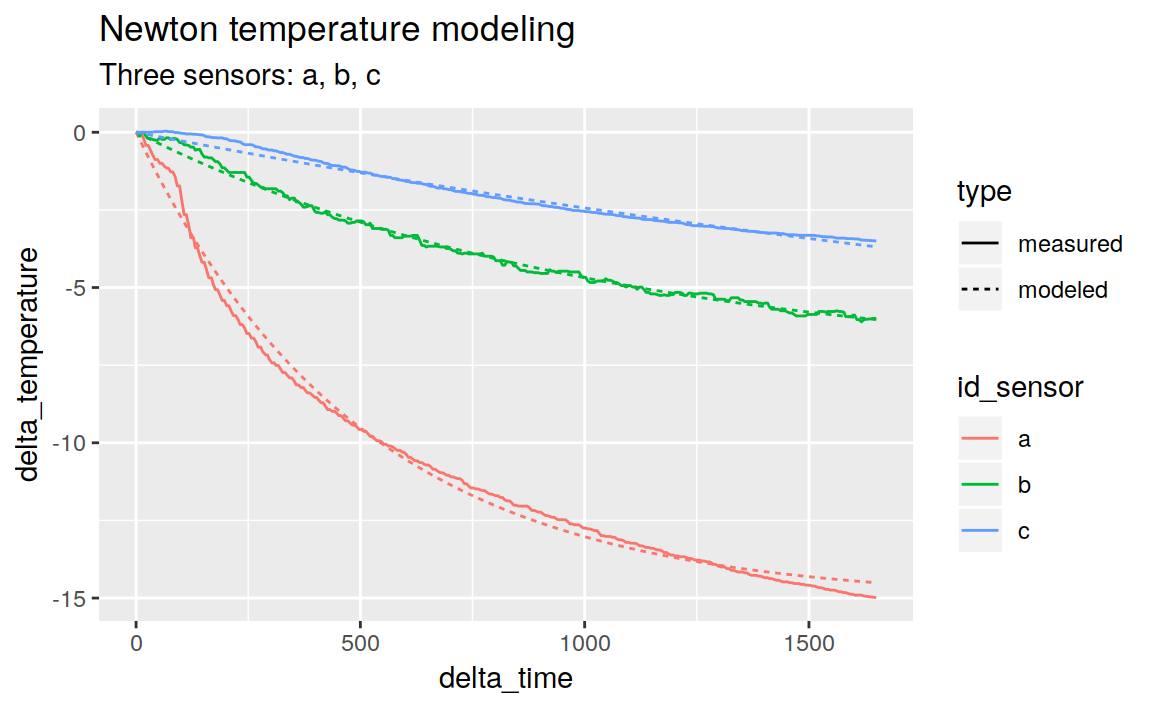
\includegraphics[width=0.7\linewidth]{regression_114-nested_temperature_files/figure-latex/unnamed-chunk-18-1} \end{center}

\hypertarget{apply-multiple-models-on-a-nested-structure}{%
\section{Apply multiple models on a nested structure}\label{apply-multiple-models-on-a-nested-structure}}

\hypertarget{step-1-selection-of-models}{%
\subsection{Step 1: Selection of models}\label{step-1-selection-of-models}}

Make a list of functions to model:

\begin{Shaded}
\begin{Highlighting}[]
\NormalTok{list_model <-}
\StringTok{  }\KeywordTok{list}\NormalTok{(}
    \DataTypeTok{newton_cooling =}\NormalTok{ newton_cooling,}
    \DataTypeTok{semi_infinite_simple =}\NormalTok{ semi_infinite_simple,}
    \DataTypeTok{semi_infinite_convection =}\NormalTok{ semi_infinite_convection}
\NormalTok{  )}
\end{Highlighting}
\end{Shaded}

\hypertarget{step-2-write-a-function-to-define-the-inner-loop}{%
\subsection{Step 2: write a function to define the ``inner'' loop}\label{step-2-write-a-function-to-define-the-inner-loop}}

\begin{Shaded}
\begin{Highlighting}[]
\CommentTok{# add additional variable with the model name}

\NormalTok{fn_model <-}\StringTok{ }\ControlFlowTok{function}\NormalTok{(.model, df) \{}
  \CommentTok{# one parameter for the model in the list, the second for the data}
  \CommentTok{# safer to avoid non-standard evaluation}
  \CommentTok{# df %>% mutate(model = map(data, .model)) }
  
\NormalTok{  df}\OperatorTok{$}\NormalTok{model <-}\StringTok{ }\KeywordTok{map}\NormalTok{(df}\OperatorTok{$}\NormalTok{data, }\KeywordTok{possibly}\NormalTok{(.model, }\OtherTok{NULL}\NormalTok{))}
\NormalTok{  df}
\NormalTok{\}}
\end{Highlighting}
\end{Shaded}

\begin{itemize}
\item
  for a given model-function and a given (weird) data-frame, return a modified version of that data-frame with a column \texttt{model}, which is the model-function applied to each element of the data-frame's \texttt{data} column (which is itself a list of data-frames)
\item
  the purrr functions \texttt{safely()} and \texttt{possibly()} are \textbf{very} interesting. I think they could be useful outside of purrr as a friendlier way to do error-handling.
\end{itemize}

\hypertarget{step-3-use-map_df-to-define-the-outer-loop}{%
\subsection{\texorpdfstring{Step 3: Use \texttt{map\_df()} to define the ``outer'' loop}{Step 3: Use map\_df() to define the ``outer'' loop}}\label{step-3-use-map_df-to-define-the-outer-loop}}

\begin{Shaded}
\begin{Highlighting}[]
\CommentTok{# this dataframe will be the second input of fn_model}
\NormalTok{delta_nested }\OperatorTok\StringTok{ }
\StringTok{  }\KeywordTok{print}\NormalTok{()}
\CommentTok{#> # A tibble: 3 x 2}
\CommentTok{#>   id_sensor data              }
\CommentTok{#>   <chr>     <list>            }
\CommentTok{#> 1 a         <tibble [327 x 2]>}
\CommentTok{#> 2 b         <tibble [327 x 2]>}
\CommentTok{#> 3 c         <tibble [327 x 2]>}
\end{Highlighting}
\end{Shaded}

\begin{Shaded}
\begin{Highlighting}[]
\CommentTok{# fn_model is receiving two inputs: one from list_model and from delta_nested}
\NormalTok{model_nested_new <-}
\StringTok{  }\NormalTok{list_model }\OperatorTok
\StringTok{  }\KeywordTok{map_df}\NormalTok{(fn_model, delta_nested, }\DataTypeTok{.id =} \StringTok{"id_model"}\NormalTok{) }\OperatorTok
\StringTok{  }\KeywordTok{print}\NormalTok{()}
\CommentTok{#> # A tibble: 9 x 4}
\CommentTok{#>   id_model             id_sensor data               model }
\CommentTok{#>   <chr>                <chr>     <list>             <list>}
\CommentTok{#> 1 newton_cooling       a         <tibble [327 x 2]> <nls> }
\CommentTok{#> 2 newton_cooling       b         <tibble [327 x 2]> <nls> }
\CommentTok{#> 3 newton_cooling       c         <tibble [327 x 2]> <nls> }
\CommentTok{#> 4 semi_infinite_simple a         <tibble [327 x 2]> <nls> }
\CommentTok{#> 5 semi_infinite_simple b         <tibble [327 x 2]> <nls> }
\CommentTok{#> 6 semi_infinite_simple c         <tibble [327 x 2]> <nls> }
\CommentTok{#> # ... with 3 more rows}
\end{Highlighting}
\end{Shaded}

\begin{itemize}
\item
  for each element of a list of model-functions, run the inner-loop function, and row-bind the results into a data-frame
\item
  we want to discard the rows where the model failed
\item
  we also want to investigate why they failed, but that's a different talk
\end{itemize}

\hypertarget{step-4-use-map-to-identify-the-null-models}{%
\subsection{\texorpdfstring{Step 4: Use \texttt{map()} to identify the null models}{Step 4: Use map() to identify the null models}}\label{step-4-use-map-to-identify-the-null-models}}

\begin{Shaded}
\begin{Highlighting}[]
\NormalTok{model_nested_new <-}
\StringTok{  }\NormalTok{list_model }\OperatorTok
\StringTok{  }\KeywordTok{map_df}\NormalTok{(fn_model, delta_nested, }\DataTypeTok{.id =} \StringTok{"id_model"}\NormalTok{) }\OperatorTok
\StringTok{  }\KeywordTok{mutate}\NormalTok{(}\DataTypeTok{is_null =} \KeywordTok{map}\NormalTok{(model, is.null)) }\OperatorTok
\StringTok{  }\KeywordTok{print}\NormalTok{()}
\CommentTok{#> # A tibble: 9 x 5}
\CommentTok{#>   id_model             id_sensor data               model  is_null  }
\CommentTok{#>   <chr>                <chr>     <list>             <list> <list>   }
\CommentTok{#> 1 newton_cooling       a         <tibble [327 x 2]> <nls>  <lgl [1]>}
\CommentTok{#> 2 newton_cooling       b         <tibble [327 x 2]> <nls>  <lgl [1]>}
\CommentTok{#> 3 newton_cooling       c         <tibble [327 x 2]> <nls>  <lgl [1]>}
\CommentTok{#> 4 semi_infinite_simple a         <tibble [327 x 2]> <nls>  <lgl [1]>}
\CommentTok{#> 5 semi_infinite_simple b         <tibble [327 x 2]> <nls>  <lgl [1]>}
\CommentTok{#> 6 semi_infinite_simple c         <tibble [327 x 2]> <nls>  <lgl [1]>}
\CommentTok{#> # ... with 3 more rows}
\end{Highlighting}
\end{Shaded}

\begin{itemize}
\tightlist
\item
  using \texttt{map(model,\ is.null)} returns a list column
\item
  to use \texttt{filter()}, we have to escape the weirdness
\end{itemize}

\hypertarget{step-5-map_lgl-to-identify-nulls-and-get-out-of-the-weirdness}{%
\subsection{\texorpdfstring{Step 5: \texttt{map\_lgl()} to identify nulls and get out of the weirdness}{Step 5: map\_lgl() to identify nulls and get out of the weirdness}}\label{step-5-map_lgl-to-identify-nulls-and-get-out-of-the-weirdness}}

\begin{Shaded}
\begin{Highlighting}[]
\NormalTok{model_nested_new <-}
\StringTok{  }\NormalTok{list_model }\OperatorTok
\StringTok{  }\KeywordTok{map_df}\NormalTok{(fn_model, delta_nested, }\DataTypeTok{.id =} \StringTok{"id_model"}\NormalTok{) }\OperatorTok
\StringTok{  }\KeywordTok{mutate}\NormalTok{(}\DataTypeTok{is_null =} \KeywordTok{map_lgl}\NormalTok{(model, is.null)) }\OperatorTok
\StringTok{  }\KeywordTok{print}\NormalTok{()}
\CommentTok{#> # A tibble: 9 x 5}
\CommentTok{#>   id_model             id_sensor data               model  is_null}
\CommentTok{#>   <chr>                <chr>     <list>             <list> <lgl>  }
\CommentTok{#> 1 newton_cooling       a         <tibble [327 x 2]> <nls>  FALSE  }
\CommentTok{#> 2 newton_cooling       b         <tibble [327 x 2]> <nls>  FALSE  }
\CommentTok{#> 3 newton_cooling       c         <tibble [327 x 2]> <nls>  FALSE  }
\CommentTok{#> 4 semi_infinite_simple a         <tibble [327 x 2]> <nls>  FALSE  }
\CommentTok{#> 5 semi_infinite_simple b         <tibble [327 x 2]> <nls>  FALSE  }
\CommentTok{#> 6 semi_infinite_simple c         <tibble [327 x 2]> <nls>  FALSE  }
\CommentTok{#> # ... with 3 more rows}
\end{Highlighting}
\end{Shaded}

\begin{itemize}
\tightlist
\item
  using \texttt{map\_lgl(model,\ is.null)} returns a vector column
\end{itemize}

\hypertarget{step-6-filter-nulls-and-select-variables-to-clean-up}{%
\subsection{\texorpdfstring{Step 6: \texttt{filter()} nulls and \texttt{select()} variables to clean up}{Step 6: filter() nulls and select() variables to clean up}}\label{step-6-filter-nulls-and-select-variables-to-clean-up}}

\begin{Shaded}
\begin{Highlighting}[]
\NormalTok{model_nested_new <-}
\StringTok{  }\NormalTok{list_model }\OperatorTok
\StringTok{  }\KeywordTok{map_df}\NormalTok{(fn_model, delta_nested, }\DataTypeTok{.id =} \StringTok{"id_model"}\NormalTok{) }\OperatorTok
\StringTok{  }\KeywordTok{mutate}\NormalTok{(}\DataTypeTok{is_null =} \KeywordTok{map_lgl}\NormalTok{(model, is.null)) }\OperatorTok
\StringTok{  }\KeywordTok{filter}\NormalTok{(}\OperatorTok{!}\NormalTok{is_null) }\OperatorTok
\StringTok{  }\KeywordTok{select}\NormalTok{(}\OperatorTok{-}\NormalTok{is_null) }\OperatorTok
\StringTok{  }\KeywordTok{print}\NormalTok{()}
\CommentTok{#> # A tibble: 6 x 4}
\CommentTok{#>   id_model             id_sensor data               model }
\CommentTok{#>   <chr>                <chr>     <list>             <list>}
\CommentTok{#> 1 newton_cooling       a         <tibble [327 x 2]> <nls> }
\CommentTok{#> 2 newton_cooling       b         <tibble [327 x 2]> <nls> }
\CommentTok{#> 3 newton_cooling       c         <tibble [327 x 2]> <nls> }
\CommentTok{#> 4 semi_infinite_simple a         <tibble [327 x 2]> <nls> }
\CommentTok{#> 5 semi_infinite_simple b         <tibble [327 x 2]> <nls> }
\CommentTok{#> 6 semi_infinite_simple c         <tibble [327 x 2]> <nls>}
\end{Highlighting}
\end{Shaded}

\hypertarget{step-7-calculate-predictions-on-nested-dataframe}{%
\subsection{Step 7: Calculate predictions on nested dataframe}\label{step-7-calculate-predictions-on-nested-dataframe}}

\begin{Shaded}
\begin{Highlighting}[]
\NormalTok{predict_nested <-}\StringTok{ }
\StringTok{  }\NormalTok{model_nested_new }\OperatorTok
\StringTok{  }\KeywordTok{mutate}\NormalTok{(}\DataTypeTok{pred =} \KeywordTok{map2}\NormalTok{(model, data, predict)) }\OperatorTok
\StringTok{  }\KeywordTok{print}\NormalTok{()}
\CommentTok{#> # A tibble: 6 x 5}
\CommentTok{#>   id_model             id_sensor data               model  pred       }
\CommentTok{#>   <chr>                <chr>     <list>             <list> <list>     }
\CommentTok{#> 1 newton_cooling       a         <tibble [327 x 2]> <nls>  <dbl [327]>}
\CommentTok{#> 2 newton_cooling       b         <tibble [327 x 2]> <nls>  <dbl [327]>}
\CommentTok{#> 3 newton_cooling       c         <tibble [327 x 2]> <nls>  <dbl [327]>}
\CommentTok{#> 4 semi_infinite_simple a         <tibble [327 x 2]> <nls>  <dbl [327]>}
\CommentTok{#> 5 semi_infinite_simple b         <tibble [327 x 2]> <nls>  <dbl [327]>}
\CommentTok{#> 6 semi_infinite_simple c         <tibble [327 x 2]> <nls>  <dbl [327]>}
\end{Highlighting}
\end{Shaded}

\hypertarget{unnest-make-it-tall-and-tidy}{%
\subsection{\texorpdfstring{\texttt{unnest()}, make it tall and tidy}{unnest(), make it tall and tidy}}\label{unnest-make-it-tall-and-tidy}}

\begin{Shaded}
\begin{Highlighting}[]
\NormalTok{predict_tall <-}
\StringTok{  }\NormalTok{predict_nested }\OperatorTok
\StringTok{  }\KeywordTok{unnest}\NormalTok{(data, pred) }\OperatorTok\StringTok{ }
\StringTok{  }\KeywordTok{rename}\NormalTok{(}\DataTypeTok{modeled =}\NormalTok{ pred, }\DataTypeTok{measured =}\NormalTok{ delta_temperature) }\OperatorTok
\StringTok{  }\KeywordTok{gather}\NormalTok{(}\StringTok{"type"}\NormalTok{, }\StringTok{"delta_temperature"}\NormalTok{, modeled, measured) }\OperatorTok
\StringTok{  }\KeywordTok{print}\NormalTok{()}
\CommentTok{#> # A tibble: 3,924 x 5}
\CommentTok{#>   id_model       id_sensor delta_time type    delta_temperature}
\CommentTok{#>   <chr>          <chr>          <dbl> <chr>               <dbl>}
\CommentTok{#> 1 newton_cooling a                  0 modeled             0    }
\CommentTok{#> 2 newton_cooling a                  4 modeled            -0.120}
\CommentTok{#> 3 newton_cooling a                  8 modeled            -0.239}
\CommentTok{#> 4 newton_cooling a                 12 modeled            -0.357}
\CommentTok{#> 5 newton_cooling a                 17 modeled            -0.503}
\CommentTok{#> 6 newton_cooling a                 22 modeled            -0.648}
\CommentTok{#> # ... with 3,918 more rows}
\end{Highlighting}
\end{Shaded}

\hypertarget{visualize-the-predictions}{%
\subsection{Visualize the predictions}\label{visualize-the-predictions}}

\begin{Shaded}
\begin{Highlighting}[]
\NormalTok{predict_tall }\OperatorTok
\StringTok{  }\KeywordTok{ggplot}\NormalTok{(}\KeywordTok{aes}\NormalTok{(}\DataTypeTok{x =}\NormalTok{ delta_time, }\DataTypeTok{y =}\NormalTok{ delta_temperature)) }\OperatorTok{+}
\StringTok{  }\KeywordTok{geom_line}\NormalTok{(}\KeywordTok{aes}\NormalTok{(}\DataTypeTok{color =}\NormalTok{ id_sensor, }\DataTypeTok{linetype =}\NormalTok{ type)) }\OperatorTok{+}
\StringTok{  }\KeywordTok{facet_grid}\NormalTok{(id_model }\OperatorTok{~}\StringTok{ }\NormalTok{.) }\OperatorTok{+}
\StringTok{  }\KeywordTok{labs}\NormalTok{(}\DataTypeTok{title =} \StringTok{"Newton and Semi-infinite temperature modeling"}\NormalTok{, }
       \DataTypeTok{subtitle =} \StringTok{"Three sensors: a, b, c"}\NormalTok{)}
\end{Highlighting}
\end{Shaded}

\begin{center}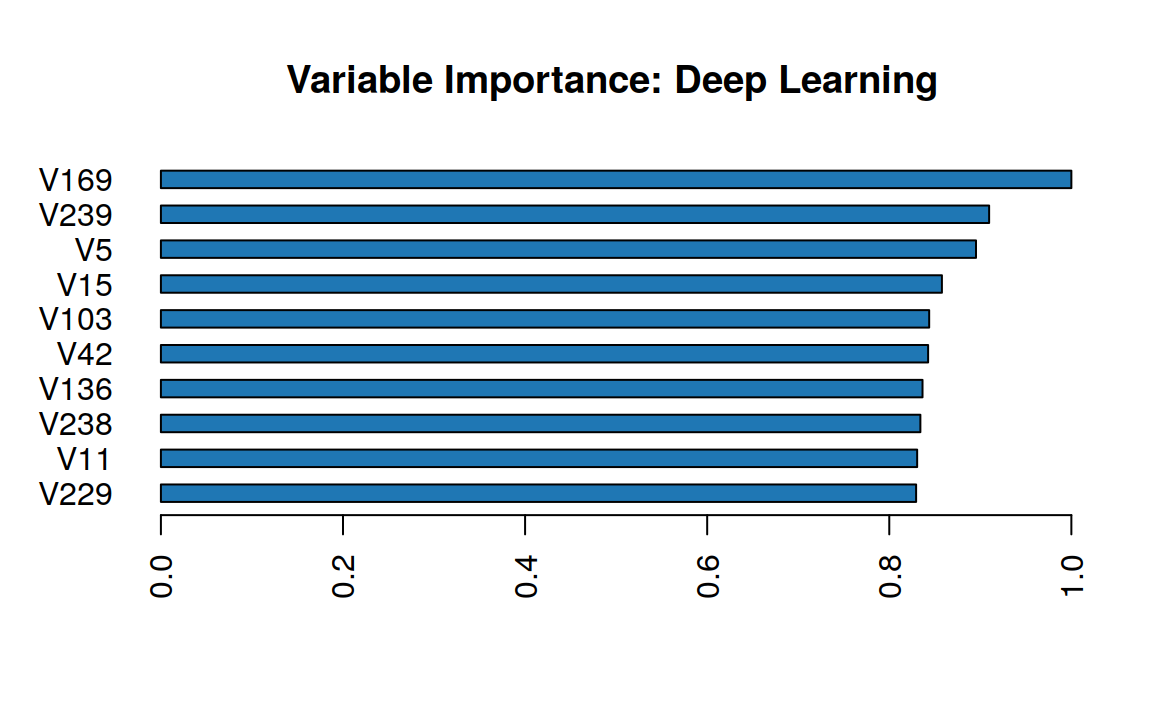
\includegraphics[width=0.7\linewidth]{regression_114-nested_temperature_files/figure-latex/unnamed-chunk-28-1} \end{center}

\hypertarget{lets-get-the-residuals}{%
\subsection{Let's get the residuals}\label{lets-get-the-residuals}}

\begin{Shaded}
\begin{Highlighting}[]
\NormalTok{resid <-}
\StringTok{  }\NormalTok{model_nested_new }\OperatorTok
\StringTok{  }\KeywordTok{mutate}\NormalTok{(}\DataTypeTok{resid =} \KeywordTok{map}\NormalTok{(model, resid)) }\OperatorTok
\StringTok{  }\KeywordTok{unnest}\NormalTok{(data, resid) }\OperatorTok
\StringTok{  }\KeywordTok{print}\NormalTok{()}
\CommentTok{#> # A tibble: 1,962 x 5}
\CommentTok{#>   id_model       id_sensor resid delta_time delta_temperature}
\CommentTok{#>   <chr>          <chr>     <dbl>      <dbl>             <dbl>}
\CommentTok{#> 1 newton_cooling a         0              0             0    }
\CommentTok{#> 2 newton_cooling a         0.120          4             0    }
\CommentTok{#> 3 newton_cooling a         0.179          8            -0.06 }
\CommentTok{#> 4 newton_cooling a         0.297         12            -0.06 }
\CommentTok{#> 5 newton_cooling a         0.292         17            -0.211}
\CommentTok{#> 6 newton_cooling a         0.225         22            -0.423}
\CommentTok{#> # ... with 1,956 more rows}
\end{Highlighting}
\end{Shaded}

\hypertarget{and-visualize-them}{%
\subsection{And visualize them}\label{and-visualize-them}}

\begin{Shaded}
\begin{Highlighting}[]
\NormalTok{resid }\OperatorTok
\StringTok{  }\KeywordTok{ggplot}\NormalTok{(}\KeywordTok{aes}\NormalTok{(}\DataTypeTok{x =}\NormalTok{ delta_time, }\DataTypeTok{y =}\NormalTok{ resid)) }\OperatorTok{+}
\StringTok{  }\KeywordTok{geom_line}\NormalTok{(}\KeywordTok{aes}\NormalTok{(}\DataTypeTok{color =}\NormalTok{ id_sensor)) }\OperatorTok{+}
\StringTok{  }\KeywordTok{facet_grid}\NormalTok{(id_model }\OperatorTok{~}\StringTok{ }\NormalTok{.) }\OperatorTok{+}
\StringTok{  }\KeywordTok{labs}\NormalTok{(}\DataTypeTok{title =} \StringTok{"Residuals for Newton and Semi-infinite models"}\NormalTok{)}
\end{Highlighting}
\end{Shaded}

\begin{center}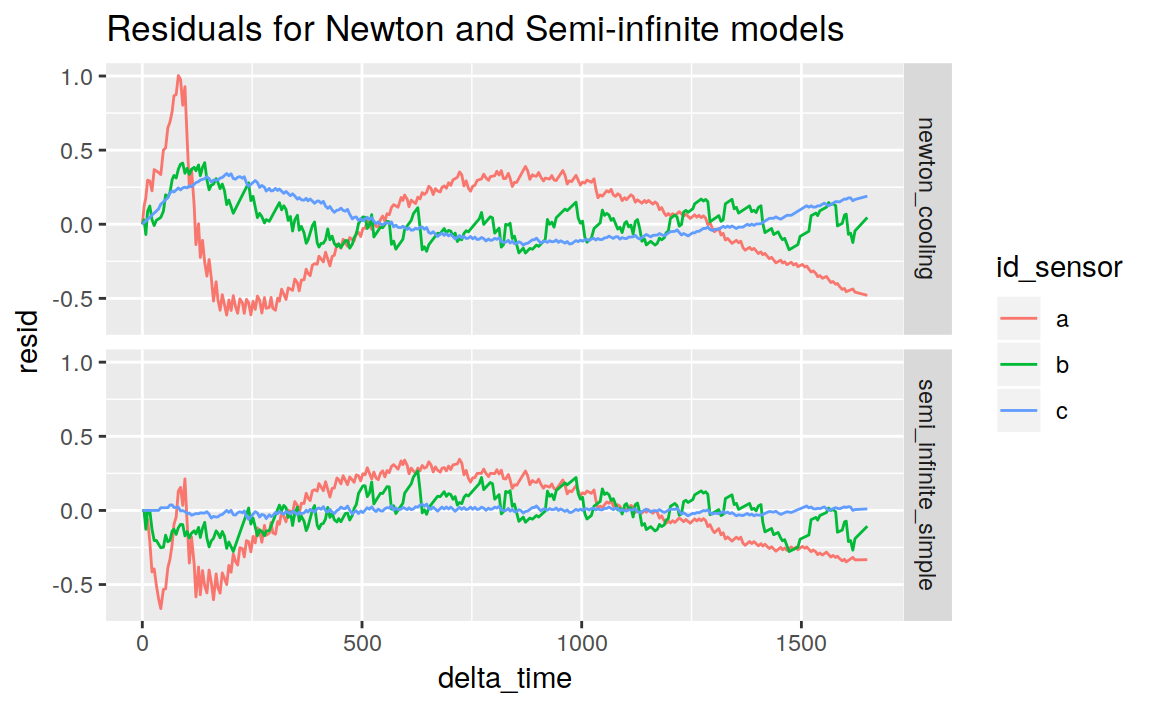
\includegraphics[width=0.7\linewidth]{regression_114-nested_temperature_files/figure-latex/unnamed-chunk-30-1} \end{center}

\hypertarget{using-broom-package-to-look-at-model-statistics}{%
\section{Using broom package to look at model-statistics}\label{using-broom-package-to-look-at-model-statistics}}

We will use a previous defined dataframe with the model and data:

\begin{Shaded}
\begin{Highlighting}[]
\NormalTok{model_nested_new }\OperatorTok\StringTok{ }
\StringTok{  }\KeywordTok{print}\NormalTok{()}
\CommentTok{#> # A tibble: 6 x 4}
\CommentTok{#>   id_model             id_sensor data               model }
\CommentTok{#>   <chr>                <chr>     <list>             <list>}
\CommentTok{#> 1 newton_cooling       a         <tibble [327 x 2]> <nls> }
\CommentTok{#> 2 newton_cooling       b         <tibble [327 x 2]> <nls> }
\CommentTok{#> 3 newton_cooling       c         <tibble [327 x 2]> <nls> }
\CommentTok{#> 4 semi_infinite_simple a         <tibble [327 x 2]> <nls> }
\CommentTok{#> 5 semi_infinite_simple b         <tibble [327 x 2]> <nls> }
\CommentTok{#> 6 semi_infinite_simple c         <tibble [327 x 2]> <nls>}
\end{Highlighting}
\end{Shaded}

The \texttt{tidy()} function extracts statistics from a model.

\begin{Shaded}
\begin{Highlighting}[]
\CommentTok{# apply over model_nested_new but only three variables}
\NormalTok{model_parameters <-}\StringTok{ }
\StringTok{  }\NormalTok{model_nested_new }\OperatorTok
\StringTok{  }\KeywordTok{select}\NormalTok{(id_model, id_sensor, model) }\OperatorTok
\StringTok{  }\KeywordTok{mutate}\NormalTok{(}\DataTypeTok{tidy =} \KeywordTok{map}\NormalTok{(model, tidy)) }\OperatorTok
\StringTok{  }\KeywordTok{select}\NormalTok{(}\OperatorTok{-}\NormalTok{model) }\OperatorTok
\StringTok{  }\KeywordTok{unnest}\NormalTok{() }\OperatorTok
\StringTok{  }\KeywordTok{print}\NormalTok{()}
\CommentTok{#> # A tibble: 12 x 7}
\CommentTok{#>   id_model    id_sensor term         estimate std.error statistic   p.value}
\CommentTok{#>   <chr>       <chr>     <chr>           <dbl>     <dbl>     <dbl>     <dbl>}
\CommentTok{#> 1 newton_coo~ a         delta_tempe~   -15.1     0.0526    -286.  0.       }
\CommentTok{#> 2 newton_coo~ a         tau_0          500.      4.84       103.  1.07e-250}
\CommentTok{#> 3 newton_coo~ b         delta_tempe~    -7.59    0.0676    -112.  6.38e-262}
\CommentTok{#> 4 newton_coo~ b         tau_0         1041.     16.2         64.2 9.05e-187}
\CommentTok{#> 5 newton_coo~ c         delta_tempe~    -9.87    0.704      -14.0 3.16e- 35}
\CommentTok{#> 6 newton_coo~ c         tau_0         3525.    299.          11.8 5.61e- 27}
\CommentTok{#> # ... with 6 more rows}
\end{Highlighting}
\end{Shaded}

\hypertarget{get-a-sense-of-the-coefficients}{%
\subsection{Get a sense of the coefficients}\label{get-a-sense-of-the-coefficients}}

\begin{Shaded}
\begin{Highlighting}[]
\NormalTok{model_summary <-}
\StringTok{  }\NormalTok{model_parameters }\OperatorTok
\StringTok{  }\KeywordTok{select}\NormalTok{(id_model, id_sensor, term, estimate) }\OperatorTok
\StringTok{  }\KeywordTok{spread}\NormalTok{(}\DataTypeTok{key =} \StringTok{"term"}\NormalTok{, }\DataTypeTok{value =} \StringTok{"estimate"}\NormalTok{) }\OperatorTok
\StringTok{  }\KeywordTok{print}\NormalTok{()}
\CommentTok{#> # A tibble: 6 x 4}
\CommentTok{#>   id_model             id_sensor delta_temperature_0 tau_0}
\CommentTok{#>   <chr>                <chr>                   <dbl> <dbl>}
\CommentTok{#> 1 newton_cooling       a                      -15.1   500.}
\CommentTok{#> 2 newton_cooling       b                       -7.59 1041.}
\CommentTok{#> 3 newton_cooling       c                       -9.87 3525.}
\CommentTok{#> 4 semi_infinite_simple a                      -21.5   139.}
\CommentTok{#> 5 semi_infinite_simple b                      -10.6   287.}
\CommentTok{#> 6 semi_infinite_simple c                       -8.04  500.}
\end{Highlighting}
\end{Shaded}

\hypertarget{summary}{%
\subsection{Summary}\label{summary}}

\begin{itemize}
\tightlist
\item
  this is just a smalll part of purrr
\item
  there seem to be parallels between \texttt{tidyr::nest()/purrr::map()} and \texttt{dplyr::group\_by()/dplyr::do()}

  \begin{itemize}
  \tightlist
  \item
    to my mind, the purrr framework is more understandable
  \item
    update tweet from \href{https://twitter.com/hadleywickham/status/719542847045636096}{Hadley}
  \end{itemize}
\end{itemize}

References from Hadley:

\begin{itemize}
\tightlist
\item
  \href{http://blog.rstudio.org/2015/09/29/purrr-0-1-0/}{purrr 0.1.0 announcement}
\item
  \href{http://blog.rstudio.org/2016/01/06/purrr-0-2-0/}{purrr 0.2.0 announcement}
\item
  \href{http://r4ds.had.co.nz/iteration.html}{chapter from Garrett Grolemund and Hadley's forthcoming book}
\end{itemize}

\hypertarget{linear-regression.-world-happiness}{%
\chapter{Linear Regression. World Happiness}\label{linear-regression.-world-happiness}}

\hypertarget{introduction}{%
\section{Introduction}\label{introduction}}

Source: \url{http://enhancedatascience.com/2017/04/25/r-basics-linear-regression-with-r/}
Data: \url{https://www.kaggle.com/unsdsn/world-happiness}

Linear regression is one of the basics of statistics and machine learning. Hence, it is a must-have to know how to perform a linear regression with R and how to interpret the results.

Linear regression algorithm will fit the best straight line that fits the data? To do so, it will minimise the squared distance between the points of the dataset and the fitted line.

For this tutorial, we will use the World Happiness report dataset from Kaggle. This report analyses the Happiness of each country according to several factors such as wealth, health, family life, \ldots{} Our goal will be to find the most important factors of happiness. What a noble goal!

\hypertarget{a-quick-exploration-of-the-data}{%
\section{A quick exploration of the data}\label{a-quick-exploration-of-the-data}}

Before fitting any model, we need to know our data better. First, let's import the data into R. Please download the dataset from Kaggle and put it in your working directory.

The code below imports the data as data.table and clean the column names (a lot of . were appearing in the original ones)

\begin{Shaded}
\begin{Highlighting}[]
\KeywordTok{require}\NormalTok{(data.table)}
\CommentTok{#> Loading required package: data.table}
\NormalTok{data_happiness_dir <-}\StringTok{ }\KeywordTok{file.path}\NormalTok{(data_raw_dir, }\StringTok{"happiness"}\NormalTok{)}

\NormalTok{Happiness_Data =}\StringTok{ }\KeywordTok{data.table}\NormalTok{(}\KeywordTok{read.csv}\NormalTok{(}\KeywordTok{file.path}\NormalTok{(data_happiness_dir, }\StringTok{'2016.csv'}\NormalTok{)))}
\KeywordTok{colnames}\NormalTok{(Happiness_Data) <-}\StringTok{ }\KeywordTok{gsub}\NormalTok{(}\StringTok{'.'}\NormalTok{,}\StringTok{''}\NormalTok{,}\KeywordTok{colnames}\NormalTok{(Happiness_Data), }\DataTypeTok{fixed=}\NormalTok{T)}
\end{Highlighting}
\end{Shaded}

Now, let's plot a Scatter Plot Matrix to get a grasp of how our variables are related one to another. To do so, the GGally package is great.

\begin{Shaded}
\begin{Highlighting}[]
\KeywordTok{require}\NormalTok{(ggplot2)}
\CommentTok{#> Loading required package: ggplot2}
\CommentTok{#> Registered S3 methods overwritten by 'ggplot2':}
\CommentTok{#>   method         from }
\CommentTok{#>   [.quosures     rlang}
\CommentTok{#>   c.quosures     rlang}
\CommentTok{#>   print.quosures rlang}
\KeywordTok{require}\NormalTok{(GGally)}
\CommentTok{#> Loading required package: GGally}
\CommentTok{#> Registered S3 method overwritten by 'GGally':}
\CommentTok{#>   method from   }
\CommentTok{#>   +.gg   ggplot2}
\KeywordTok{ggpairs}\NormalTok{(Happiness_Data[,}\KeywordTok{c}\NormalTok{(}\DecValTok{4}\NormalTok{,}\DecValTok{7}\OperatorTok{:}\DecValTok{13}\NormalTok{), }\DataTypeTok{with=}\NormalTok{F], }\DataTypeTok{lower =} \KeywordTok{list}\NormalTok{( }\DataTypeTok{continuous =} \StringTok{"smooth"}\NormalTok{))}
\end{Highlighting}
\end{Shaded}

\begin{center}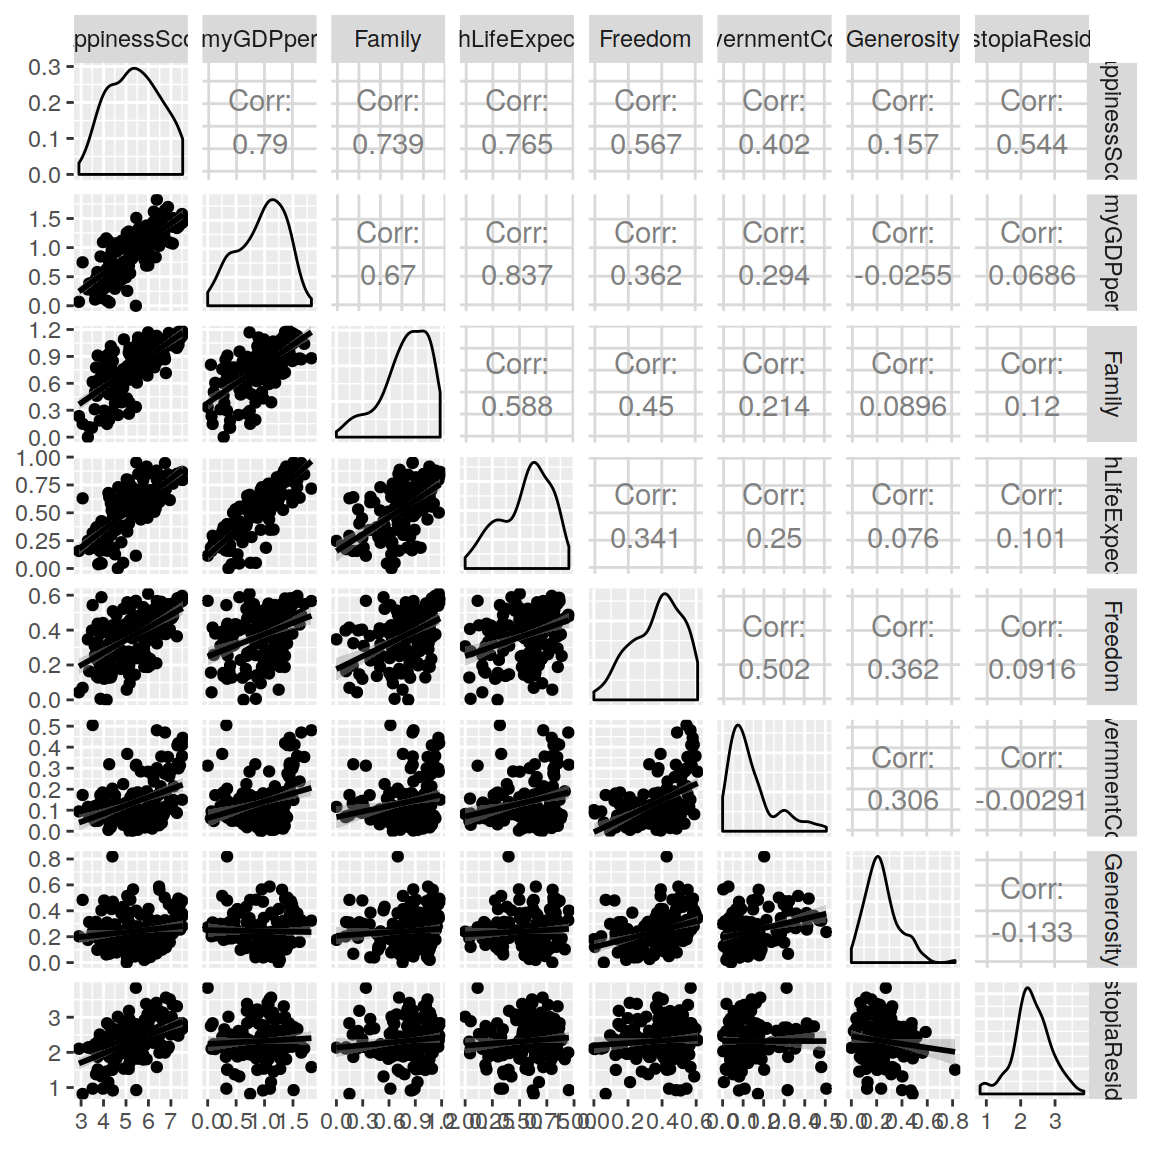
\includegraphics[width=0.7\linewidth]{regression_136-happiness_files/figure-latex/pairplot-1} \end{center}

All the variables are positively correlated with the Happiness score. We can expect that most of the coefficients in the linear regression will be positive. However, the correlation between the variable is often more than 0.5, so we can expect that multicollinearity will appear in the regression.

In the data, we also have access to the Country where the score was computed. Even if it's not useful for the regression, let's plot the data on a map!

\begin{Shaded}
\begin{Highlighting}[]
\KeywordTok{require}\NormalTok{(}\StringTok{'rworldmap'}\NormalTok{)}
\CommentTok{#> Loading required package: rworldmap}
\CommentTok{#> Loading required package: sp}
\CommentTok{#> }\AlertTok{###}\CommentTok{ Welcome to rworldmap }\AlertTok{###}
\CommentTok{#> For a short introduction type :   vignette('rworldmap')}
\KeywordTok{library}\NormalTok{(reshape2)}
\CommentTok{#> }
\CommentTok{#> Attaching package: 'reshape2'}
\CommentTok{#> The following objects are masked from 'package:data.table':}
\CommentTok{#> }
\CommentTok{#>     dcast, melt}

\NormalTok{map.world <-}\StringTok{ }\KeywordTok{map_data}\NormalTok{(}\DataTypeTok{map=}\StringTok{"world"}\NormalTok{)}

\NormalTok{dataPlot<-}\StringTok{ }\KeywordTok{melt}\NormalTok{(Happiness_Data, }\DataTypeTok{id.vars =}\StringTok{'Country'}\NormalTok{, }
                \DataTypeTok{measure.vars =} \KeywordTok{colnames}\NormalTok{(Happiness_Data)[}\KeywordTok{c}\NormalTok{(}\DecValTok{4}\NormalTok{,}\DecValTok{7}\OperatorTok{:}\DecValTok{13}\NormalTok{)])}

\CommentTok{#Correcting names that are different}
\NormalTok{dataPlot[Country }\OperatorTok{==}\StringTok{ 'United States'}\NormalTok{, Country}\OperatorTok{:}\ErrorTok{=}\StringTok{'USA'}\NormalTok{]}
\NormalTok{dataPlot[Country }\OperatorTok{==}\StringTok{ 'United Kingdoms'}\NormalTok{, Country}\OperatorTok{:}\ErrorTok{=}\StringTok{'UK'}\NormalTok{]}

\CommentTok{##Rescaling each variable to have nice gradient}
\NormalTok{dataPlot[,value}\OperatorTok{:}\ErrorTok{=}\NormalTok{value}\OperatorTok{/}\KeywordTok{max}\NormalTok{(value), by=variable]}
\NormalTok{dataMap =}\StringTok{ }\KeywordTok{data.table}\NormalTok{(}\KeywordTok{merge}\NormalTok{(map.world, dataPlot, }
                           \DataTypeTok{by.x=}\StringTok{'region'}\NormalTok{, }
                           \DataTypeTok{by.y=}\StringTok{'Country'}\NormalTok{, }
                           \DataTypeTok{all.x=}\NormalTok{T))}
\NormalTok{dataMap =}\StringTok{ }\NormalTok{dataMap[}\KeywordTok{order}\NormalTok{(order)]}
\NormalTok{dataMap =}\StringTok{ }\NormalTok{dataMap[}\KeywordTok{order}\NormalTok{(order)][}\OperatorTok{!}\KeywordTok{is.na}\NormalTok{(variable)]}
\NormalTok{gg <-}\StringTok{ }\KeywordTok{ggplot}\NormalTok{()}
\NormalTok{gg <-}\StringTok{ }\NormalTok{gg }\OperatorTok{+}\StringTok{ }
\StringTok{    }\KeywordTok{geom_map}\NormalTok{(}\DataTypeTok{data=}\NormalTok{dataMap, }\DataTypeTok{map=}\NormalTok{dataMap, }
             \KeywordTok{aes}\NormalTok{(}\DataTypeTok{map_id =}\NormalTok{ region, }\DataTypeTok{x=}\NormalTok{long, }\DataTypeTok{y=}\NormalTok{lat, }\DataTypeTok{fill=}\NormalTok{value)) }\OperatorTok{+}
\StringTok{    }\CommentTok{# facet_wrap(~variable, scale='free')}
\StringTok{    }\KeywordTok{facet_wrap}\NormalTok{(}\OperatorTok{~}\NormalTok{variable)}
\CommentTok{#> Warning: Ignoring unknown aesthetics: x, y}
\NormalTok{gg <-}\StringTok{ }\NormalTok{gg }\OperatorTok{+}\StringTok{ }\KeywordTok{scale_fill_gradient}\NormalTok{(}\DataTypeTok{low =} \StringTok{"navy"}\NormalTok{, }\DataTypeTok{high =} \StringTok{"lightblue"}\NormalTok{)}
\NormalTok{gg <-}\StringTok{ }\NormalTok{gg }\OperatorTok{+}\StringTok{ }\KeywordTok{coord_equal}\NormalTok{()}
\end{Highlighting}
\end{Shaded}

The code above is a classic code for a map. A few important points:

We reordered the point before plotting to avoid some artefacts.
The merge is a right outer join, all the points of the map need to be kept. Otherwise, points will be missing which will mess up the map.
Each variable is rescaled so that a facet\_wrap can be used. Here, the absolute level of a variable is not of primary interest. This is the relative level of a variable between countries that we want to visualise.

\begin{Shaded}
\begin{Highlighting}[]
\NormalTok{gg}
\end{Highlighting}
\end{Shaded}

\begin{center}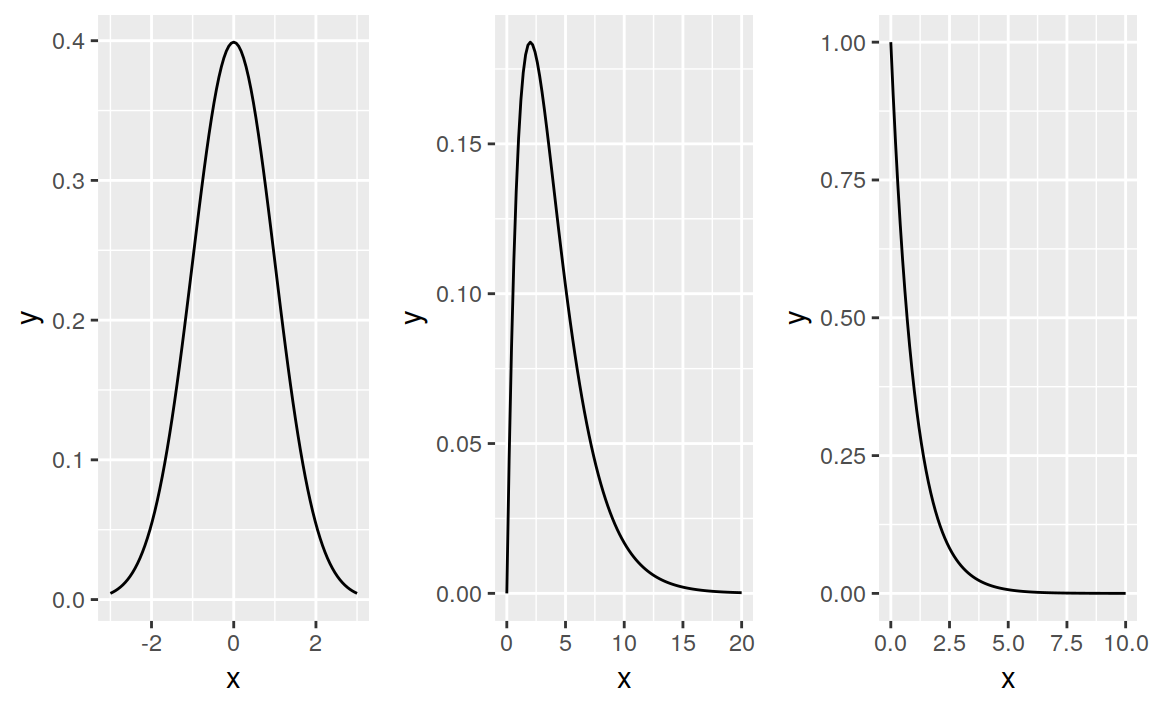
\includegraphics[width=0.7\linewidth]{regression_136-happiness_files/figure-latex/unnamed-chunk-2-1} \end{center}

The distinction between North and South is quite visible. In addition to this, countries that have suffered from the crisis are also really visible.

\hypertarget{linear-regression-with-r}{%
\section{Linear regression with R}\label{linear-regression-with-r}}

Now that we have taken a look at our data, a first model can be fitted. The explanatory variables are the DGP per capita, the life expectancy, the level of freedom and the trust in the government.

\begin{Shaded}
\begin{Highlighting}[]
\CommentTok{##First model}
\NormalTok{model1 <-}\StringTok{ }\KeywordTok{lm}\NormalTok{(HappinessScore }\OperatorTok{~}\StringTok{ }\NormalTok{EconomyGDPperCapita }\OperatorTok{+}\StringTok{ }\NormalTok{Family }\OperatorTok{+}\StringTok{ }
\StringTok{                 }\NormalTok{HealthLifeExpectancy }\OperatorTok{+}\StringTok{ }\NormalTok{Freedom }\OperatorTok{+}\StringTok{ }\NormalTok{TrustGovernmentCorruption, }
             \DataTypeTok{data=}\NormalTok{Happiness_Data)}
\end{Highlighting}
\end{Shaded}

\hypertarget{regression-summary}{%
\section{Regression summary}\label{regression-summary}}

The summary function provides a very easy way to assess a linear regression in R.

\begin{Shaded}
\begin{Highlighting}[]
\KeywordTok{require}\NormalTok{(stargazer)}
\CommentTok{#> Loading required package: stargazer}
\CommentTok{#> }
\CommentTok{#> Please cite as:}
\CommentTok{#>  Hlavac, Marek (2018). stargazer: Well-Formatted Regression and Summary Statistics Tables.}
\CommentTok{#>  R package version 5.2.2. https://CRAN.R-project.org/package=stargazer}

\CommentTok{##Quick summary}
\NormalTok{sum1=}\KeywordTok{summary}\NormalTok{(model1)}
\NormalTok{sum1}
\CommentTok{#> }
\CommentTok{#> Call:}
\CommentTok{#> lm(formula = HappinessScore ~ EconomyGDPperCapita + Family + }
\CommentTok{#>     HealthLifeExpectancy + Freedom + TrustGovernmentCorruption, }
\CommentTok{#>     data = Happiness_Data)}
\CommentTok{#> }
\CommentTok{#> Residuals:}
\CommentTok{#>     Min      1Q  Median      3Q     Max }
\CommentTok{#> -1.4833 -0.2817 -0.0277  0.3280  1.4615 }
\CommentTok{#> }
\CommentTok{#> Coefficients:}
\CommentTok{#>                           Estimate Std. Error t value Pr(>|t|)    }
\CommentTok{#> (Intercept)                  2.212      0.150   14.73  < 2e-16 ***}
\CommentTok{#> EconomyGDPperCapita          0.697      0.209    3.33   0.0011 ** }
\CommentTok{#> Family                       1.234      0.229    5.39  2.6e-07 ***}
\CommentTok{#> HealthLifeExpectancy         1.462      0.343    4.26  3.5e-05 ***}
\CommentTok{#> Freedom                      1.559      0.373    4.18  5.0e-05 ***}
\CommentTok{#> TrustGovernmentCorruption    0.959      0.455    2.11   0.0365 *  }
\CommentTok{#> ---}
\CommentTok{#> Signif. codes:  0 '***' 0.001 '**' 0.01 '*' 0.05 '.' 0.1 ' ' 1}
\CommentTok{#> }
\CommentTok{#> Residual standard error: 0.535 on 151 degrees of freedom}
\CommentTok{#> Multiple R-squared:  0.787,  Adjusted R-squared:  0.78 }
\CommentTok{#> F-statistic:  112 on 5 and 151 DF,  p-value: <2e-16}

\KeywordTok{stargazer}\NormalTok{(model1,}\DataTypeTok{type=}\StringTok{'text'}\NormalTok{)}
\CommentTok{#> }
\CommentTok{#> =====================================================}
\CommentTok{#>                               Dependent variable:    }
\CommentTok{#>                           ---------------------------}
\CommentTok{#>                                 HappinessScore       }
\CommentTok{#> -----------------------------------------------------}
\CommentTok{#> EconomyGDPperCapita                0.697***          }
\CommentTok{#>                                     (0.209)          }
\CommentTok{#>                                                      }
\CommentTok{#> Family                             1.230***          }
\CommentTok{#>                                     (0.229)          }
\CommentTok{#>                                                      }
\CommentTok{#> HealthLifeExpectancy               1.460***          }
\CommentTok{#>                                     (0.343)          }
\CommentTok{#>                                                      }
\CommentTok{#> Freedom                            1.560***          }
\CommentTok{#>                                     (0.373)          }
\CommentTok{#>                                                      }
\CommentTok{#> TrustGovernmentCorruption           0.959**          }
\CommentTok{#>                                     (0.455)          }
\CommentTok{#>                                                      }
\CommentTok{#> Constant                           2.210***          }
\CommentTok{#>                                     (0.150)          }
\CommentTok{#>                                                      }
\CommentTok{#> -----------------------------------------------------}
\CommentTok{#> Observations                          157            }
\CommentTok{#> R2                                   0.787           }
\CommentTok{#> Adjusted R2                          0.780           }
\CommentTok{#> Residual Std. Error            0.535 (df = 151)      }
\CommentTok{#> F Statistic                112.000*** (df = 5; 151)  }
\CommentTok{#> =====================================================}
\CommentTok{#> Note:                     *p<0.1; **p<0.05; ***p<0.01}
\end{Highlighting}
\end{Shaded}

A quick interpretation:

\begin{itemize}
\tightlist
\item
  All the coefficient are significative at a .05 threshold
\item
  The overall model is also significative
\item
  It explains 78.7\% of Happiness in the dataset
\item
  As expected all the relationship between the explanatory variables and the output variable are positives.
\end{itemize}

The model is doing well!

You can also easily get a given indicator of the model performance, such as R², the different coefficients or the p-value of the overall model.

\begin{Shaded}
\begin{Highlighting}[]
\CommentTok{##R²}
\NormalTok{sum1}\OperatorTok{$}\NormalTok{r.squared}\OperatorTok{*}\DecValTok{100}
\CommentTok{#> [1] 78.7}
\CommentTok{##Coefficients}
\NormalTok{sum1}\OperatorTok{$}\NormalTok{coefficients}
\CommentTok{#>                           Estimate Std. Error t value Pr(>|t|)}
\CommentTok{#> (Intercept)                  2.212      0.150   14.73 5.20e-31}
\CommentTok{#> EconomyGDPperCapita          0.697      0.209    3.33 1.10e-03}
\CommentTok{#> Family                       1.234      0.229    5.39 2.62e-07}
\CommentTok{#> HealthLifeExpectancy         1.462      0.343    4.26 3.53e-05}
\CommentTok{#> Freedom                      1.559      0.373    4.18 5.01e-05}
\CommentTok{#> TrustGovernmentCorruption    0.959      0.455    2.11 3.65e-02}
\CommentTok{##p-value}
\KeywordTok{df}\NormalTok{(sum1}\OperatorTok{$}\NormalTok{fstatistic[}\DecValTok{1}\NormalTok{],sum1}\OperatorTok{$}\NormalTok{fstatistic[}\DecValTok{2}\NormalTok{],sum1}\OperatorTok{$}\NormalTok{fstatistic[}\DecValTok{3}\NormalTok{])}
\CommentTok{#>    value }
\CommentTok{#> 3.39e-49}
 
\CommentTok{##Confidence interval of the coefficient}
\KeywordTok{confint}\NormalTok{(model1,}\DataTypeTok{level =} \FloatTok{0.95}\NormalTok{)}
\CommentTok{#>                            2.5 % 97.5 %}
\CommentTok{#> (Intercept)               1.9152   2.51}
\CommentTok{#> EconomyGDPperCapita       0.2833   1.11}
\CommentTok{#> Family                    0.7821   1.69}
\CommentTok{#> HealthLifeExpectancy      0.7846   2.14}
\CommentTok{#> Freedom                   0.8212   2.30}
\CommentTok{#> TrustGovernmentCorruption 0.0609   1.86}
\KeywordTok{confint}\NormalTok{(model1,}\DataTypeTok{level =} \FloatTok{0.99}\NormalTok{)}
\CommentTok{#>                            0.5 % 99.5 %}
\CommentTok{#> (Intercept)                1.820   2.60}
\CommentTok{#> EconomyGDPperCapita        0.151   1.24}
\CommentTok{#> Family                     0.637   1.83}
\CommentTok{#> HealthLifeExpectancy       0.568   2.36}
\CommentTok{#> Freedom                    0.585   2.53}
\CommentTok{#> TrustGovernmentCorruption -0.227   2.14}
\KeywordTok{confint}\NormalTok{(model1,}\DataTypeTok{level =} \FloatTok{0.90}\NormalTok{)}
\CommentTok{#>                             5 % 95 %}
\CommentTok{#> (Intercept)               1.963 2.46}
\CommentTok{#> EconomyGDPperCapita       0.350 1.04}
\CommentTok{#> Family                    0.856 1.61}
\CommentTok{#> HealthLifeExpectancy      0.895 2.03}
\CommentTok{#> Freedom                   0.941 2.18}
\CommentTok{#> TrustGovernmentCorruption 0.207 1.71}
\end{Highlighting}
\end{Shaded}

\hypertarget{regression-analysis}{%
\section{Regression analysis}\label{regression-analysis}}

\hypertarget{residual-analysis}{%
\subsection{Residual analysis}\label{residual-analysis}}

Now that the regression has been done, the analysis and validity of the result can be analysed. Let's begin with residuals and the assumption of normality and homoscedasticity.

\begin{Shaded}
\begin{Highlighting}[]
\CommentTok{# Visualisation of residuals}
\KeywordTok{ggplot}\NormalTok{(model1, }\KeywordTok{aes}\NormalTok{(model1}\OperatorTok{$}\NormalTok{residuals)) }\OperatorTok{+}\StringTok{ }
\StringTok{    }\KeywordTok{geom_histogram}\NormalTok{(}\DataTypeTok{bins=}\DecValTok{20}\NormalTok{, }\KeywordTok{aes}\NormalTok{(}\DataTypeTok{y =}\NormalTok{ ..density..)) }\OperatorTok{+}\StringTok{ }
\StringTok{    }\KeywordTok{geom_density}\NormalTok{(}\DataTypeTok{color=}\StringTok{'blue'}\NormalTok{, }\DataTypeTok{fill =} \StringTok{'blue'}\NormalTok{, }\DataTypeTok{alpha =} \FloatTok{0.2}\NormalTok{) }\OperatorTok{+}\StringTok{ }
\StringTok{    }\KeywordTok{geom_vline}\NormalTok{(}\DataTypeTok{xintercept =} \KeywordTok{mean}\NormalTok{(model1}\OperatorTok{$}\NormalTok{residuals), }\DataTypeTok{color=}\StringTok{'red'}\NormalTok{) }\OperatorTok{+}\StringTok{ }
\StringTok{    }\KeywordTok{stat_function}\NormalTok{(}\DataTypeTok{fun=}\NormalTok{dnorm, }\DataTypeTok{color=}\StringTok{"red"}\NormalTok{, }\DataTypeTok{size=}\DecValTok{1}\NormalTok{, }
                  \DataTypeTok{args =} \KeywordTok{list}\NormalTok{(}\DataTypeTok{mean =} \KeywordTok{mean}\NormalTok{(model1}\OperatorTok{$}\NormalTok{residuals), }
                            \DataTypeTok{sd =} \KeywordTok{sd}\NormalTok{(model1}\OperatorTok{$}\NormalTok{residuals))) }\OperatorTok{+}\StringTok{ }
\StringTok{    }\KeywordTok{xlab}\NormalTok{(}\StringTok{'residuals values'}\NormalTok{)}
\end{Highlighting}
\end{Shaded}

\begin{center}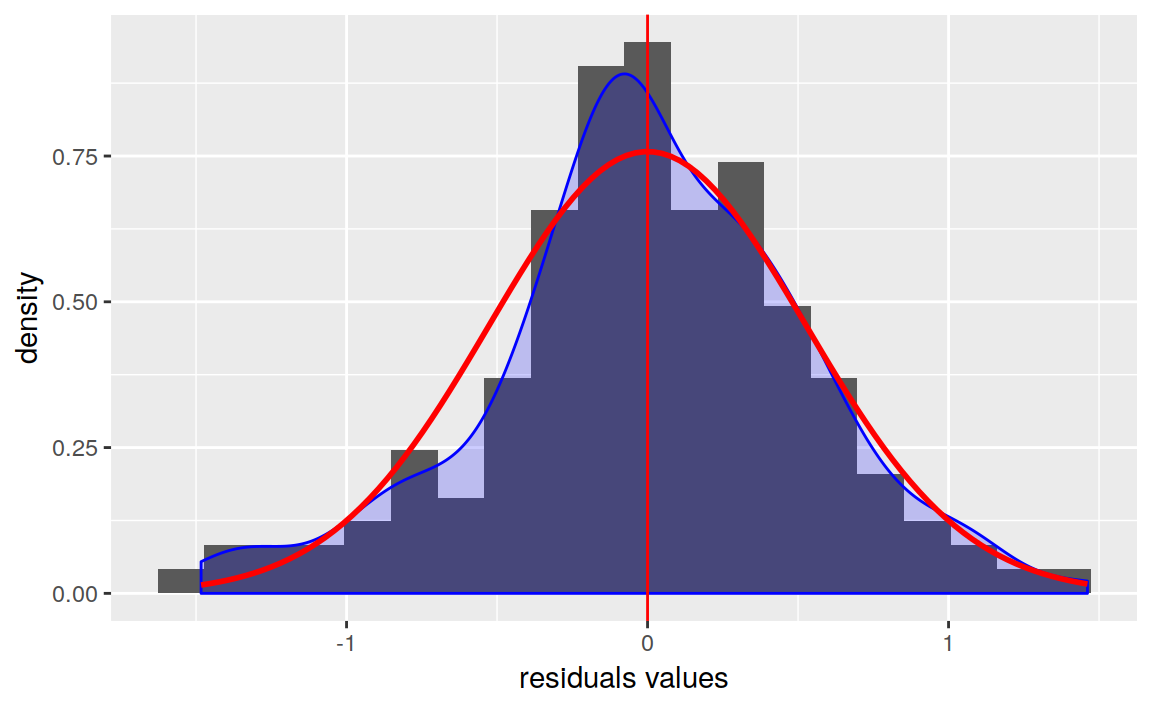
\includegraphics[width=0.7\linewidth]{regression_136-happiness_files/figure-latex/normal-curve-1} \end{center}

The residual versus fitted plot is used to see if the residuals behave the same for the different value of the output (i.e, they have the same variance and mean). The plot shows no strong evidence of heteroscedasticity.

\begin{Shaded}
\begin{Highlighting}[]
\KeywordTok{ggplot}\NormalTok{(model1, }\KeywordTok{aes}\NormalTok{(model1}\OperatorTok{$}\NormalTok{fitted.values, model1}\OperatorTok{$}\NormalTok{residuals)) }\OperatorTok{+}\StringTok{ }
\StringTok{    }\KeywordTok{geom_point}\NormalTok{() }\OperatorTok{+}\StringTok{ }
\StringTok{    }\KeywordTok{geom_hline}\NormalTok{(}\DataTypeTok{yintercept =} \KeywordTok{c}\NormalTok{(}\FloatTok{1.96} \OperatorTok{*}\StringTok{ }\KeywordTok{sd}\NormalTok{(model1}\OperatorTok{$}\NormalTok{residuals), }
                              \OperatorTok{-}\StringTok{ }\FloatTok{1.96} \OperatorTok{*}\StringTok{ }\KeywordTok{sd}\NormalTok{(model1}\OperatorTok{$}\NormalTok{residuals)), }\DataTypeTok{color=}\StringTok{'red'}\NormalTok{) }\OperatorTok{+}\StringTok{ }
\StringTok{    }\KeywordTok{xlab}\NormalTok{(}\StringTok{'fitted value'}\NormalTok{) }\OperatorTok{+}\StringTok{ }
\StringTok{    }\KeywordTok{ylab}\NormalTok{(}\StringTok{'residuals values'}\NormalTok{)}
\end{Highlighting}
\end{Shaded}

\begin{center}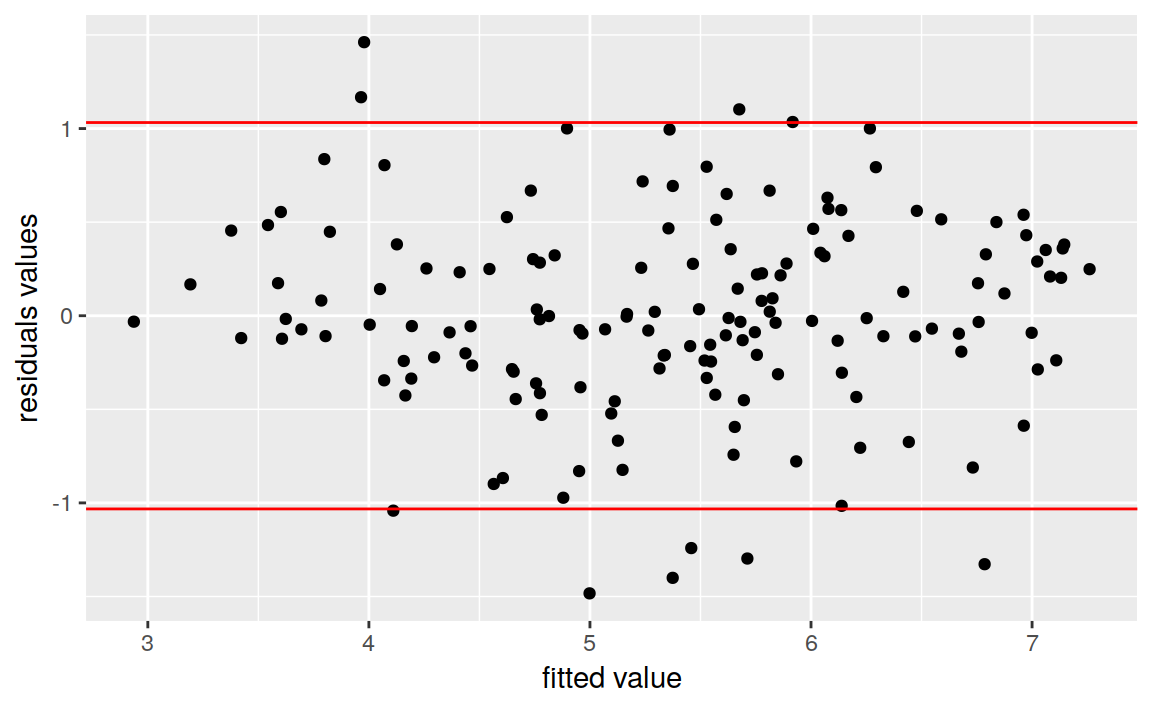
\includegraphics[width=0.7\linewidth]{regression_136-happiness_files/figure-latex/residuals-vs-fitted-1} \end{center}

\hypertarget{analysis-of-colinearity}{%
\section{Analysis of colinearity}\label{analysis-of-colinearity}}

The colinearity can be assessed using VIF, the car package provides a function to compute it directly.

\begin{Shaded}
\begin{Highlighting}[]
\KeywordTok{require}\NormalTok{(}\StringTok{'car'}\NormalTok{)}
\CommentTok{#> Loading required package: car}
\CommentTok{#> Loading required package: carData}
\KeywordTok{vif}\NormalTok{(model1)}
\CommentTok{#>       EconomyGDPperCapita                    Family }
\CommentTok{#>                      4.07                      2.03 }
\CommentTok{#>      HealthLifeExpectancy                   Freedom }
\CommentTok{#>                      3.37                      1.61 }
\CommentTok{#> TrustGovernmentCorruption }
\CommentTok{#>                      1.39}
\end{Highlighting}
\end{Shaded}

All the VIF are less than 5, and hence there is no sign of colinearity.

\hypertarget{what-drives-happiness}{%
\section{What drives happiness}\label{what-drives-happiness}}

Now let's compute standardised betas to see what really drives happiness.

\begin{Shaded}
\begin{Highlighting}[]
\CommentTok{##Standardized betas}
\NormalTok{std_betas =}\StringTok{ }\NormalTok{sum1}\OperatorTok{$}\NormalTok{coefficients[}\OperatorTok{-}\DecValTok{1}\NormalTok{,}\DecValTok{1}\NormalTok{] }\OperatorTok{*}\StringTok{ }
\StringTok{    }\KeywordTok{data.table}\NormalTok{(model1}\OperatorTok{$}\NormalTok{model)[, }\KeywordTok{lapply}\NormalTok{(.SD, sd), .SDcols=}\DecValTok{2}\OperatorTok{:}\DecValTok{6}\NormalTok{] }\OperatorTok{/}\StringTok{ }
\StringTok{    }\KeywordTok{sd}\NormalTok{(model1}\OperatorTok{$}\NormalTok{model}\OperatorTok{$}\NormalTok{HappinessScore)}

\NormalTok{std_betas}
\CommentTok{#>    EconomyGDPperCapita Family HealthLifeExpectancy Freedom}
\CommentTok{#> 1:               0.252  0.288                0.294   0.199}
\CommentTok{#>    TrustGovernmentCorruption}
\CommentTok{#> 1:                    0.0933}
\end{Highlighting}
\end{Shaded}

Though the code above may seem complicated, it is just computing the standardised betas for all variables \texttt{std\_beta=beta*sd(x)/sd(y)}.

The top three coefficients are \textbf{Health and Life expectancy}, \textbf{Family} and \textbf{GDP per Capita}. Though money does not make happiness it is among the top three factors of Happiness!

Now you know how to perform a linear regression with R!

\hypertarget{linear-regression-on-advertising}{%
\chapter{Linear Regression on Advertising}\label{linear-regression-on-advertising}}

Videos, slides:

\begin{itemize}
\tightlist
\item
  \url{https://www.r-bloggers.com/in-depth-introduction-to-machine-learning-in-15-hours-of-expert-videos/}
\end{itemize}

Data:

\begin{itemize}
\tightlist
\item
  \url{http://www-bcf.usc.edu/~gareth/ISL/Advertising.csv}
\end{itemize}

code:

\begin{itemize}
\tightlist
\item
  \url{http://subasish.github.io/pages/ISLwithR/}
\item
  \url{http://math480-s15-zarringhalam.wikispaces.umb.edu/R+Code}
\item
  \url{https://github.com/yahwes/ISLR}
\item
  \url{https://www.tau.ac.il/~saharon/IntroStatLearn.html}
\item
  \url{https://www.waxworksmath.com/Authors/G_M/James/WWW/chapter_3.html}
\item
  \url{https://github.com/asadoughi/stat-learning}
\end{itemize}

plots:

\begin{itemize}
\tightlist
\item
  \url{https://onlinecourses.science.psu.edu/stat857/node/28/}
\end{itemize}

\begin{Shaded}
\begin{Highlighting}[]
\KeywordTok{library}\NormalTok{(readr)}

\NormalTok{advertising <-}\StringTok{ }\KeywordTok{read_csv}\NormalTok{(}\KeywordTok{file.path}\NormalTok{(data_raw_dir, }\StringTok{"Advertising.csv"}\NormalTok{))}
\CommentTok{#> Warning: Missing column names filled in: 'X1' [1]}
\CommentTok{#> Parsed with column specification:}
\CommentTok{#> cols(}
\CommentTok{#>   X1 = col_double(),}
\CommentTok{#>   TV = col_double(),}
\CommentTok{#>   radio = col_double(),}
\CommentTok{#>   newspaper = col_double(),}
\CommentTok{#>   sales = col_double()}
\CommentTok{#> )}
\NormalTok{advertising}
\CommentTok{#> # A tibble: 200 x 5}
\CommentTok{#>      X1    TV radio newspaper sales}
\CommentTok{#>   <dbl> <dbl> <dbl>     <dbl> <dbl>}
\CommentTok{#> 1     1 230.   37.8      69.2  22.1}
\CommentTok{#> 2     2  44.5  39.3      45.1  10.4}
\CommentTok{#> 3     3  17.2  45.9      69.3   9.3}
\CommentTok{#> 4     4 152.   41.3      58.5  18.5}
\CommentTok{#> 5     5 181.   10.8      58.4  12.9}
\CommentTok{#> 6     6   8.7  48.9      75     7.2}
\CommentTok{#> # ... with 194 more rows}
\end{Highlighting}
\end{Shaded}

The Advertising data set. The plot displays sales, in thousands
of units, as a function of TV, radio, and newspaper budgets, in thousands of
dollars, for 200 different markets.

\begin{Shaded}
\begin{Highlighting}[]
\KeywordTok{par}\NormalTok{(}\DataTypeTok{mfrow=}\KeywordTok{c}\NormalTok{(}\DecValTok{1}\NormalTok{,}\DecValTok{3}\NormalTok{))}
\KeywordTok{plot}\NormalTok{(advertising}\OperatorTok{$}\NormalTok{TV, advertising}\OperatorTok{$}\NormalTok{sales, }\DataTypeTok{xlab =} \StringTok{"TV"}\NormalTok{, }\DataTypeTok{ylab =} \StringTok{"Sales"}\NormalTok{, }\DataTypeTok{col =} \StringTok{"red"}\NormalTok{)}
\KeywordTok{plot}\NormalTok{(advertising}\OperatorTok{$}\NormalTok{radio, advertising}\OperatorTok{$}\NormalTok{sales, }\DataTypeTok{xlab=}\StringTok{"Radio"}\NormalTok{, }\DataTypeTok{ylab=}\StringTok{"Sales"}\NormalTok{, }\DataTypeTok{col=}\StringTok{"red"}\NormalTok{)}
\KeywordTok{plot}\NormalTok{(advertising}\OperatorTok{$}\NormalTok{radio, advertising}\OperatorTok{$}\NormalTok{newspaper, }\DataTypeTok{xlab=}\StringTok{"Newspaper"}\NormalTok{, }
     \DataTypeTok{ylab=}\StringTok{"Sales"}\NormalTok{, }\DataTypeTok{col=}\StringTok{"red"}\NormalTok{)}
\end{Highlighting}
\end{Shaded}

\begin{center}\includegraphics[width=0.7\linewidth]{regression_138-advertising_files/figure-latex/unnamed-chunk-3-1} \end{center}

In each plot we show the simple least squares
fit of sales to that variable, as described in Chapter 3. In other words, each blue
line represents a simple model that can be used to predict sales using TV, radio,
and newspaper, respectively.

\begin{Shaded}
\begin{Highlighting}[]
\KeywordTok{par}\NormalTok{(}\DataTypeTok{mfrow=}\KeywordTok{c}\NormalTok{(}\DecValTok{1}\NormalTok{,}\DecValTok{3}\NormalTok{))}
\NormalTok{tv_model <-}\StringTok{ }\KeywordTok{lm}\NormalTok{(sales }\OperatorTok{~}\StringTok{ }\NormalTok{TV, }\DataTypeTok{data =}\NormalTok{ advertising)}
\NormalTok{radio_model <-}\StringTok{ }\KeywordTok{lm}\NormalTok{(sales }\OperatorTok{~}\StringTok{ }\NormalTok{radio, }\DataTypeTok{data =}\NormalTok{ advertising)}
\NormalTok{newspaper_model <-}\StringTok{ }\KeywordTok{lm}\NormalTok{(sales }\OperatorTok{~}\StringTok{ }\NormalTok{newspaper, }\DataTypeTok{data =}\NormalTok{ advertising)}

\KeywordTok{plot}\NormalTok{(advertising}\OperatorTok{$}\NormalTok{TV, advertising}\OperatorTok{$}\NormalTok{sales, }\DataTypeTok{xlab =} \StringTok{"TV"}\NormalTok{, }\DataTypeTok{ylab =} \StringTok{"Sales"}\NormalTok{, }\DataTypeTok{col =} \StringTok{"red"}\NormalTok{)}
\KeywordTok{abline}\NormalTok{(tv_model, }\DataTypeTok{col =} \StringTok{"blue"}\NormalTok{)}
\KeywordTok{plot}\NormalTok{(advertising}\OperatorTok{$}\NormalTok{radio, advertising}\OperatorTok{$}\NormalTok{sales, }\DataTypeTok{xlab=}\StringTok{"Radio"}\NormalTok{, }\DataTypeTok{ylab=}\StringTok{"Sales"}\NormalTok{, }\DataTypeTok{col=}\StringTok{"red"}\NormalTok{)}
\KeywordTok{abline}\NormalTok{(radio_model)}
\KeywordTok{plot}\NormalTok{(advertising}\OperatorTok{$}\NormalTok{newspaper, advertising}\OperatorTok{$}\NormalTok{sales, }\DataTypeTok{xlab=}\StringTok{"Newspaper"}\NormalTok{, }
     \DataTypeTok{ylab=}\StringTok{"Sales"}\NormalTok{, }\DataTypeTok{col=}\StringTok{"red"}\NormalTok{)}
\KeywordTok{abline}\NormalTok{(newspaper_model)}
\end{Highlighting}
\end{Shaded}

\begin{center}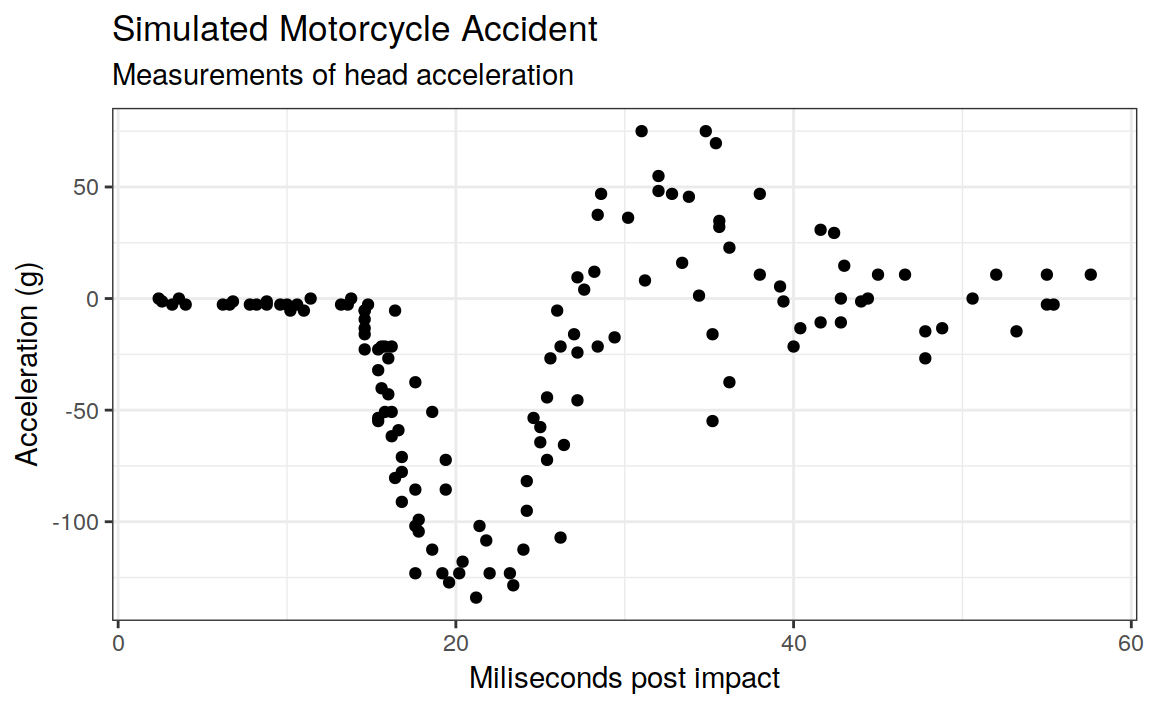
\includegraphics[width=0.7\linewidth]{regression_138-advertising_files/figure-latex/unnamed-chunk-4-1} \end{center}

Recall the Advertising data from Chapter 2. Figure 2.1 displays sales
(in thousands of units) for a particular product as a function of advertis-
ing budgets (in thousands of dollars) for TV, radio, and newspaper media.
Suppose that in our role as statistical consultants we are asked to suggest,
on the basis of this data, a marketing plan for next year that will result in
high product sales. What information would be useful in order to provide
such a recommendation? Here are a few important questions that we might
seek to address:

\begin{enumerate}
\def\labelenumi{\arabic{enumi}.}
\item
  Is there a relationship between advertising budget and sales?
\item
  How strong is the relationship between advertising budget and sales?
\item
  Which media contribute to sales?
\item
  How accurately can we estimate the effect of each medium on sales?
\end{enumerate}

For the Advertising data, the least squares fit for the regression
of sales onto TV is shown. The fit is found by minimizing the sum of squared
errors. Each grey line segment represents an error, and the fit makes a compro-
mise by averaging their squares. In this case a linear fit captures the essence of
the relationship, although it is somewhat deficient in the left of the plot.

\begin{Shaded}
\begin{Highlighting}[]
\NormalTok{tv_model <-}\StringTok{ }\KeywordTok{lm}\NormalTok{(sales }\OperatorTok{~}\StringTok{ }\NormalTok{TV, }\DataTypeTok{data =}\NormalTok{ advertising)}
\KeywordTok{plot}\NormalTok{(advertising}\OperatorTok{$}\NormalTok{TV, advertising}\OperatorTok{$}\NormalTok{sales, }\DataTypeTok{xlab =} \StringTok{"TV"}\NormalTok{, }\DataTypeTok{ylab =} \StringTok{"Sales"}\NormalTok{, }
     \DataTypeTok{col =} \StringTok{"red"}\NormalTok{, }\DataTypeTok{pch=}\DecValTok{16}\NormalTok{)}
\KeywordTok{abline}\NormalTok{(tv_model, }\DataTypeTok{col =} \StringTok{"blue"}\NormalTok{, }\DataTypeTok{lwd=}\DecValTok{2}\NormalTok{)}
\KeywordTok{segments}\NormalTok{(advertising}\OperatorTok{$}\NormalTok{TV, advertising}\OperatorTok{$}\NormalTok{sales, advertising}\OperatorTok{$}\NormalTok{TV, }\KeywordTok{predict}\NormalTok{(tv_model), }
         \DataTypeTok{col =} \StringTok{"gray"}\NormalTok{)}
\end{Highlighting}
\end{Shaded}

\begin{center}\includegraphics[width=0.7\linewidth]{regression_138-advertising_files/figure-latex/unnamed-chunk-5-1} \end{center}

\begin{Shaded}
\begin{Highlighting}[]
\NormalTok{smry <-}\StringTok{ }\KeywordTok{summary}\NormalTok{(tv_model)}
\NormalTok{smry}
\CommentTok{#> }
\CommentTok{#> Call:}
\CommentTok{#> lm(formula = sales ~ TV, data = advertising)}
\CommentTok{#> }
\CommentTok{#> Residuals:}
\CommentTok{#>    Min     1Q Median     3Q    Max }
\CommentTok{#> -8.386 -1.955 -0.191  2.067  7.212 }
\CommentTok{#> }
\CommentTok{#> Coefficients:}
\CommentTok{#>             Estimate Std. Error t value Pr(>|t|)    }
\CommentTok{#> (Intercept)  7.03259    0.45784    15.4   <2e-16 ***}
\CommentTok{#> TV           0.04754    0.00269    17.7   <2e-16 ***}
\CommentTok{#> ---}
\CommentTok{#> Signif. codes:  0 '***' 0.001 '**' 0.01 '*' 0.05 '.' 0.1 ' ' 1}
\CommentTok{#> }
\CommentTok{#> Residual standard error: 3.26 on 198 degrees of freedom}
\CommentTok{#> Multiple R-squared:  0.612,  Adjusted R-squared:  0.61 }
\CommentTok{#> F-statistic:  312 on 1 and 198 DF,  p-value: <2e-16}
\end{Highlighting}
\end{Shaded}

\begin{Shaded}
\begin{Highlighting}[]
\KeywordTok{library}\NormalTok{(lattice)}

\NormalTok{minRss <-}\StringTok{ }\KeywordTok{sqrt}\NormalTok{(}\KeywordTok{abs}\NormalTok{(}\KeywordTok{min}\NormalTok{(smry}\OperatorTok{$}\NormalTok{residuals))) }\OperatorTok{*}\StringTok{ }\KeywordTok{sign}\NormalTok{(}\KeywordTok{min}\NormalTok{(smry}\OperatorTok{$}\NormalTok{residuals))}
\NormalTok{maxRss <-}\StringTok{ }\KeywordTok{sqrt}\NormalTok{(}\KeywordTok{max}\NormalTok{(smry}\OperatorTok{$}\NormalTok{residuals))}

\NormalTok{twovar <-}\StringTok{ }\ControlFlowTok{function}\NormalTok{(x, y) \{ }
\NormalTok{  x}\OperatorTok{^}\DecValTok{2} \OperatorTok{+}\StringTok{ }\NormalTok{y}\OperatorTok{^}\DecValTok{2}\NormalTok{ \}}

\NormalTok{mat <-}\StringTok{ }\KeywordTok{outer}\NormalTok{( }\KeywordTok{seq}\NormalTok{(minRss, maxRss, }\DataTypeTok{length =} \DecValTok{100}\NormalTok{),  }
                \KeywordTok{seq}\NormalTok{(minRss, maxRss, }\DataTypeTok{length =} \DecValTok{100}\NormalTok{), }
                \KeywordTok{Vectorize}\NormalTok{( }\ControlFlowTok{function}\NormalTok{(x,y) }\KeywordTok{twovar}\NormalTok{(x, y) ) )}



\KeywordTok{contourplot}\NormalTok{(mat, }\DataTypeTok{at =} \KeywordTok{c}\NormalTok{(}\DecValTok{1}\NormalTok{,}\DecValTok{2}\NormalTok{,}\DecValTok{3}\NormalTok{))}
\end{Highlighting}
\end{Shaded}

\begin{center}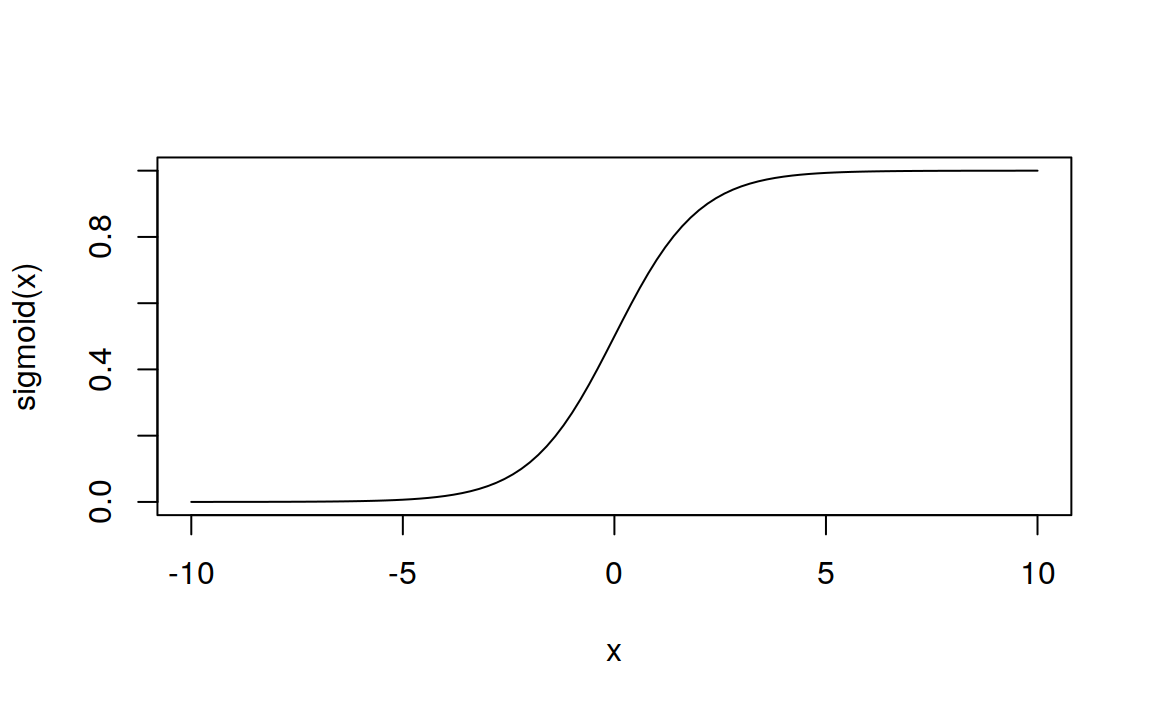
\includegraphics[width=0.7\linewidth]{regression_138-advertising_files/figure-latex/unnamed-chunk-7-1} \end{center}

\begin{Shaded}
\begin{Highlighting}[]
\NormalTok{tv_model}
\CommentTok{#> }
\CommentTok{#> Call:}
\CommentTok{#> lm(formula = sales ~ TV, data = advertising)}
\CommentTok{#> }
\CommentTok{#> Coefficients:}
\CommentTok{#> (Intercept)           TV  }
\CommentTok{#>      7.0326       0.0475}
\end{Highlighting}
\end{Shaded}

\begin{Shaded}
\begin{Highlighting}[]
\NormalTok{tv.lm <-}\StringTok{ }\KeywordTok{lm}\NormalTok{(sales }\OperatorTok{~}\StringTok{ }\KeywordTok{poly}\NormalTok{(sales, TV, }\DataTypeTok{degree=}\DecValTok{2}\NormalTok{), }\DataTypeTok{data =}\NormalTok{ advertising)}
\CommentTok{# contour(tv.lm, sales ~ TV)}
\end{Highlighting}
\end{Shaded}

\begin{Shaded}
\begin{Highlighting}[]
\KeywordTok{library}\NormalTok{(rsm)}
\NormalTok{mpg.lm <-}\StringTok{ }\KeywordTok{lm}\NormalTok{(mpg }\OperatorTok{~}\StringTok{ }\KeywordTok{poly}\NormalTok{(hp, disp, }\DataTypeTok{degree =} \DecValTok{3}\NormalTok{), }\DataTypeTok{data =}\NormalTok{ mtcars)}
\KeywordTok{contour}\NormalTok{(mpg.lm, hp }\OperatorTok{~}\StringTok{ }\NormalTok{disp)}
\end{Highlighting}
\end{Shaded}

\begin{center}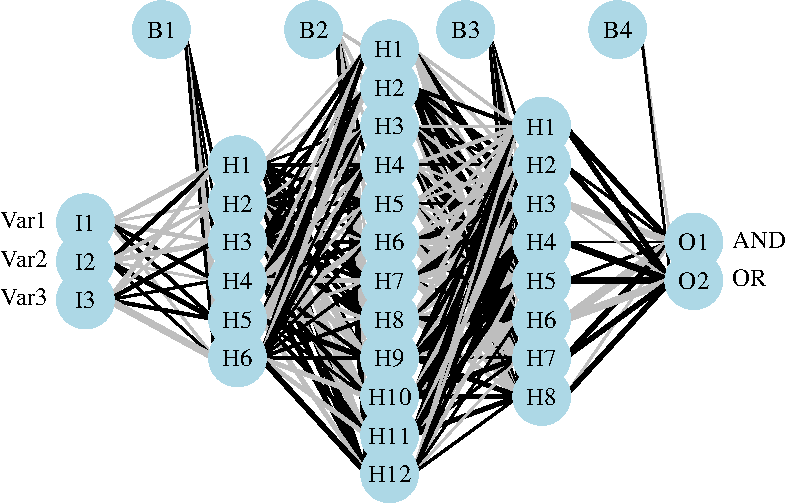
\includegraphics[width=0.7\linewidth]{regression_138-advertising_files/figure-latex/unnamed-chunk-10-1} \end{center}

\begin{Shaded}
\begin{Highlighting}[]
\NormalTok{x <-}\StringTok{ }\DecValTok{-6}\OperatorTok{:}\DecValTok{16}
\NormalTok{op <-}\StringTok{ }\KeywordTok{par}\NormalTok{(}\DataTypeTok{mfrow =} \KeywordTok{c}\NormalTok{(}\DecValTok{2}\NormalTok{, }\DecValTok{2}\NormalTok{))}
\KeywordTok{contour}\NormalTok{(}\KeywordTok{outer}\NormalTok{(x, x), }\DataTypeTok{method =} \StringTok{"flattest"}\NormalTok{, }\DataTypeTok{vfont =} \KeywordTok{c}\NormalTok{(}\StringTok{"sans serif"}\NormalTok{, }\StringTok{"plain"}\NormalTok{))}
\end{Highlighting}
\end{Shaded}

\begin{center}\includegraphics[width=0.7\linewidth]{regression_138-advertising_files/figure-latex/unnamed-chunk-11-1} \end{center}

\hypertarget{regression-3b.-rates-dataset}{%
\chapter{\texorpdfstring{Regression 3b. \texttt{Rates} dataset}{Regression 3b. Rates dataset}}\label{regression-3b.-rates-dataset}}

\hypertarget{introduction-1}{%
\section{Introduction}\label{introduction-1}}

\begin{quote}
line 29 does not plot
\end{quote}

\textbf{Source:} \url{https://www.matthewrenze.com/workshops/practical-machine-learning-with-r/lab-3b-regression.html}

\begin{Shaded}
\begin{Highlighting}[]
\KeywordTok{library}\NormalTok{(readr)}

\NormalTok{policies <-}\StringTok{ }\KeywordTok{read_csv}\NormalTok{(}\KeywordTok{file.path}\NormalTok{(data_raw_dir, }\StringTok{"Rates.csv"}\NormalTok{))}
\CommentTok{#> Parsed with column specification:}
\CommentTok{#> cols(}
\CommentTok{#>   Gender = col_character(),}
\CommentTok{#>   State = col_character(),}
\CommentTok{#>   State.Rate = col_double(),}
\CommentTok{#>   Height = col_double(),}
\CommentTok{#>   Weight = col_double(),}
\CommentTok{#>   BMI = col_double(),}
\CommentTok{#>   Age = col_double(),}
\CommentTok{#>   Rate = col_double()}
\CommentTok{#> )}
\NormalTok{policies}
\CommentTok{#> # A tibble: 1,942 x 8}
\CommentTok{#>   Gender State State.Rate Height Weight   BMI   Age   Rate}
\CommentTok{#>   <chr>  <chr>      <dbl>  <dbl>  <dbl> <dbl> <dbl>  <dbl>}
\CommentTok{#> 1 Male   MA        0.100     184   67.8  20.0    77 0.332 }
\CommentTok{#> 2 Male   VA        0.142     163   89.4  33.6    82 0.869 }
\CommentTok{#> 3 Male   NY        0.0908    170   81.2  28.1    31 0.01  }
\CommentTok{#> 4 Male   TN        0.120     175   99.7  32.6    39 0.0215}
\CommentTok{#> 5 Male   FL        0.110     184   72.1  21.3    68 0.150 }
\CommentTok{#> 6 Male   WA        0.163     166   98.4  35.7    64 0.211 }
\CommentTok{#> # ... with 1,936 more rows}
\end{Highlighting}
\end{Shaded}

\begin{Shaded}
\begin{Highlighting}[]
\KeywordTok{summary}\NormalTok{(policies)}
\CommentTok{#>     Gender             State             State.Rate        Height   }
\CommentTok{#>  Length:1942        Length:1942        Min.   :0.001   Min.   :150  }
\CommentTok{#>  Class :character   Class :character   1st Qu.:0.110   1st Qu.:162  }
\CommentTok{#>  Mode  :character   Mode  :character   Median :0.128   Median :170  }
\CommentTok{#>                                        Mean   :0.138   Mean   :170  }
\CommentTok{#>                                        3rd Qu.:0.144   3rd Qu.:176  }
\CommentTok{#>                                        Max.   :0.318   Max.   :190  }
\CommentTok{#>      Weight           BMI            Age            Rate      }
\CommentTok{#>  Min.   : 44.1   Min.   :16.0   Min.   :18.0   Min.   :0.001  }
\CommentTok{#>  1st Qu.: 68.6   1st Qu.:23.7   1st Qu.:34.0   1st Qu.:0.015  }
\CommentTok{#>  Median : 81.3   Median :28.1   Median :51.0   Median :0.046  }
\CommentTok{#>  Mean   : 81.2   Mean   :28.3   Mean   :50.8   Mean   :0.138  }
\CommentTok{#>  3rd Qu.: 93.8   3rd Qu.:32.5   3rd Qu.:68.0   3rd Qu.:0.173  }
\CommentTok{#>  Max.   :116.5   Max.   :46.8   Max.   :84.0   Max.   :0.999}
\end{Highlighting}
\end{Shaded}

\begin{Shaded}
\begin{Highlighting}[]
\KeywordTok{library}\NormalTok{(RColorBrewer)}
\NormalTok{palette <-}\StringTok{ }\KeywordTok{brewer.pal}\NormalTok{(}\DecValTok{9}\NormalTok{, }\StringTok{"Reds"}\NormalTok{)}
\end{Highlighting}
\end{Shaded}

\begin{Shaded}
\begin{Highlighting}[]
\CommentTok{# plot(}
\CommentTok{#   x = policies,}
\CommentTok{#   col = palette[cut(x = policies$Rate, breaks = 9)]}
\CommentTok{#   )}
\end{Highlighting}
\end{Shaded}

\begin{Shaded}
\begin{Highlighting}[]
\KeywordTok{library}\NormalTok{(corrgram)}
\CommentTok{#> Registered S3 methods overwritten by 'ggplot2':}
\CommentTok{#>   method         from }
\CommentTok{#>   [.quosures     rlang}
\CommentTok{#>   c.quosures     rlang}
\CommentTok{#>   print.quosures rlang}
\CommentTok{#> Registered S3 method overwritten by 'seriation':}
\CommentTok{#>   method         from }
\CommentTok{#>   reorder.hclust gclus}

\KeywordTok{corrgram}\NormalTok{(policies)}
\end{Highlighting}
\end{Shaded}

\begin{center}\includegraphics[width=0.7\linewidth]{regression_141.2-3b_files/figure-latex/unnamed-chunk-6-1} \end{center}

\begin{Shaded}
\begin{Highlighting}[]
\KeywordTok{cor}\NormalTok{(policies[}\DecValTok{3}\OperatorTok{:}\DecValTok{8}\NormalTok{])}
\CommentTok{#>            State.Rate  Height  Weight     BMI     Age    Rate}
\CommentTok{#> State.Rate    1.00000 -0.0165 0.00923  0.0192  0.1123  0.2269}
\CommentTok{#> Height       -0.01652  1.0000 0.23809 -0.3170 -0.1648 -0.1286}
\CommentTok{#> Weight        0.00923  0.2381 1.00000  0.8396  0.0117  0.0609}
\CommentTok{#> BMI           0.01924 -0.3170 0.83963  1.0000  0.1023  0.1405}
\CommentTok{#> Age           0.11235 -0.1648 0.01168  0.1023  1.0000  0.7801}
\CommentTok{#> Rate          0.22685 -0.1286 0.06094  0.1405  0.7801  1.0000}
\end{Highlighting}
\end{Shaded}

\begin{Shaded}
\begin{Highlighting}[]
\KeywordTok{cor}\NormalTok{(}
  \DataTypeTok{x =}\NormalTok{ policies}\OperatorTok{$}\NormalTok{Age, }
  \DataTypeTok{y =}\NormalTok{ policies}\OperatorTok{$}\NormalTok{Rate)}
\CommentTok{#> [1] 0.78}
\end{Highlighting}
\end{Shaded}

\begin{Shaded}
\begin{Highlighting}[]
\KeywordTok{plot}\NormalTok{(}
  \DataTypeTok{x =}\NormalTok{ policies}\OperatorTok{$}\NormalTok{Age, }
  \DataTypeTok{y =}\NormalTok{ policies}\OperatorTok{$}\NormalTok{Rate)}
\end{Highlighting}
\end{Shaded}

\begin{center}\includegraphics[width=0.7\linewidth]{regression_141.2-3b_files/figure-latex/unnamed-chunk-9-1} \end{center}

\hypertarget{split-the-data-into-test-and-training-sets}{%
\section{Split the Data into Test and Training Sets}\label{split-the-data-into-test-and-training-sets}}

\begin{Shaded}
\begin{Highlighting}[]
\KeywordTok{set.seed}\NormalTok{(}\DecValTok{42}\NormalTok{)}
\end{Highlighting}
\end{Shaded}

\begin{Shaded}
\begin{Highlighting}[]
\KeywordTok{library}\NormalTok{(caret)}
\CommentTok{#> Loading required package: lattice}
\CommentTok{#> }
\CommentTok{#> Attaching package: 'lattice'}
\CommentTok{#> The following object is masked from 'package:corrgram':}
\CommentTok{#> }
\CommentTok{#>     panel.fill}
\CommentTok{#> Loading required package: ggplot2}

\NormalTok{indexes <-}\StringTok{ }\KeywordTok{createDataPartition}\NormalTok{(}
  \DataTypeTok{y =}\NormalTok{ policies}\OperatorTok{$}\NormalTok{Rate,}
  \DataTypeTok{p =} \FloatTok{0.80}\NormalTok{,}
  \DataTypeTok{list =} \OtherTok{FALSE}\NormalTok{)}

\NormalTok{train <-}\StringTok{ }\NormalTok{policies[indexes, ]}
\NormalTok{test <-}\StringTok{ }\NormalTok{policies[}\OperatorTok{-}\NormalTok{indexes, ]}
\end{Highlighting}
\end{Shaded}

\begin{Shaded}
\begin{Highlighting}[]
\KeywordTok{print}\NormalTok{(}\KeywordTok{nrow}\NormalTok{(train))}
\CommentTok{#> [1] 1555}
\KeywordTok{print}\NormalTok{(}\KeywordTok{nrow}\NormalTok{(test))}
\CommentTok{#> [1] 387}
\end{Highlighting}
\end{Shaded}

\hypertarget{predict-with-simple-linear-regression}{%
\section{Predict with Simple Linear Regression}\label{predict-with-simple-linear-regression}}

\begin{Shaded}
\begin{Highlighting}[]
\NormalTok{simpleModel <-}\StringTok{ }\KeywordTok{lm}\NormalTok{(}
  \DataTypeTok{formula =}\NormalTok{ Rate }\OperatorTok{~}\StringTok{ }\NormalTok{Age,}
  \DataTypeTok{data =}\NormalTok{ train)}
\end{Highlighting}
\end{Shaded}

\begin{Shaded}
\begin{Highlighting}[]
\KeywordTok{plot}\NormalTok{(}
  \DataTypeTok{x =}\NormalTok{ policies}\OperatorTok{$}\NormalTok{Age, }
  \DataTypeTok{y =}\NormalTok{ policies}\OperatorTok{$}\NormalTok{Rate)}
  
\KeywordTok{lines}\NormalTok{(}
  \DataTypeTok{x =}\NormalTok{ train}\OperatorTok{$}\NormalTok{Age,}
  \DataTypeTok{y =}\NormalTok{ simpleModel}\OperatorTok{$}\NormalTok{fitted, }
  \DataTypeTok{col =} \StringTok{"red"}\NormalTok{,}
  \DataTypeTok{lwd =} \DecValTok{3}\NormalTok{)}
\end{Highlighting}
\end{Shaded}

\begin{center}\includegraphics[width=0.7\linewidth]{regression_141.2-3b_files/figure-latex/unnamed-chunk-14-1} \end{center}

\begin{Shaded}
\begin{Highlighting}[]
\KeywordTok{summary}\NormalTok{(simpleModel)}
\CommentTok{#> }
\CommentTok{#> Call:}
\CommentTok{#> lm(formula = Rate ~ Age, data = train)}
\CommentTok{#> }
\CommentTok{#> Residuals:}
\CommentTok{#>     Min      1Q  Median      3Q     Max }
\CommentTok{#> -0.1799 -0.0881 -0.0208  0.0617  0.6300 }
\CommentTok{#> }
\CommentTok{#> Coefficients:}
\CommentTok{#>              Estimate Std. Error t value Pr(>|t|)    }
\CommentTok{#> (Intercept) -0.265244   0.008780   -30.2   <2e-16 ***}
\CommentTok{#> Age          0.007928   0.000161    49.3   <2e-16 ***}
\CommentTok{#> ---}
\CommentTok{#> Signif. codes:  0 '***' 0.001 '**' 0.01 '*' 0.05 '.' 0.1 ' ' 1}
\CommentTok{#> }
\CommentTok{#> Residual standard error: 0.123 on 1553 degrees of freedom}
\CommentTok{#> Multiple R-squared:  0.61,   Adjusted R-squared:  0.609 }
\CommentTok{#> F-statistic: 2.43e+03 on 1 and 1553 DF,  p-value: <2e-16}
\end{Highlighting}
\end{Shaded}

\begin{Shaded}
\begin{Highlighting}[]
\NormalTok{simplePredictions <-}\StringTok{ }\KeywordTok{predict}\NormalTok{(}
  \DataTypeTok{object =}\NormalTok{ simpleModel,}
  \DataTypeTok{newdata =}\NormalTok{ test)}
\end{Highlighting}
\end{Shaded}

\begin{Shaded}
\begin{Highlighting}[]
\KeywordTok{plot}\NormalTok{(}
  \DataTypeTok{x =}\NormalTok{ policies}\OperatorTok{$}\NormalTok{Age, }
  \DataTypeTok{y =}\NormalTok{ policies}\OperatorTok{$}\NormalTok{Rate)}


\KeywordTok{points}\NormalTok{(}
  \DataTypeTok{x =}\NormalTok{ test}\OperatorTok{$}\NormalTok{Age,}
  \DataTypeTok{y =}\NormalTok{ simplePredictions,}
  \DataTypeTok{col =} \StringTok{"blue"}\NormalTok{,}
  \DataTypeTok{pch =} \DecValTok{4}\NormalTok{,}
  \DataTypeTok{lwd =} \DecValTok{2}\NormalTok{)}
\end{Highlighting}
\end{Shaded}

\begin{center}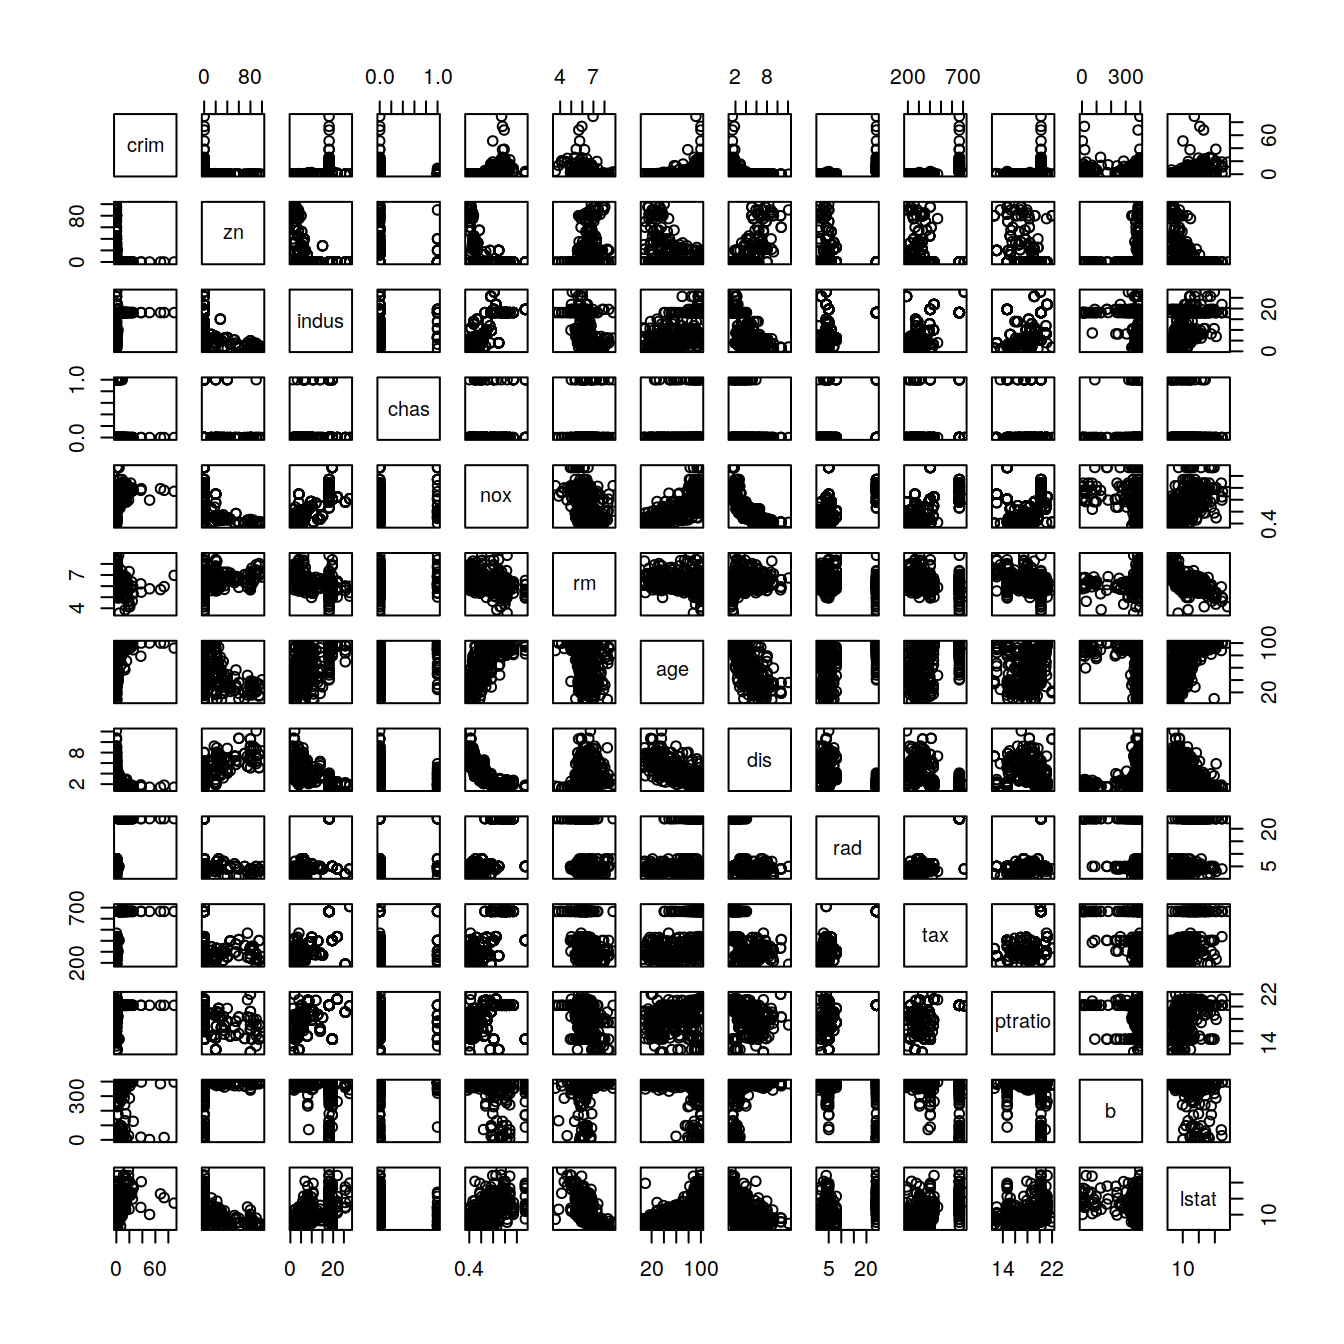
\includegraphics[width=0.7\linewidth]{regression_141.2-3b_files/figure-latex/unnamed-chunk-17-1} \end{center}

\begin{Shaded}
\begin{Highlighting}[]
\NormalTok{simpleRMSE <-}\StringTok{ }\KeywordTok{sqrt}\NormalTok{(}\KeywordTok{mean}\NormalTok{((test}\OperatorTok{$}\NormalTok{Rate }\OperatorTok{-}\StringTok{ }\NormalTok{simplePredictions)}\OperatorTok{^}\DecValTok{2}\NormalTok{))}
\KeywordTok{print}\NormalTok{(simpleRMSE)}
\CommentTok{#> [1] 0.119}
\end{Highlighting}
\end{Shaded}

\hypertarget{predict-with-multiple-linear-regression}{%
\section{Predict with Multiple Linear Regression}\label{predict-with-multiple-linear-regression}}

\begin{Shaded}
\begin{Highlighting}[]
\NormalTok{multipleModel <-}\StringTok{ }\KeywordTok{lm}\NormalTok{(}
  \DataTypeTok{formula =}\NormalTok{ Rate }\OperatorTok{~}\StringTok{ }\NormalTok{Age }\OperatorTok{+}\StringTok{ }\NormalTok{Gender }\OperatorTok{+}\StringTok{ }\NormalTok{State.Rate }\OperatorTok{+}\StringTok{ }\NormalTok{BMI,}
  \DataTypeTok{data =}\NormalTok{ train)}
\end{Highlighting}
\end{Shaded}

\begin{Shaded}
\begin{Highlighting}[]
\KeywordTok{summary}\NormalTok{(multipleModel)}
\CommentTok{#> }
\CommentTok{#> Call:}
\CommentTok{#> lm(formula = Rate ~ Age + Gender + State.Rate + BMI, data = train)}
\CommentTok{#> }
\CommentTok{#> Residuals:}
\CommentTok{#>     Min      1Q  Median      3Q     Max }
\CommentTok{#> -0.2255 -0.0865 -0.0292  0.0590  0.6053 }
\CommentTok{#> }
\CommentTok{#> Coefficients:}
\CommentTok{#>              Estimate Std. Error t value Pr(>|t|)    }
\CommentTok{#> (Intercept) -0.428141   0.018742  -22.84  < 2e-16 ***}
\CommentTok{#> Age          0.007703   0.000156   49.28  < 2e-16 ***}
\CommentTok{#> GenderMale   0.030350   0.006001    5.06  4.8e-07 ***}
\CommentTok{#> State.Rate   0.613139   0.068330    8.97  < 2e-16 ***}
\CommentTok{#> BMI          0.002634   0.000518    5.09  4.1e-07 ***}
\CommentTok{#> ---}
\CommentTok{#> Signif. codes:  0 '***' 0.001 '**' 0.01 '*' 0.05 '.' 0.1 ' ' 1}
\CommentTok{#> }
\CommentTok{#> Residual standard error: 0.118 on 1550 degrees of freedom}
\CommentTok{#> Multiple R-squared:  0.64,   Adjusted R-squared:  0.639 }
\CommentTok{#> F-statistic:  688 on 4 and 1550 DF,  p-value: <2e-16}
\end{Highlighting}
\end{Shaded}

\begin{Shaded}
\begin{Highlighting}[]
\NormalTok{multiplePredictions <-}\StringTok{ }\KeywordTok{predict}\NormalTok{(}
  \DataTypeTok{object =}\NormalTok{ multipleModel,}
  \DataTypeTok{newdata =}\NormalTok{ test)}
\end{Highlighting}
\end{Shaded}

\begin{Shaded}
\begin{Highlighting}[]
\KeywordTok{plot}\NormalTok{(}
  \DataTypeTok{x =}\NormalTok{ policies}\OperatorTok{$}\NormalTok{Age, }
  \DataTypeTok{y =}\NormalTok{ policies}\OperatorTok{$}\NormalTok{Rate)}

\KeywordTok{points}\NormalTok{(}
  \DataTypeTok{x =}\NormalTok{ test}\OperatorTok{$}\NormalTok{Age,}
  \DataTypeTok{y =}\NormalTok{ multiplePredictions,}
  \DataTypeTok{col =} \StringTok{"blue"}\NormalTok{,}
  \DataTypeTok{pch =} \DecValTok{4}\NormalTok{,}
  \DataTypeTok{lwd =} \DecValTok{2}\NormalTok{)}
\end{Highlighting}
\end{Shaded}

\begin{center}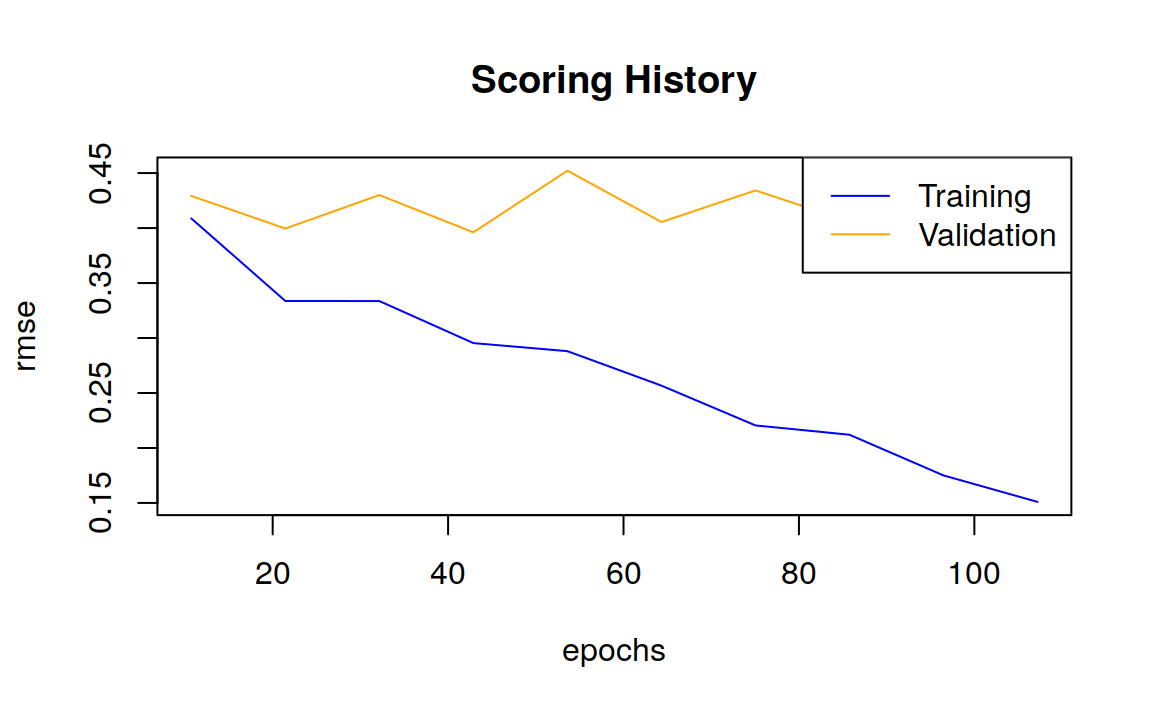
\includegraphics[width=0.7\linewidth]{regression_141.2-3b_files/figure-latex/unnamed-chunk-22-1} \end{center}

\begin{Shaded}
\begin{Highlighting}[]
\NormalTok{multipleRMSE <-}\StringTok{ }\KeywordTok{sqrt}\NormalTok{(}\KeywordTok{mean}\NormalTok{((test}\OperatorTok{$}\NormalTok{Rate }\OperatorTok{-}\StringTok{ }\NormalTok{multiplePredictions)}\OperatorTok{^}\DecValTok{2}\NormalTok{))}
\KeywordTok{print}\NormalTok{(multipleRMSE)}
\CommentTok{#> [1] 0.114}
\end{Highlighting}
\end{Shaded}

\hypertarget{predict-with-neural-network-regression}{%
\section{Predict with Neural Network Regression}\label{predict-with-neural-network-regression}}

\begin{Shaded}
\begin{Highlighting}[]
\NormalTok{normalize <-}\StringTok{ }\ControlFlowTok{function}\NormalTok{(x) \{}
\NormalTok{  (x }\OperatorTok{-}\StringTok{ }\KeywordTok{min}\NormalTok{(x)) }\OperatorTok{/}\StringTok{ }\NormalTok{(}\KeywordTok{max}\NormalTok{(x) }\OperatorTok{-}\StringTok{ }\KeywordTok{min}\NormalTok{(x)) }\OperatorTok{-}\StringTok{ }\FloatTok{0.5}
\NormalTok{\}}
\end{Highlighting}
\end{Shaded}

\begin{Shaded}
\begin{Highlighting}[]
\NormalTok{denormalize <-}\StringTok{ }\ControlFlowTok{function}\NormalTok{(x, y) \{}
\NormalTok{  ((x }\OperatorTok{+}\StringTok{ }\FloatTok{0.5}\NormalTok{) }\OperatorTok{*}\StringTok{ }\NormalTok{(}\KeywordTok{max}\NormalTok{(y) }\OperatorTok{-}\StringTok{ }\KeywordTok{min}\NormalTok{(y))) }\OperatorTok{+}\StringTok{ }\KeywordTok{min}\NormalTok{(y)}
\NormalTok{\}}
\end{Highlighting}
\end{Shaded}

\begin{Shaded}
\begin{Highlighting}[]
\NormalTok{scaledPolicies <-}\StringTok{ }\KeywordTok{data.frame}\NormalTok{(}
  \DataTypeTok{Gender =}\NormalTok{ policies}\OperatorTok{$}\NormalTok{Gender,}
  \DataTypeTok{State.Rate =} \KeywordTok{normalize}\NormalTok{(policies}\OperatorTok{$}\NormalTok{State.Rate),}
  \DataTypeTok{BMI =} \KeywordTok{normalize}\NormalTok{(policies}\OperatorTok{$}\NormalTok{BMI),}
  \DataTypeTok{Age =} \KeywordTok{normalize}\NormalTok{(policies}\OperatorTok{$}\NormalTok{Age),}
  \DataTypeTok{Rate =} \KeywordTok{normalize}\NormalTok{(policies}\OperatorTok{$}\NormalTok{Rate))}
\end{Highlighting}
\end{Shaded}

\begin{Shaded}
\begin{Highlighting}[]
\NormalTok{scaledTrain <-}\StringTok{ }\NormalTok{scaledPolicies[indexes, ]}
\NormalTok{scaledTest <-}\StringTok{ }\NormalTok{scaledPolicies[}\OperatorTok{-}\NormalTok{indexes, ]}
\end{Highlighting}
\end{Shaded}

\begin{Shaded}
\begin{Highlighting}[]
\KeywordTok{library}\NormalTok{(nnet)}

\NormalTok{neuralRegressor <-}\StringTok{ }\KeywordTok{nnet}\NormalTok{(}
  \DataTypeTok{formula =}\NormalTok{ Rate }\OperatorTok{~}\StringTok{ }\NormalTok{.,}
  \DataTypeTok{data =}\NormalTok{ scaledTrain,}
  \DataTypeTok{linout =} \OtherTok{TRUE}\NormalTok{,}
  \DataTypeTok{size =} \DecValTok{5}\NormalTok{,}
  \DataTypeTok{decay =} \FloatTok{0.0001}\NormalTok{,}
  \DataTypeTok{maxit =} \DecValTok{1000}\NormalTok{)}
\CommentTok{#> # weights:  31}
\CommentTok{#> initial  value 548.090539 }
\CommentTok{#> iter  10 value 10.610284}
\CommentTok{#> iter  20 value 3.927378}
\CommentTok{#> iter  30 value 3.735266}
\CommentTok{#> iter  40 value 3.513899}
\CommentTok{#> iter  50 value 3.073390}
\CommentTok{#> iter  60 value 2.547202}
\CommentTok{#> iter  70 value 2.296126}
\CommentTok{#> iter  80 value 2.166120}
\CommentTok{#> iter  90 value 2.106996}
\CommentTok{#> iter 100 value 2.092654}
\CommentTok{#> iter 110 value 2.058596}
\CommentTok{#> iter 120 value 2.039404}
\CommentTok{#> iter 130 value 2.023721}
\CommentTok{#> iter 140 value 2.018781}
\CommentTok{#> iter 150 value 2.006931}
\CommentTok{#> iter 160 value 1.999122}
\CommentTok{#> iter 170 value 1.993920}
\CommentTok{#> iter 180 value 1.990678}
\CommentTok{#> iter 190 value 1.989269}
\CommentTok{#> iter 200 value 1.988846}
\CommentTok{#> iter 210 value 1.988042}
\CommentTok{#> iter 220 value 1.987739}
\CommentTok{#> iter 230 value 1.987678}
\CommentTok{#> iter 240 value 1.987598}
\CommentTok{#> iter 250 value 1.987574}
\CommentTok{#> iter 260 value 1.987549}
\CommentTok{#> iter 270 value 1.987536}
\CommentTok{#> iter 280 value 1.987529}
\CommentTok{#> final  value 1.987526 }
\CommentTok{#> converged}
\end{Highlighting}
\end{Shaded}

\begin{Shaded}
\begin{Highlighting}[]
\NormalTok{scaledPredictions <-}\StringTok{ }\KeywordTok{predict}\NormalTok{(}
  \DataTypeTok{object =}\NormalTok{ neuralRegressor, }
  \DataTypeTok{newdata =}\NormalTok{ scaledTest)}
\end{Highlighting}
\end{Shaded}

\begin{Shaded}
\begin{Highlighting}[]
\NormalTok{neuralPredictions <-}\StringTok{ }\KeywordTok{denormalize}\NormalTok{(}
  \DataTypeTok{x =}\NormalTok{ scaledPredictions, }
  \DataTypeTok{y =}\NormalTok{ policies}\OperatorTok{$}\NormalTok{Rate)}
\end{Highlighting}
\end{Shaded}

\begin{Shaded}
\begin{Highlighting}[]
\KeywordTok{plot}\NormalTok{(}
  \DataTypeTok{x =}\NormalTok{ train}\OperatorTok{$}\NormalTok{Age, }
  \DataTypeTok{y =}\NormalTok{ train}\OperatorTok{$}\NormalTok{Rate)}

\KeywordTok{points}\NormalTok{(}
  \DataTypeTok{x =}\NormalTok{ test}\OperatorTok{$}\NormalTok{Age,}
  \DataTypeTok{y =}\NormalTok{ neuralPredictions,}
  \DataTypeTok{col =} \StringTok{"blue"}\NormalTok{,}
  \DataTypeTok{pch =} \DecValTok{4}\NormalTok{,}
  \DataTypeTok{lwd =} \DecValTok{2}\NormalTok{)}
\end{Highlighting}
\end{Shaded}

\begin{center}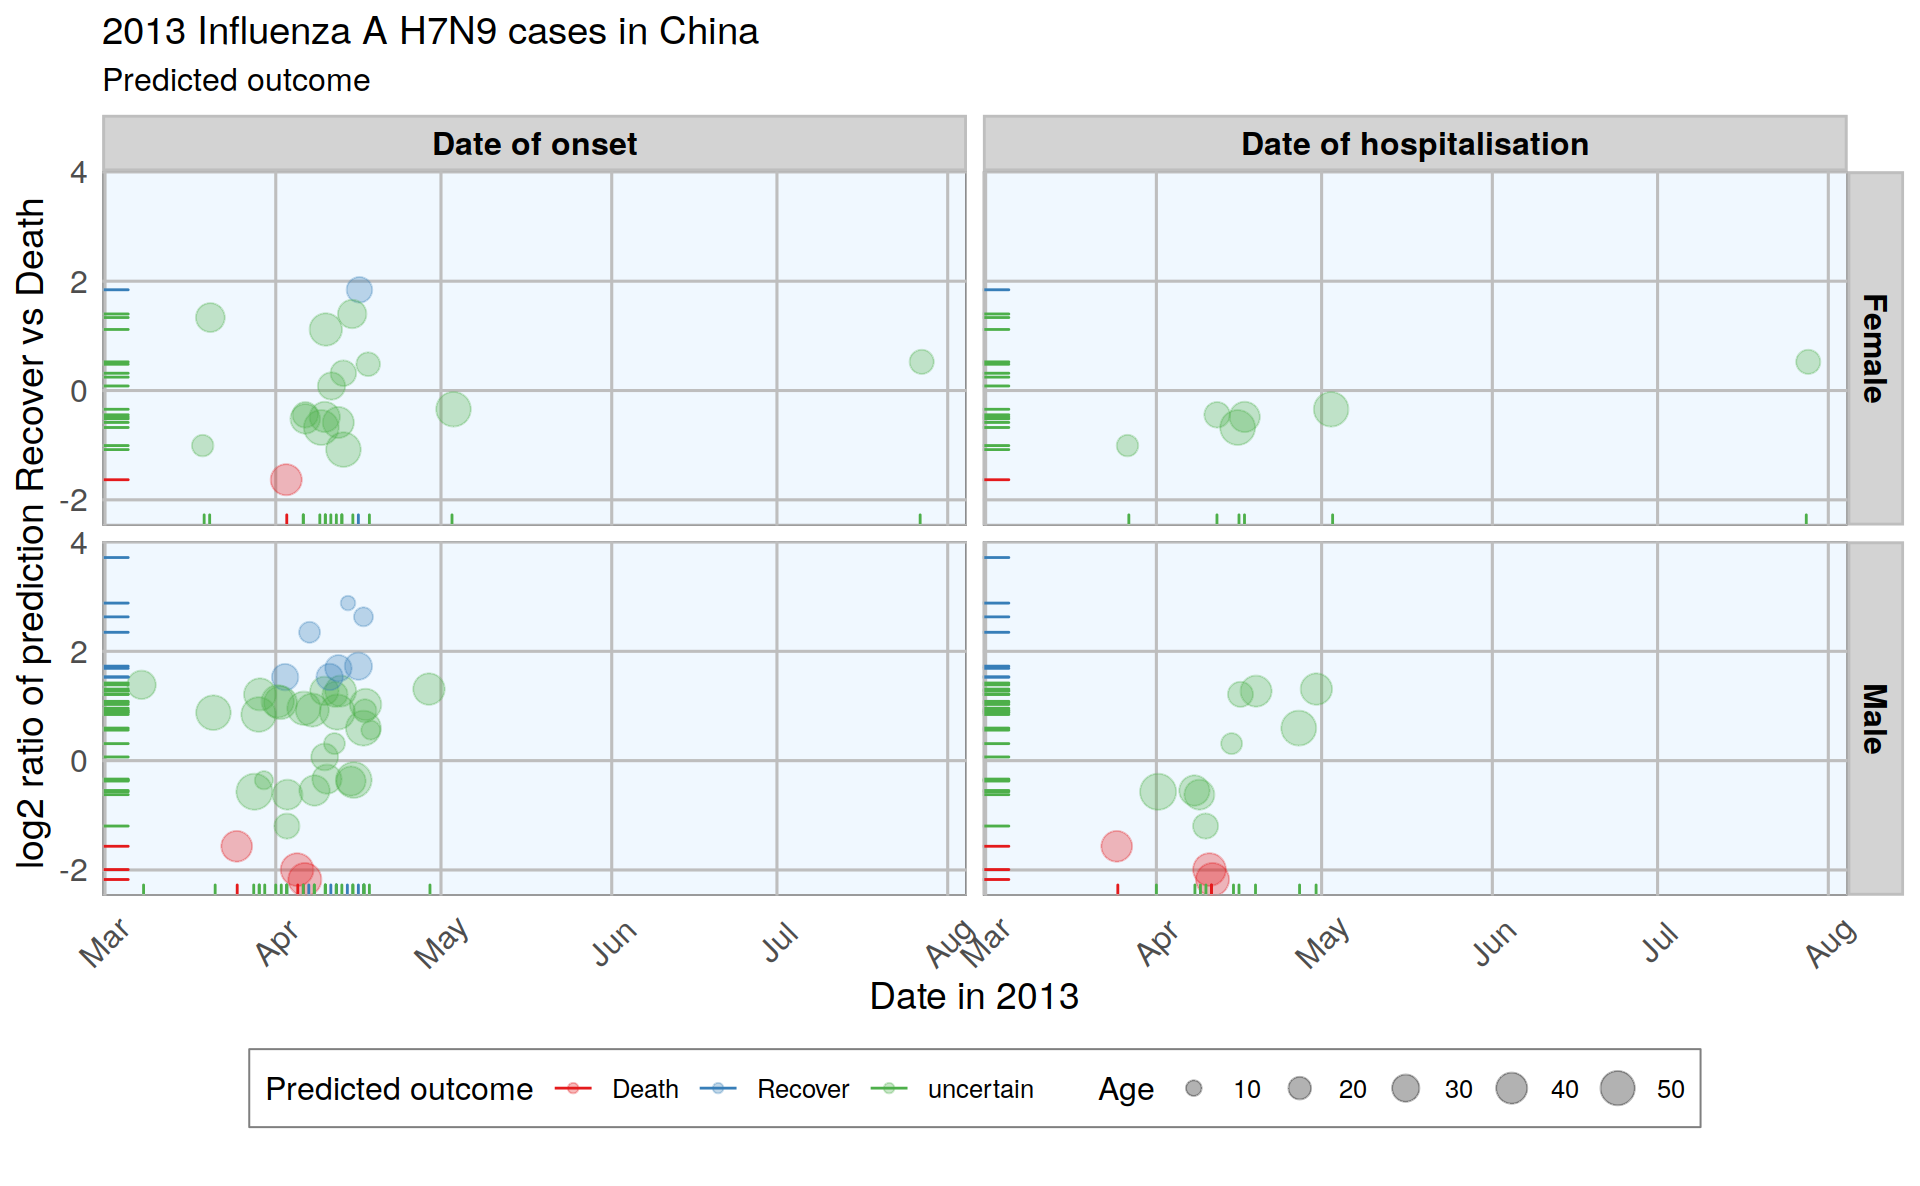
\includegraphics[width=0.7\linewidth]{regression_141.2-3b_files/figure-latex/unnamed-chunk-31-1} \end{center}

\begin{Shaded}
\begin{Highlighting}[]
\KeywordTok{library}\NormalTok{(NeuralNetTools)}

\KeywordTok{plotnet}\NormalTok{(neuralRegressor)}
\end{Highlighting}
\end{Shaded}

\begin{center}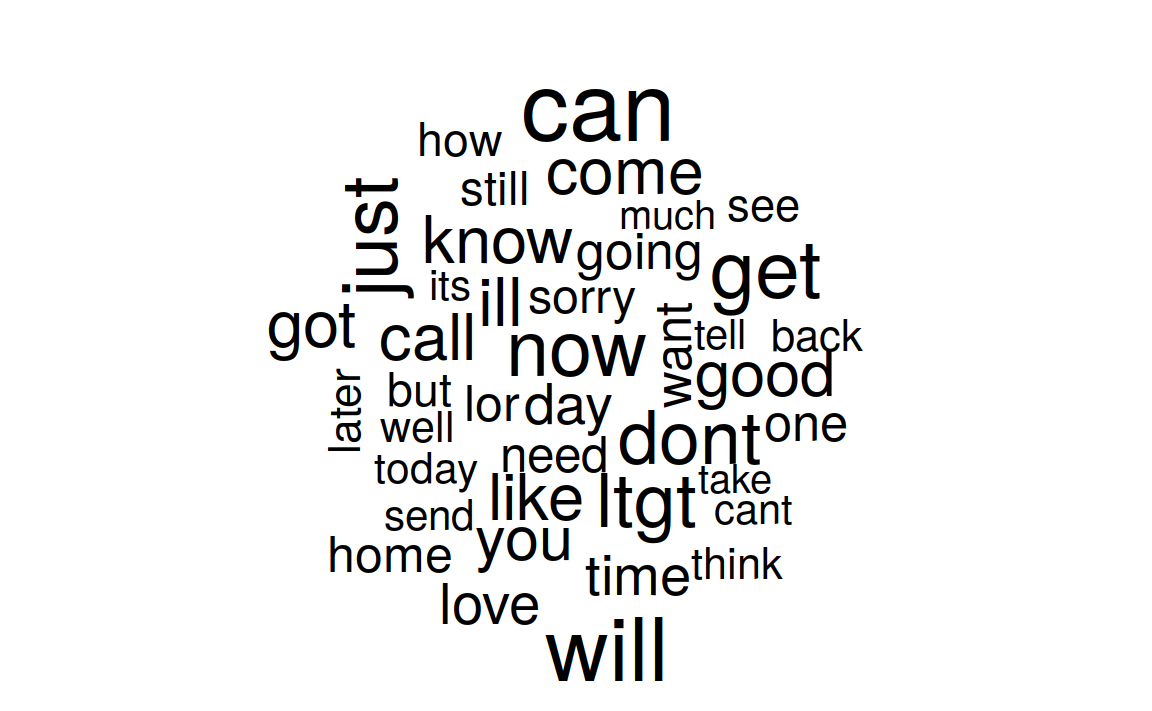
\includegraphics[width=0.7\linewidth]{regression_141.2-3b_files/figure-latex/unnamed-chunk-32-1} \end{center}

\begin{Shaded}
\begin{Highlighting}[]
\NormalTok{neuralRMSE <-}\StringTok{ }\KeywordTok{sqrt}\NormalTok{(}\KeywordTok{mean}\NormalTok{((test}\OperatorTok{$}\NormalTok{Rate }\OperatorTok{-}\StringTok{ }\NormalTok{neuralPredictions)}\OperatorTok{^}\DecValTok{2}\NormalTok{))}
\KeywordTok{print}\NormalTok{(neuralRMSE)}
\CommentTok{#> [1] 0.0368}
\end{Highlighting}
\end{Shaded}

\hypertarget{evaluate-the-regression-models}{%
\section{Evaluate the Regression Models}\label{evaluate-the-regression-models}}

\begin{Shaded}
\begin{Highlighting}[]
\KeywordTok{print}\NormalTok{(simpleRMSE)}
\CommentTok{#> [1] 0.119}
\KeywordTok{print}\NormalTok{(multipleRMSE)}
\CommentTok{#> [1] 0.114}
\KeywordTok{print}\NormalTok{(neuralRMSE)}
\CommentTok{#> [1] 0.0368}
\end{Highlighting}
\end{Shaded}

\hypertarget{regression-with-ann---yacht-hydrodynamics}{%
\chapter{Regression with ANN - Yacht Hydrodynamics}\label{regression-with-ann---yacht-hydrodynamics}}

\hypertarget{introduction-2}{%
\section{Introduction}\label{introduction-2}}

Regression ANNs predict an output variable as a function of the inputs. The input features (independent variables) can be categorical or numeric types, however, for regression ANNs, we require a numeric dependent variable. If the output variable is a categorical variable (or binary) the ANN will function as a classifier (see next tutorial).

Source: \url{http://uc-r.github.io/ann_regression}

In this tutorial we introduce a neural network used for numeric predictions and cover:

\begin{itemize}
\tightlist
\item
  Replication requirements: What you'll need to reproduce the analysis in this tutorial.
\item
  Data Preparation: Preparing our data.
\item
  1st Regression ANN: Constructing a 1-hidden layer ANN with 1 neuron.
\item
  Regression Hyperparameters: Tuning the model.
\item
  Wrapping Up: Final comments and some exercises to test your skills.
\end{itemize}

\hypertarget{replication-requirements}{%
\section{Replication Requirements}\label{replication-requirements}}

We require the following packages for the analysis.

\begin{Shaded}
\begin{Highlighting}[]
\KeywordTok{library}\NormalTok{(tidyverse)}
\CommentTok{#> Registered S3 methods overwritten by 'ggplot2':}
\CommentTok{#>   method         from }
\CommentTok{#>   [.quosures     rlang}
\CommentTok{#>   c.quosures     rlang}
\CommentTok{#>   print.quosures rlang}
\CommentTok{#> Registered S3 method overwritten by 'rvest':}
\CommentTok{#>   method            from}
\CommentTok{#>   read_xml.response xml2}
\CommentTok{#> -- Attaching packages -------------------------------------------- tidyverse 1.2.1 --}
\CommentTok{#> v ggplot2 3.1.1       v purrr   0.3.2  }
\CommentTok{#> v tibble  2.1.1       v dplyr   0.8.0.1}
\CommentTok{#> v tidyr   0.8.3       v stringr 1.4.0  }
\CommentTok{#> v readr   1.3.1       v forcats 0.4.0}
\CommentTok{#> -- Conflicts ----------------------------------------------- tidyverse_conflicts() --}
\CommentTok{#> x dplyr::filter() masks stats::filter()}
\CommentTok{#> x dplyr::lag()    masks stats::lag()}
\KeywordTok{library}\NormalTok{(neuralnet)}
\CommentTok{#> }
\CommentTok{#> Attaching package: 'neuralnet'}
\CommentTok{#> The following object is masked from 'package:dplyr':}
\CommentTok{#> }
\CommentTok{#>     compute}
\KeywordTok{library}\NormalTok{(GGally)}
\CommentTok{#> Registered S3 method overwritten by 'GGally':}
\CommentTok{#>   method from   }
\CommentTok{#>   +.gg   ggplot2}
\CommentTok{#> }
\CommentTok{#> Attaching package: 'GGally'}
\CommentTok{#> The following object is masked from 'package:dplyr':}
\CommentTok{#> }
\CommentTok{#>     nasa}
\end{Highlighting}
\end{Shaded}

\hypertarget{data-preparation}{%
\section{Data Preparation}\label{data-preparation}}

Our regression ANN will use the \textbf{Yacht Hydrodynamics} data set from UCI's Machine Learning Repository. The yacht data was provided by Dr.~Roberto Lopez email. This data set contains data contains results from 308 full-scale experiments performed at the Delft Ship Hydromechanics Laboratory where they test 22 different hull forms. Their experiment tested the effect of variations in the hull geometry and the ship's Froude number on the craft's residuary resistance per unit weight of displacement.

To begin we download the data from UCI.

\begin{Shaded}
\begin{Highlighting}[]
\NormalTok{url <-}\StringTok{ 'http://archive.ics.uci.edu/ml/machine-learning-databases/00243/yacht_hydrodynamics.data'}

\NormalTok{Yacht_Data <-}\StringTok{ }\KeywordTok{read_table}\NormalTok{(}\DataTypeTok{file =}\NormalTok{ url,}
                         \DataTypeTok{col_names =} \KeywordTok{c}\NormalTok{(}\StringTok{'LongPos_COB'}\NormalTok{, }\StringTok{'Prismatic_Coeff'}\NormalTok{,}
                                       \StringTok{'Len_Disp_Ratio'}\NormalTok{, }\StringTok{'Beam_Draut_Ratio'}\NormalTok{, }
                                       \StringTok{'Length_Beam_Ratio'}\NormalTok{,}\StringTok{'Froude_Num'}\NormalTok{, }
                                       \StringTok{'Residuary_Resist'}\NormalTok{)) }\OperatorTok
\StringTok{  }\KeywordTok{na.omit}\NormalTok{()}
\CommentTok{#> Parsed with column specification:}
\CommentTok{#> cols(}
\CommentTok{#>   LongPos_COB = col_double(),}
\CommentTok{#>   Prismatic_Coeff = col_double(),}
\CommentTok{#>   Len_Disp_Ratio = col_double(),}
\CommentTok{#>   Beam_Draut_Ratio = col_double(),}
\CommentTok{#>   Length_Beam_Ratio = col_double(),}
\CommentTok{#>   Froude_Num = col_double(),}
\CommentTok{#>   Residuary_Resist = col_double()}
\CommentTok{#> )}
\end{Highlighting}
\end{Shaded}

\begin{Shaded}
\begin{Highlighting}[]
\NormalTok{dplyr}\OperatorTok{::}\KeywordTok{glimpse}\NormalTok{(Yacht_Data)}
\CommentTok{#> Observations: 308}
\CommentTok{#> Variables: 7}
\CommentTok{#> $ LongPos_COB       <dbl> -2.3, -2.3, -2.3, -2.3, -2.3, -2.3, -2.3, -2...}
\CommentTok{#> $ Prismatic_Coeff   <dbl> 0.568, 0.568, 0.568, 0.568, 0.568, 0.568, 0....}
\CommentTok{#> $ Len_Disp_Ratio    <dbl> 4.78, 4.78, 4.78, 4.78, 4.78, 4.78, 4.78, 4....}
\CommentTok{#> $ Beam_Draut_Ratio  <dbl> 3.99, 3.99, 3.99, 3.99, 3.99, 3.99, 3.99, 3....}
\CommentTok{#> $ Length_Beam_Ratio <dbl> 3.17, 3.17, 3.17, 3.17, 3.17, 3.17, 3.17, 3....}
\CommentTok{#> $ Froude_Num        <dbl> 0.125, 0.150, 0.175, 0.200, 0.225, 0.250, 0....}
\CommentTok{#> $ Residuary_Resist  <dbl> 0.11, 0.27, 0.47, 0.78, 1.18, 1.82, 2.61, 3....}
\end{Highlighting}
\end{Shaded}

\begin{Shaded}
\begin{Highlighting}[]
\CommentTok{# save the dataset locally}
\KeywordTok{write.csv}\NormalTok{(Yacht_Data, }\DataTypeTok{file =} \KeywordTok{file.path}\NormalTok{(data_raw_dir, }\StringTok{"yach_data.csv"}\NormalTok{))}
\end{Highlighting}
\end{Shaded}

Prior to any data analysis lets take a look at the data set.

\begin{Shaded}
\begin{Highlighting}[]
\KeywordTok{ggpairs}\NormalTok{(Yacht_Data, }\DataTypeTok{title =} \StringTok{"Scatterplot Matrix of the Features of the Yacht Data Set"}\NormalTok{)}
\end{Highlighting}
\end{Shaded}

\begin{center}\includegraphics[width=0.7\linewidth]{regression_142-neural_network_yacht_files/figure-latex/unnamed-chunk-6-1} \end{center}

Here we see an excellent summary of the variation of each feature in our data set. Draw your attention to the bottom-most strip of scatter-plots. This shows the residuary resistance as a function of the other data set features (independent experimental values). The greatest variation appears with the Froude Number feature. It will be interesting to see how this pattern appears in the subsequent regression ANNs.

Prior to regression ANN construction we first must split the Yacht data set into test and training data sets. Before we split, first scale each feature to fall in the
\texttt{{[}0,1{]}} interval.

\begin{Shaded}
\begin{Highlighting}[]
\CommentTok{# Scale the Data}
\NormalTok{scale01 <-}\StringTok{ }\ControlFlowTok{function}\NormalTok{(x)\{}
\NormalTok{  (x }\OperatorTok{-}\StringTok{ }\KeywordTok{min}\NormalTok{(x)) }\OperatorTok{/}\StringTok{ }\NormalTok{(}\KeywordTok{max}\NormalTok{(x) }\OperatorTok{-}\StringTok{ }\KeywordTok{min}\NormalTok{(x))}
\NormalTok{\}}

\NormalTok{Yacht_Data <-}\StringTok{ }\NormalTok{Yacht_Data }\OperatorTok
\StringTok{  }\KeywordTok{mutate_all}\NormalTok{(scale01)}

\CommentTok{# Split into test and train sets}
\KeywordTok{set.seed}\NormalTok{(}\DecValTok{12345}\NormalTok{)}
\NormalTok{Yacht_Data_Train <-}\StringTok{ }\KeywordTok{sample_frac}\NormalTok{(}\DataTypeTok{tbl =}\NormalTok{ Yacht_Data, }\DataTypeTok{replace =} \OtherTok{FALSE}\NormalTok{, }\DataTypeTok{size =} \FloatTok{0.80}\NormalTok{)}
\NormalTok{Yacht_Data_Test <-}\StringTok{ }\KeywordTok{anti_join}\NormalTok{(Yacht_Data, Yacht_Data_Train)}
\CommentTok{#> Joining, by = c("LongPos_COB", "Prismatic_Coeff", "Len_Disp_Ratio", "Beam_Draut_Ratio", "Length_Beam_Ratio", "Froude_Num", "Residuary_Resist")}
\end{Highlighting}
\end{Shaded}

The \texttt{scale01()} function maps each data observation onto the \texttt{{[}0,1{]}} interval as called in the dplyr \texttt{mutate\_all()} function. We then provided a seed for reproducible results and randomly extracted (without replacement) 80\% of the observations to build the \texttt{Yacht\_Data\_Train} data set. Using dplyr's \texttt{anti\_join()} function we extracted all the observations not within the \texttt{Yacht\_Data\_Train} data set as our test data set in \texttt{Yacht\_Data\_Test}.

\hypertarget{st-regression-ann}{%
\section{1st Regression ANN}\label{st-regression-ann}}

To begin we construct a 1-hidden layer ANN with 1 neuron, the simplest of all neural networks.

\begin{Shaded}
\begin{Highlighting}[]
\KeywordTok{set.seed}\NormalTok{(}\DecValTok{12321}\NormalTok{)}
\NormalTok{Yacht_NN1 <-}\StringTok{ }\KeywordTok{neuralnet}\NormalTok{(Residuary_Resist }\OperatorTok{~}\StringTok{ }\NormalTok{LongPos_COB }\OperatorTok{+}\StringTok{ }\NormalTok{Prismatic_Coeff }\OperatorTok{+}\StringTok{ }
\StringTok{                         }\NormalTok{Len_Disp_Ratio }\OperatorTok{+}\StringTok{ }\NormalTok{Beam_Draut_Ratio }\OperatorTok{+}\StringTok{ }\NormalTok{Length_Beam_Ratio }\OperatorTok{+}
\StringTok{                         }\NormalTok{Froude_Num, }\DataTypeTok{data =}\NormalTok{ Yacht_Data_Train)}
\end{Highlighting}
\end{Shaded}

The \texttt{Yacht\_NN1} is a list containing all parameters of the regression ANN as well as the results of the neural network on the test data set. To view a diagram of the \texttt{Yacht\_NN1} use the \texttt{plot()} function.

\begin{Shaded}
\begin{Highlighting}[]
\KeywordTok{plot}\NormalTok{(Yacht_NN1, }\DataTypeTok{rep =} \StringTok{'best'}\NormalTok{)}
\end{Highlighting}
\end{Shaded}

\begin{center}\includegraphics[width=0.7\linewidth]{regression_142-neural_network_yacht_files/figure-latex/unnamed-chunk-9-1} \end{center}

This plot shows the weights learned by the \texttt{Yacht\_NN1} neural network, and displays the number of iterations before convergence, as well as the SSE of the training data set. To manually compute the SSE you can use the following:

\begin{Shaded}
\begin{Highlighting}[]
\NormalTok{NN1_Train_SSE <-}\StringTok{ }\KeywordTok{sum}\NormalTok{((Yacht_NN1}\OperatorTok{$}\NormalTok{net.result }\OperatorTok{-}\StringTok{ }\NormalTok{Yacht_Data_Train[, }\DecValTok{7}\NormalTok{])}\OperatorTok{^}\DecValTok{2}\NormalTok{)}\OperatorTok{/}\DecValTok{2}
\KeywordTok{paste}\NormalTok{(}\StringTok{"SSE: "}\NormalTok{, }\KeywordTok{round}\NormalTok{(NN1_Train_SSE, }\DecValTok{4}\NormalTok{))}
\CommentTok{#> [1] "SSE:  0.0365"}
\CommentTok{## [1] "SSE:  0.0361"}
\end{Highlighting}
\end{Shaded}

This SSE is the error associated with the training data set. A superior metric for estimating the generalization capability of the ANN would be the SSE of the test data set. Recall, the test data set contains observations not used to train the \texttt{Yacht\_NN1\ ANN}. To calculate the test error, we first must run our test observations through the \texttt{Yacht\_NN1} ANN. This is accomplished with the neuralnet package \texttt{compute()} function, which takes as its first input the desired neural network object created by the \texttt{neuralnet()} function, and the second argument the test data set feature (independent variable(s)) values.

\begin{Shaded}
\begin{Highlighting}[]
\NormalTok{Test_NN1_Output <-}\StringTok{ }\KeywordTok{compute}\NormalTok{(Yacht_NN1, Yacht_Data_Test[, }\DecValTok{1}\OperatorTok{:}\DecValTok{6}\NormalTok{])}\OperatorTok{$}\NormalTok{net.result}
\NormalTok{NN1_Test_SSE <-}\StringTok{ }\KeywordTok{sum}\NormalTok{((Test_NN1_Output }\OperatorTok{-}\StringTok{ }\NormalTok{Yacht_Data_Test[, }\DecValTok{7}\NormalTok{])}\OperatorTok{^}\DecValTok{2}\NormalTok{)}\OperatorTok{/}\DecValTok{2}
\NormalTok{NN1_Test_SSE}
\CommentTok{#> [1] 0.0139}
\CommentTok{## [1] 0.008417631461}
\end{Highlighting}
\end{Shaded}

The \texttt{compute()} function outputs the response variable, in our case the \texttt{Residuary\_Resist}, as estimated by the neural network. Once we have the ANN estimated response we can compute the test SSE. Comparing the test error of 0.0084 to the training error of 0.0361 we see that in our case our test error is smaller than our training error.

\hypertarget{regression-hyperparameters}{%
\section{Regression Hyperparameters}\label{regression-hyperparameters}}

We have constructed the most basic of regression ANNs without modifying any of the default hyperparameters associated with the \texttt{neuralnet()} function. We should try and improve the network by modifying its basic structure and hyperparameter modification. To begin we will add depth to the hidden layer of the network, then we will change the activation function from the logistic to the tangent hyperbolicus (tanh) to determine if these modifications can improve the test data set SSE. When using the tanh activation function, we first must rescale the data from \([0,1]\) to \([-1,1]\) using the \texttt{rescale} package. For the purposes of this exercise we will use the same random seed for reproducible results, generally this is not a best practice.

\begin{Shaded}
\begin{Highlighting}[]
\CommentTok{# 2-Hidden Layers, Layer-1 4-neurons, Layer-2, 1-neuron, logistic activation}
\CommentTok{# function}
\KeywordTok{set.seed}\NormalTok{(}\DecValTok{12321}\NormalTok{)}
\NormalTok{Yacht_NN2 <-}\StringTok{ }\KeywordTok{neuralnet}\NormalTok{(Residuary_Resist }\OperatorTok{~}\StringTok{ }\NormalTok{LongPos_COB }\OperatorTok{+}\StringTok{ }\NormalTok{Prismatic_Coeff }\OperatorTok{+}\StringTok{ }\NormalTok{Len_Disp_Ratio }\OperatorTok{+}\StringTok{ }\NormalTok{Beam_Draut_Ratio }\OperatorTok{+}\StringTok{ }\NormalTok{Length_Beam_Ratio }\OperatorTok{+}\StringTok{ }\NormalTok{Froude_Num, }
                       \DataTypeTok{data =}\NormalTok{ Yacht_Data_Train, }
                       \DataTypeTok{hidden =} \KeywordTok{c}\NormalTok{(}\DecValTok{4}\NormalTok{, }\DecValTok{1}\NormalTok{), }
                       \DataTypeTok{act.fct =} \StringTok{"logistic"}\NormalTok{)}

\CommentTok{## Training Error}
\NormalTok{NN2_Train_SSE <-}\StringTok{ }\KeywordTok{sum}\NormalTok{((Yacht_NN2}\OperatorTok{$}\NormalTok{net.result }\OperatorTok{-}\StringTok{ }\NormalTok{Yacht_Data_Train[, }\DecValTok{7}\NormalTok{])}\OperatorTok{^}\DecValTok{2}\NormalTok{)}\OperatorTok{/}\DecValTok{2}

\CommentTok{## Test Error}
\NormalTok{Test_NN2_Output <-}\StringTok{ }\KeywordTok{compute}\NormalTok{(Yacht_NN2, Yacht_Data_Test[, }\DecValTok{1}\OperatorTok{:}\DecValTok{6}\NormalTok{])}\OperatorTok{$}\NormalTok{net.result}
\NormalTok{NN2_Test_SSE <-}\StringTok{ }\KeywordTok{sum}\NormalTok{((Test_NN2_Output }\OperatorTok{-}\StringTok{ }\NormalTok{Yacht_Data_Test[, }\DecValTok{7}\NormalTok{])}\OperatorTok{^}\DecValTok{2}\NormalTok{)}\OperatorTok{/}\DecValTok{2}

\CommentTok{# Rescale for tanh activation function}
\NormalTok{scale11 <-}\StringTok{ }\ControlFlowTok{function}\NormalTok{(x) \{}
\NormalTok{    (}\DecValTok{2} \OperatorTok{*}\StringTok{ }\NormalTok{((x }\OperatorTok{-}\StringTok{ }\KeywordTok{min}\NormalTok{(x))}\OperatorTok{/}\NormalTok{(}\KeywordTok{max}\NormalTok{(x) }\OperatorTok{-}\StringTok{ }\KeywordTok{min}\NormalTok{(x)))) }\OperatorTok{-}\StringTok{ }\DecValTok{1}
\NormalTok{\}}
\NormalTok{Yacht_Data_Train <-}\StringTok{ }\NormalTok{Yacht_Data_Train }\OperatorTok\StringTok{ }\KeywordTok{mutate_all}\NormalTok{(scale11)}
\NormalTok{Yacht_Data_Test <-}\StringTok{ }\NormalTok{Yacht_Data_Test }\OperatorTok\StringTok{ }\KeywordTok{mutate_all}\NormalTok{(scale11)}

\CommentTok{# 2-Hidden Layers, Layer-1 4-neurons, Layer-2, 1-neuron, tanh activation}
\CommentTok{# function}
\KeywordTok{set.seed}\NormalTok{(}\DecValTok{12321}\NormalTok{)}
\NormalTok{Yacht_NN3 <-}\StringTok{ }\KeywordTok{neuralnet}\NormalTok{(Residuary_Resist }\OperatorTok{~}\StringTok{ }\NormalTok{LongPos_COB }\OperatorTok{+}\StringTok{ }\NormalTok{Prismatic_Coeff }\OperatorTok{+}\StringTok{ }\NormalTok{Len_Disp_Ratio }\OperatorTok{+}\StringTok{ }\NormalTok{Beam_Draut_Ratio }\OperatorTok{+}\StringTok{ }\NormalTok{Length_Beam_Ratio }\OperatorTok{+}\StringTok{ }\NormalTok{Froude_Num, }
                       \DataTypeTok{data =}\NormalTok{ Yacht_Data_Train, }
                       \DataTypeTok{hidden =} \KeywordTok{c}\NormalTok{(}\DecValTok{4}\NormalTok{, }\DecValTok{1}\NormalTok{), }
                       \DataTypeTok{act.fct =} \StringTok{"tanh"}\NormalTok{)}

\CommentTok{## Training Error}
\NormalTok{NN3_Train_SSE <-}\StringTok{ }\KeywordTok{sum}\NormalTok{((Yacht_NN3}\OperatorTok{$}\NormalTok{net.result }\OperatorTok{-}\StringTok{ }\NormalTok{Yacht_Data_Train[, }\DecValTok{7}\NormalTok{])}\OperatorTok{^}\DecValTok{2}\NormalTok{)}\OperatorTok{/}\DecValTok{2}

\CommentTok{## Test Error}
\NormalTok{Test_NN3_Output <-}\StringTok{ }\KeywordTok{compute}\NormalTok{(Yacht_NN3, Yacht_Data_Test[, }\DecValTok{1}\OperatorTok{:}\DecValTok{6}\NormalTok{])}\OperatorTok{$}\NormalTok{net.result}
\NormalTok{NN3_Test_SSE <-}\StringTok{ }\KeywordTok{sum}\NormalTok{((Test_NN3_Output }\OperatorTok{-}\StringTok{ }\NormalTok{Yacht_Data_Test[, }\DecValTok{7}\NormalTok{])}\OperatorTok{^}\DecValTok{2}\NormalTok{)}\OperatorTok{/}\DecValTok{2}

\CommentTok{# 1-Hidden Layer, 1-neuron, tanh activation function}
\KeywordTok{set.seed}\NormalTok{(}\DecValTok{12321}\NormalTok{)}
\NormalTok{Yacht_NN4 <-}\StringTok{ }\KeywordTok{neuralnet}\NormalTok{(Residuary_Resist }\OperatorTok{~}\StringTok{ }\NormalTok{LongPos_COB }\OperatorTok{+}\StringTok{ }\NormalTok{Prismatic_Coeff }\OperatorTok{+}\StringTok{ }\NormalTok{Len_Disp_Ratio }\OperatorTok{+}\StringTok{ }\NormalTok{Beam_Draut_Ratio }\OperatorTok{+}\StringTok{ }\NormalTok{Length_Beam_Ratio }\OperatorTok{+}\StringTok{ }\NormalTok{Froude_Num, }
                       \DataTypeTok{data =}\NormalTok{ Yacht_Data_Train, }
                       \DataTypeTok{act.fct =} \StringTok{"tanh"}\NormalTok{)}

\CommentTok{## Training Error}
\NormalTok{NN4_Train_SSE <-}\StringTok{ }\KeywordTok{sum}\NormalTok{((Yacht_NN4}\OperatorTok{$}\NormalTok{net.result }\OperatorTok{-}\StringTok{ }\NormalTok{Yacht_Data_Train[, }\DecValTok{7}\NormalTok{])}\OperatorTok{^}\DecValTok{2}\NormalTok{)}\OperatorTok{/}\DecValTok{2}

\CommentTok{## Test Error}
\NormalTok{Test_NN4_Output <-}\StringTok{ }\KeywordTok{compute}\NormalTok{(Yacht_NN4, Yacht_Data_Test[, }\DecValTok{1}\OperatorTok{:}\DecValTok{6}\NormalTok{])}\OperatorTok{$}\NormalTok{net.result}
\NormalTok{NN4_Test_SSE <-}\StringTok{ }\KeywordTok{sum}\NormalTok{((Test_NN4_Output }\OperatorTok{-}\StringTok{ }\NormalTok{Yacht_Data_Test[, }\DecValTok{7}\NormalTok{])}\OperatorTok{^}\DecValTok{2}\NormalTok{)}\OperatorTok{/}\DecValTok{2}
\end{Highlighting}
\end{Shaded}

\begin{Shaded}
\begin{Highlighting}[]
\CommentTok{# Bar plot of results}
\NormalTok{Regression_NN_Errors <-}\StringTok{ }\KeywordTok{tibble}\NormalTok{(}\DataTypeTok{Network =} \KeywordTok{rep}\NormalTok{(}\KeywordTok{c}\NormalTok{(}\StringTok{"NN1"}\NormalTok{, }\StringTok{"NN2"}\NormalTok{, }\StringTok{"NN3"}\NormalTok{, }\StringTok{"NN4"}\NormalTok{), }\DataTypeTok{each =} \DecValTok{2}\NormalTok{), }
                               \DataTypeTok{DataSet =} \KeywordTok{rep}\NormalTok{(}\KeywordTok{c}\NormalTok{(}\StringTok{"Train"}\NormalTok{, }\StringTok{"Test"}\NormalTok{), }\DataTypeTok{time =} \DecValTok{4}\NormalTok{), }
                               \DataTypeTok{SSE =} \KeywordTok{c}\NormalTok{(NN1_Train_SSE, NN1_Test_SSE, }
\NormalTok{                                       NN2_Train_SSE, NN2_Test_SSE, }
\NormalTok{                                       NN3_Train_SSE, NN3_Test_SSE, }
\NormalTok{                                       NN4_Train_SSE, NN4_Test_SSE))}

\NormalTok{Regression_NN_Errors }\OperatorTok\StringTok{ }
\StringTok{  }\KeywordTok{ggplot}\NormalTok{(}\KeywordTok{aes}\NormalTok{(Network, SSE, }\DataTypeTok{fill =}\NormalTok{ DataSet)) }\OperatorTok{+}\StringTok{ }
\StringTok{  }\KeywordTok{geom_col}\NormalTok{(}\DataTypeTok{position =} \StringTok{"dodge"}\NormalTok{) }\OperatorTok{+}\StringTok{ }
\StringTok{  }\KeywordTok{ggtitle}\NormalTok{(}\StringTok{"Regression ANN's SSE"}\NormalTok{)}
\end{Highlighting}
\end{Shaded}

\begin{center}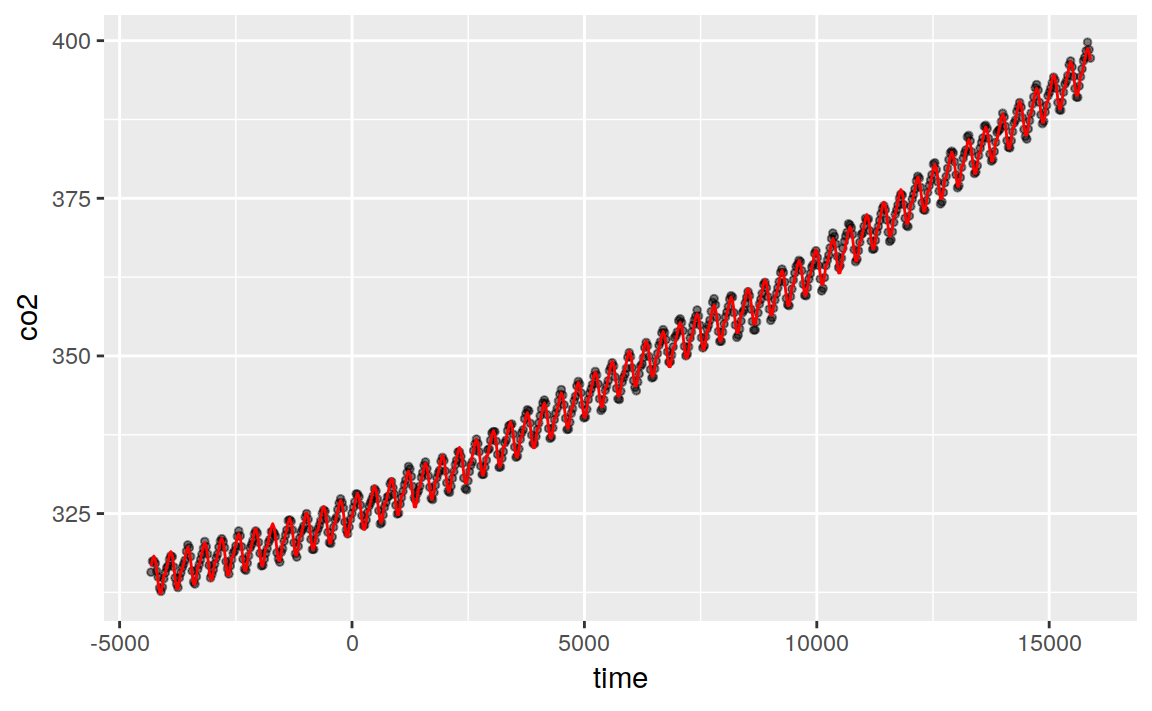
\includegraphics[width=0.7\linewidth]{regression_142-neural_network_yacht_files/figure-latex/unnamed-chunk-13-1} \end{center}

As evident from the plot, we see that the best regression ANN we found was \texttt{Yacht\_NN2} with a training and test SSE of 0.0188 and 0.0057. We make this determination by the value of the training and test SSEs only. \texttt{Yacht\_NN2}'s structure is presented here:

\begin{Shaded}
\begin{Highlighting}[]
\KeywordTok{plot}\NormalTok{(Yacht_NN2, }\DataTypeTok{rep =} \StringTok{"best"}\NormalTok{)}
\end{Highlighting}
\end{Shaded}

\begin{center}\includegraphics[width=0.7\linewidth]{regression_142-neural_network_yacht_files/figure-latex/unnamed-chunk-14-1} \end{center}

\begin{Shaded}
\begin{Highlighting}[]
\KeywordTok{set.seed}\NormalTok{(}\DecValTok{12321}\NormalTok{)}
\NormalTok{Yacht_NN2 <-}\StringTok{ }\KeywordTok{neuralnet}\NormalTok{(Residuary_Resist }\OperatorTok{~}\StringTok{ }\NormalTok{LongPos_COB }\OperatorTok{+}\StringTok{ }\NormalTok{Prismatic_Coeff }\OperatorTok{+}\StringTok{ }\NormalTok{Len_Disp_Ratio }\OperatorTok{+}\StringTok{ }\NormalTok{Beam_Draut_Ratio }\OperatorTok{+}\StringTok{ }\NormalTok{Length_Beam_Ratio }\OperatorTok{+}\StringTok{ }\NormalTok{Froude_Num, }
                       \DataTypeTok{data =}\NormalTok{ Yacht_Data_Train, }
                       \DataTypeTok{hidden =} \KeywordTok{c}\NormalTok{(}\DecValTok{4}\NormalTok{, }\DecValTok{1}\NormalTok{), }
                       \DataTypeTok{act.fct =} \StringTok{"logistic"}\NormalTok{, }
                       \DataTypeTok{rep =} \DecValTok{10}\NormalTok{)}

\KeywordTok{plot}\NormalTok{(Yacht_NN2, }\DataTypeTok{rep =} \StringTok{"best"}\NormalTok{)}
\end{Highlighting}
\end{Shaded}

\begin{center}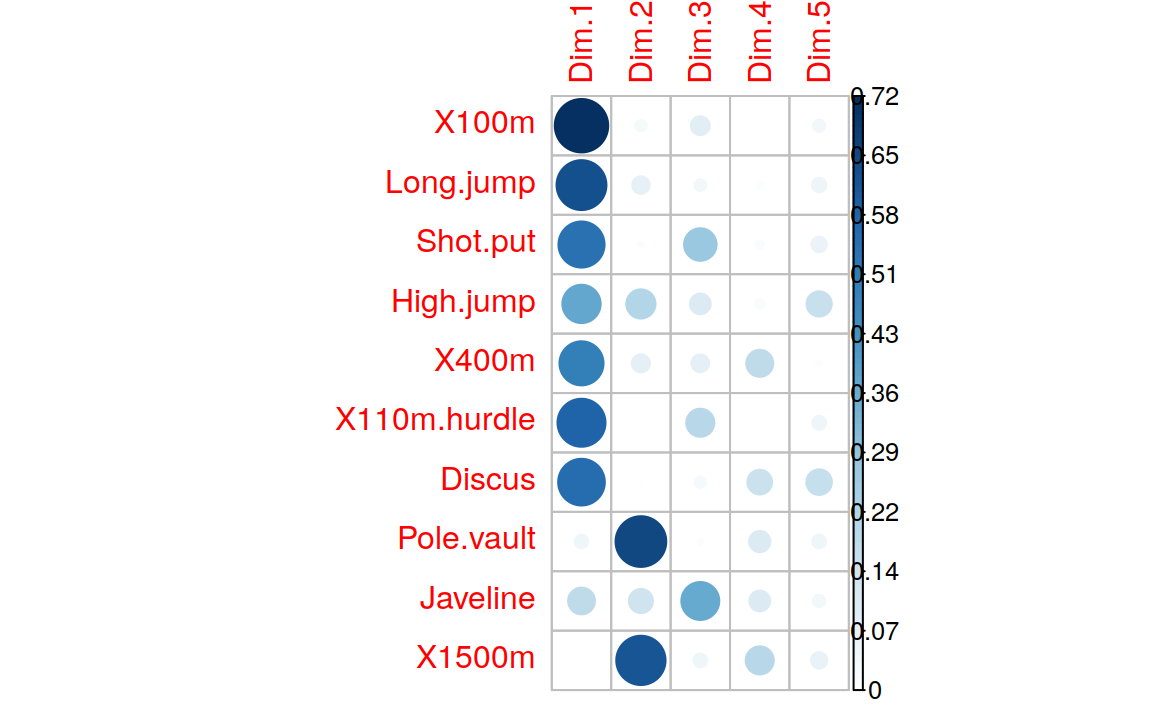
\includegraphics[width=0.7\linewidth]{regression_142-neural_network_yacht_files/figure-latex/unnamed-chunk-15-1} \end{center}

By setting the same seed, prior to running the 10 repetitions of ANNs, we force the software to reproduce the exact same \texttt{Yacht\_NN2} ANN for the first replication. The subsequent 9 generated ANNs, use a different random set of starting weights. Comparing the `best' of the 10 repetitions, to the Yacht\_NN2, we observe a decrease in training set error indicating we have a superior set of weights.

\hypertarget{wrapping-up}{%
\section{Wrapping Up}\label{wrapping-up}}

We have briefly covered regression ANNs in this tutorial. In the next tutorial we will cover classification ANNs. The neuralnet package used in this tutorial is one of many tools available for ANN implementation in R. Others include:

\begin{itemize}
\tightlist
\item
  nnet
\item
  autoencoder
\item
  caret
\item
  RSNNS
\item
  h2o
\end{itemize}

Before you move on to the next tutorial, test your new knowledge on the exercises that follow.

\begin{enumerate}
\def\labelenumi{\arabic{enumi}.}
\item
  Why do we split the yacht data into a training and test data sets?
\item
  Re-load the Yacht Data from the UCI Machine learning repository yacht data without scaling. Run any regression ANN. What happens? Why do you think this happens?
\item
  After completing exercise question 1, re-scale the yacht data. Perform a simple linear regression fitting \texttt{Residuary\_Resist} as a function of all other features. Now run a regression neural network (see 1st Regression ANN section). Plot the regression ANN and compare the weights on the features in the ANN to the p-values for the regressors.
\item
  Build your own regression ANN using the scaled yacht data modifying one hyperparameter. Use \texttt{?neuralnet} to see the function options. Plot your ANN.
\end{enumerate}

\bibliography{book.bib,packages.bib}


\end{document}
